\documentclass[11pt,a4paper]{article}
\usepackage[margin=23mm]{geometry}
\usepackage{fontspec}
\setmainfont{DejaVu Serif}
\setsansfont{DejaVu Sans}
\setmonofont{DejaVu Sans Mono}
\newfontfamily\cjkfont{Droid Sans Fallback}[BoldFont={Droid Sans Fallback}]
\usepackage{graphicx,xcolor,booktabs}
\usepackage[unicode,hidelinks]{hyperref}
\pdfstringdefDisableCommands{\def\cjkfont{}\def\allowbreak{}}
\hypersetup{pdftitle={Turn-table test — 2026-11-03},pdfsubject={Deutsch / English / 简体中文}}
\setlength{\parindent}{0pt}
\setlength{\parskip}{6pt}
\setlength{\emergencystretch}{3em}
\begin{document}
\clearpage\section{Turn-Table-Test — 03.11.2026}

Ausführen (Python 3.10 oder neuer, keine Zusatzpakete):

\begin{quote}\ttfamily\footnotesize python3 turn\_table.py\end{quote}

Anschließend {\small\texttt{ergebnisse/\allowbreak{}index.html}} im Browser öffnen. Alle Diagramme liegen auch einzeln als SVG vor. CSV-Dateien enthalten die Messpositionen, interpolierten Sollpositionen, Fixqualität, Korrekturdatenalter und Ost-/Nord-Abweichungen in Metern. {\small\texttt{auswertung.json}} enthält Fitparameter und Statistik.

Andere Verzeichnisse bzw. maximale Referenzlücke:

\begin{quote}\ttfamily\footnotesize python3 turn\_table.py --input-dir . --output-dir ergebnisse --max-gap 3\end{quote}

\subsection{Verfahren und zeitliche Zuordnung}

NMEA-Prüfsummen werden geprüft, ungültige Positionen (Qualität 0) verworfen. Auch wörtlich gespeicherte {\small\texttt{\textbackslash{}r\textbackslash{}n}} werden unterstützt. Zeitbasis sind die UTC-Epochen der GGA-Sätze, nicht Dateibeginn oder Zeilennummer. Tageswechsel werden erkannt. Das Datum 03.11.2026 kommt aus UM980-RMC; mangels Datumsinformation in den beiden P23A-Dateien wird für sie derselbe Tag angenommen. Eine unbekannte interne Messlatenz lässt sich allein aus GGA nicht unabhängig prüfen; es wird keine nachträgliche Zeitverschiebung geschätzt.

WGS84-Breite/Länge werden mit den lokalen WGS84-Krümmungsradien in Ost-/Nord-Meter umgerechnet (für diesen kleinen Messbereich ausreichend). Ein geometrischer Kreisfit mit Huber-Gewichten bestimmt Mittelpunkt und Radius aus den RTK-fixed-Positionen (GGA-Qualität 4) von P23A\_0. Der Kreisfit verwendet die ganze verfügbare Fixed-Referenz.

Der Referenzwinkel ist {\small\texttt{atan2(Nord-Mittelpunkt\_\allowbreak{}Nord, Ost-Mittelpunkt\_\allowbreak{}Ost)}}, positiv von Ost nach Nord. Die Winkelgrafik zeigt den relativen Drehwinkel geteilt durch 360° als Anzahl der Vollkreise seit dem ersten Referenzpunkt (einschließlich Bruchteilen). Die CSV-Dateien enthalten zusätzlich diese Umdrehungszahl. Seine zeitliche Entwicklung wird entfaltet; es wird keine konstante Drehgeschwindigkeit vorausgesetzt. Radiale Referenzausreißer oberhalb von max(2 cm, 6 robusten Standardabweichungen) werden für die Winkelbestimmung ausgeschlossen. Bei diesen Daten wurden keine Fixed-Punkte dadurch ausgeschlossen.

Ausgewertet wird der gemeinsame Zeitraum mit verfügbarer Fixed-Referenz. Der entfaltete Winkel wird bei Bedarf zwischen benachbarten zuverlässigen Referenzepochen interpoliert, höchstens über {\small\texttt{--max-gap}} Sekunden. Keine Extrapolation. Vor dem RTK-fixed-Filter stimmen die 13.191 zeitlich zuordenbaren Epochen aller drei Receiver exakt überein; eine Interpolation ist daher hier nicht nötig. Nach dem Filter enthält jeder Receiver nur seine eigenen RTK-fixed-Epochen; die Zeitzuordnung zur Referenz bleibt unverändert. Zwei größere Referenzlücken werden ausgespart. Über solche Lücken ist die Zahl ganzer Umdrehungen unbekannt; der Winkel wird anschließend mit dem nächstliegenden Winkel fortgesetzt. Die Segmentnummer steht in {\small\texttt{referenz\_\allowbreak{}winkel.csv}}.

Für jede verwendete Messung gilt:

\begin{quote}\ttfamily\footnotesize Soll\_Ost  = Mittelpunkt\_Ost  + R*cos(Winkel(t))\\Soll\_Nord = Mittelpunkt\_Nord + R*sin(Winkel(t))\\Fehler    = Messposition(t) - Sollposition(t)\end{quote}

Nur RTK-fixed-Positionen (GGA-Qualität 4) werden in Ergebnis-CSV, Diagrammen und Fehlerstatistiken berücksichtigt. GGA-Qualität 4 allein beweist keinen aktiven Empfang von Referenzdaten. Die Outage-Schaltzeiten werden daher nicht aus der Fixqualität oder dem ungefähren 3-/5-Minuten-Zyklus erfunden. Das gemeldete Korrekturdatenalter ist in den CSV-Dateien enthalten.

Da der Sollwinkel aus P23A\_0 selbst stammt, kann dessen tangentialer Fehler nicht unabhängig bestimmt werden. Die rote Spur zeigt hauptsächlich den radialen Restfehler. Gemeinsame systematische Fehler aller Receiver können mit dieser Referenzannahme ebenfalls nicht aufgedeckt werden.

\subsection{Ergebnis}

Mittlere Umdrehungsdauer: \textbf{169,599 s} (\ensuremath{\approx} \textbf{2 min 49,6 s}), arithmetisches Mittel aus \textbf{76 vollständigen Umdrehungen}. Standardabweichung: \textbf{15,028 s}, Minimum: \textbf{160,797 s}, Maximum: \textbf{292,545 s}.

Je zusammenhängendem Referenzsegment werden ausgehend vom ersten verwendeten Winkel die Zeitpunkte aufeinanderfolgender 360°-Fortschritte bestimmt; die Durchgangszeiten werden zwischen benachbarten Epochen linear interpoliert. Die Dauer jeder vollständigen Umdrehung geht gleich gewichtet in den Mittelwert ein. Unvollständige Umdrehungen am Segmentende und Referenzlücken werden ausgeschlossen. Langsamere Abschnitte oder Stillstände innerhalb einer vollständigen Umdrehung bleiben enthalten. Einzelwerte und Segmentnummern stehen in {\small\texttt{ergebnisse/\allowbreak{}umdrehungsdauer.csv}}, Kennwerte zusätzlich in {\small\texttt{auswertung.json}}.

Radius: \textbf{0,330966 m}. Gemeinsamer auswertbarer Zeitraum: \textbf{03:41:09–08:15:08 UTC}, mit ausgesparten Referenzlücken.

\begin{center}\small\begin{tabular}{lrrr}\toprule
Receiver & RMS horizontal & 95\%-Quantil & Maximum\\\midrule
P23A\_0 & 0,00383 m & 0,00769 m & 0,01710 m\\
P23A\_1 & 0,01746 m & 0,03542 m & 0,09647 m\\
UM980 & 0,02071 m & 0,04256 m & 0,07939 m\\
\bottomrule\end{tabular}\end{center}

Die vollständige horizontale Ansicht enthält sämtliche RTK-fixed-Abweichungen; die zusätzliche Detailansicht zeigt ±10 cm und blendet Punkte außerhalb aus. Gleiche Achsenskalierung, rot=P23A\_0, grün=P23A\_1, blau=UM980, schwarzes Kreuz=Sollposition. Zusätzlich: Anzahl der Vollkreise, Ost-, Nord- und horizontaler Fehler über der Zeit. Statistiken beziehen sich auf alle verwendeten Epochen, nicht nur auf das Detailfenster oder einzelne Outage-Phasen.

Validiert durch vollständigen Lauf mit den drei Eingabedateien, identische Ergebnis-Zeitstempel, einen synthetischen Kreis mit bekanntem Mittelpunkt/Radius und einen GGA-Mitternachtswechsel.

\subsection{Fazit zum Outage-Vergleich}

\textbf{P23A\_1 zeigt die kleineren typischen horizontalen Abweichungen während Abschnitten mit veralteten Referenzdaten.} Der UM980 hat dagegen den kleineren maximalen Einzelfehler. P23A\_0 dient als kontinuierlich versorgte Referenz und wird nicht als Outage-Kandidat gewertet.

Für einen fairen direkten Vergleich werden 6.812 identische UTC-Epochen ausgewählt: beide Receiver RTK-fixed, beide mit gemeldetem Korrekturdatenalter >10 s. Das ist ein nachvollziehbarer Indikator für veraltete Korrekturen, kein externes Protokoll der tatsächlichen Schaltzeiten. Nicht-fixed-Positionen und Referenzlücken sind ausgeschlossen. Das Fazit bewertet die Genauigkeit der verbleibenden Fixed-Lösungen, nicht die vollständige Verfügbarkeit über sämtliche Outage-Phasen.

\begin{center}\small\begin{tabular}{lrrrr}\toprule
Receiver & RMS & Median & 95\%-Quantil & Maximum\\\midrule
P23A\_1 & 1,89 cm & 1,30 cm & 3,59 cm & 9,65 cm\\
UM980 & 2,69 cm & 1,90 cm & 5,42 cm & 7,94 cm\\
\bottomrule\end{tabular}\end{center}

Damit liegt der RMS von P23A\_1 in diesem Vergleich rund 30 \% unter dem des UM980. Die einzelnen Vergleichsepochen stehen in {\small\texttt{ergebnisse/\allowbreak{}outage\_\allowbreak{}vergleich.csv}}, die Statistik in {\small\texttt{auswertung.json}}.

\begin{figure}[p]\centering
\resizebox{0.98\linewidth}{!}{%
\setlength{\unitlength}{1bp}\begin{picture}(680.0,680.0)
\put(0,0){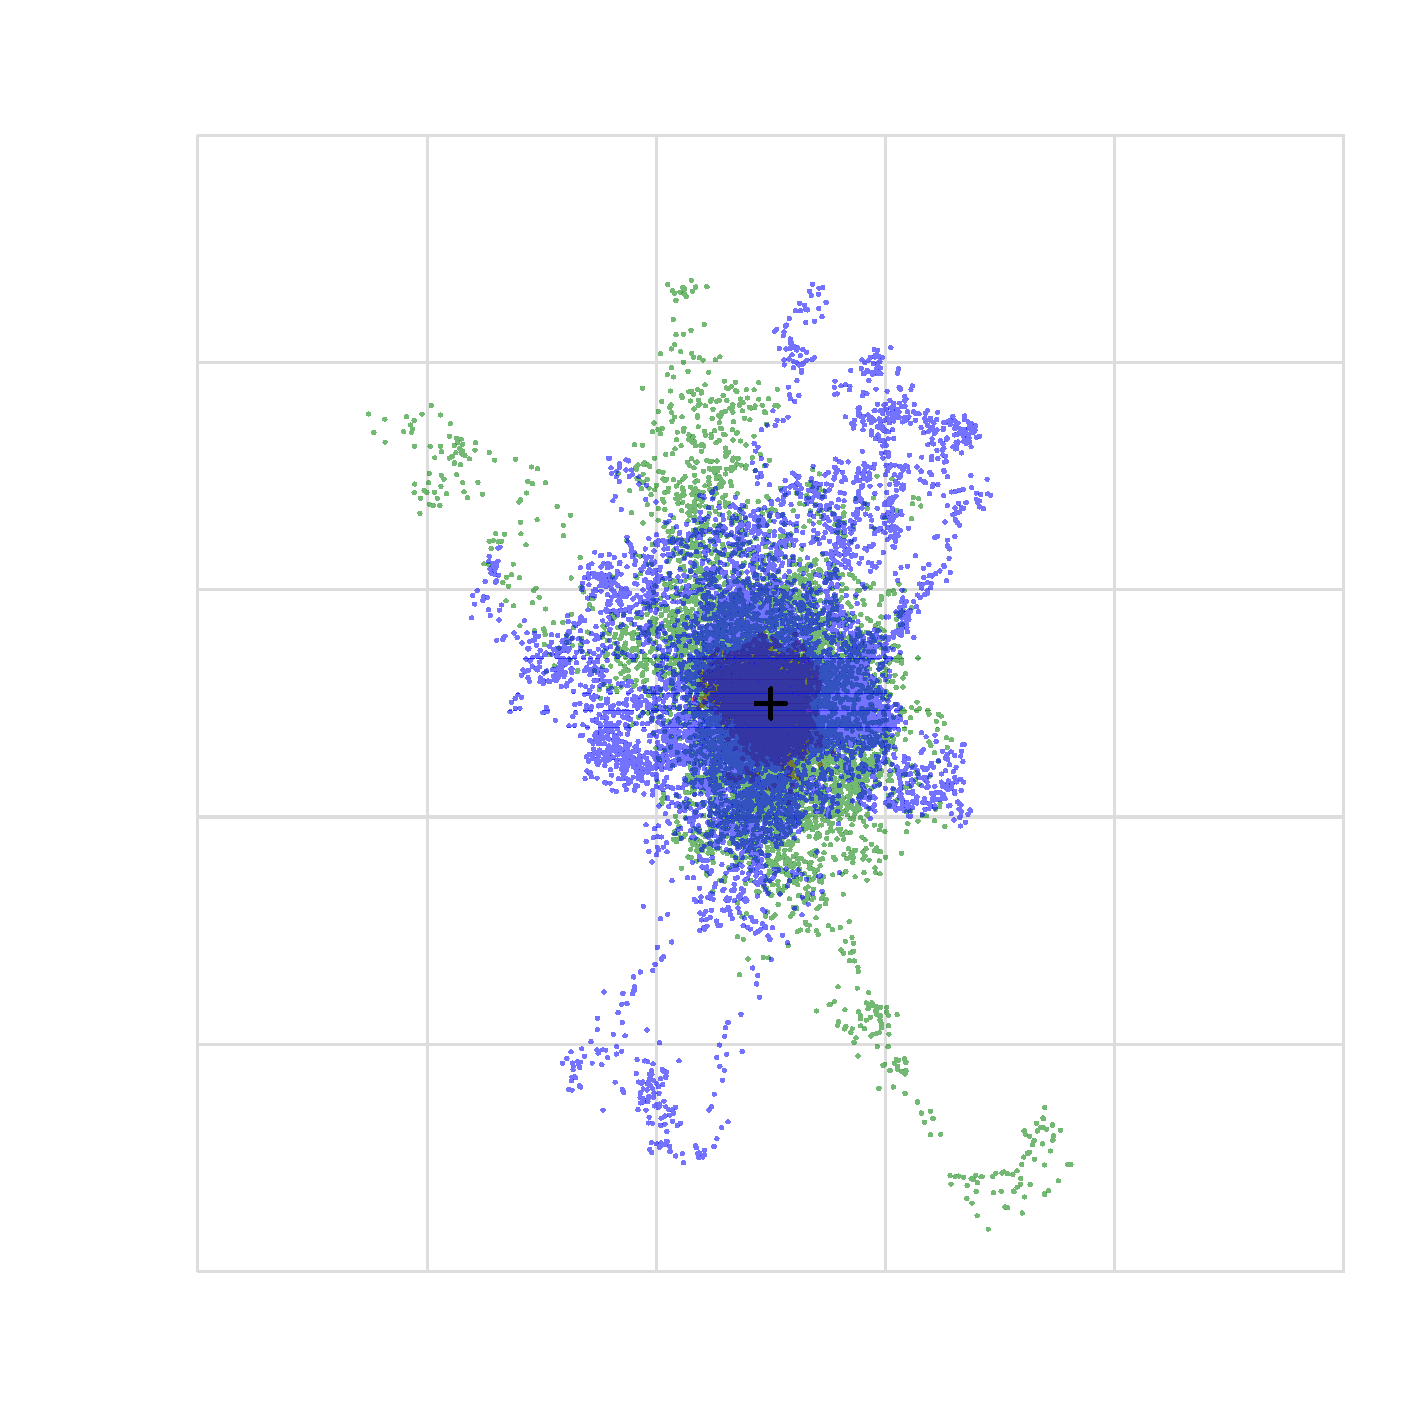
\includegraphics[width=680.0bp,height=680.0bp]{bericht/abbildungen/horizontal.pdf}}
\put(95.0,657.0){\makebox(0,0)[lb]{\color{black}\sffamily\fontsize{16}{16}\selectfont Horizontale Abweichungen vom zeitgleichen Sollkreis}}
\put(95.0,50.0){\makebox(0,0)[cb]{\color{black}\sffamily\fontsize{12}{12}\selectfont -0.09642}}
\put(87.0,66.0){\makebox(0,0)[rb]{\color{black}\sffamily\fontsize{12}{12}\selectfont -0.09642}}
\put(205.0,50.0){\makebox(0,0)[cb]{\color{black}\sffamily\fontsize{12}{12}\selectfont -0.05785}}
\put(87.0,175.0){\makebox(0,0)[rb]{\color{black}\sffamily\fontsize{12}{12}\selectfont -0.05785}}
\put(315.0,50.0){\makebox(0,0)[cb]{\color{black}\sffamily\fontsize{12}{12}\selectfont -0.01928}}
\put(87.0,284.0){\makebox(0,0)[rb]{\color{black}\sffamily\fontsize{12}{12}\selectfont -0.01928}}
\put(425.00000000000006,50.0){\makebox(0,0)[cb]{\color{black}\sffamily\fontsize{12}{12}\selectfont 0.01928}}
\put(87.0,393.00000000000006){\makebox(0,0)[rb]{\color{black}\sffamily\fontsize{12}{12}\selectfont 0.01928}}
\put(535.0,50.0){\makebox(0,0)[cb]{\color{black}\sffamily\fontsize{12}{12}\selectfont 0.05785}}
\put(87.0,501.99999999999994){\makebox(0,0)[rb]{\color{black}\sffamily\fontsize{12}{12}\selectfont 0.05785}}
\put(645.0,50.0){\makebox(0,0)[cb]{\color{black}\sffamily\fontsize{12}{12}\selectfont 0.09642}}
\put(87.0,611.0){\makebox(0,0)[rb]{\color{black}\sffamily\fontsize{12}{12}\selectfont 0.09642}}
\put(95.0,635.0){\makebox(0,0)[lb]{\color{red}\sffamily\fontsize{12}{12}\selectfont P23A\_0}}
\put(265.0,635.0){\makebox(0,0)[lb]{\color{green}\sffamily\fontsize{12}{12}\selectfont P23A\_1}}
\put(435.0,635.0){\makebox(0,0)[lb]{\color{blue}\sffamily\fontsize{12}{12}\selectfont UM980}}
\put(379.0,351.5){\makebox(0,0)[lb]{\color{black}\sffamily\fontsize{12}{12}\selectfont Soll (0,0)}}
\put(370.0,12.0){\makebox(0,0)[cb]{\color{black}\sffamily\fontsize{12}{12}\selectfont Ost-Abweichung [m]}}
\put(19.0,342.5){\rotatebox{90}{\makebox(0,0)[b]{\color{black}\sffamily\fontsize{12}{12}\selectfont Nord-Abweichung [m]}}}
\end{picture}}
\end{figure}
\begin{figure}[p]\centering
\resizebox{0.98\linewidth}{!}{%
\setlength{\unitlength}{1bp}\begin{picture}(680.0,680.0)
\put(0,0){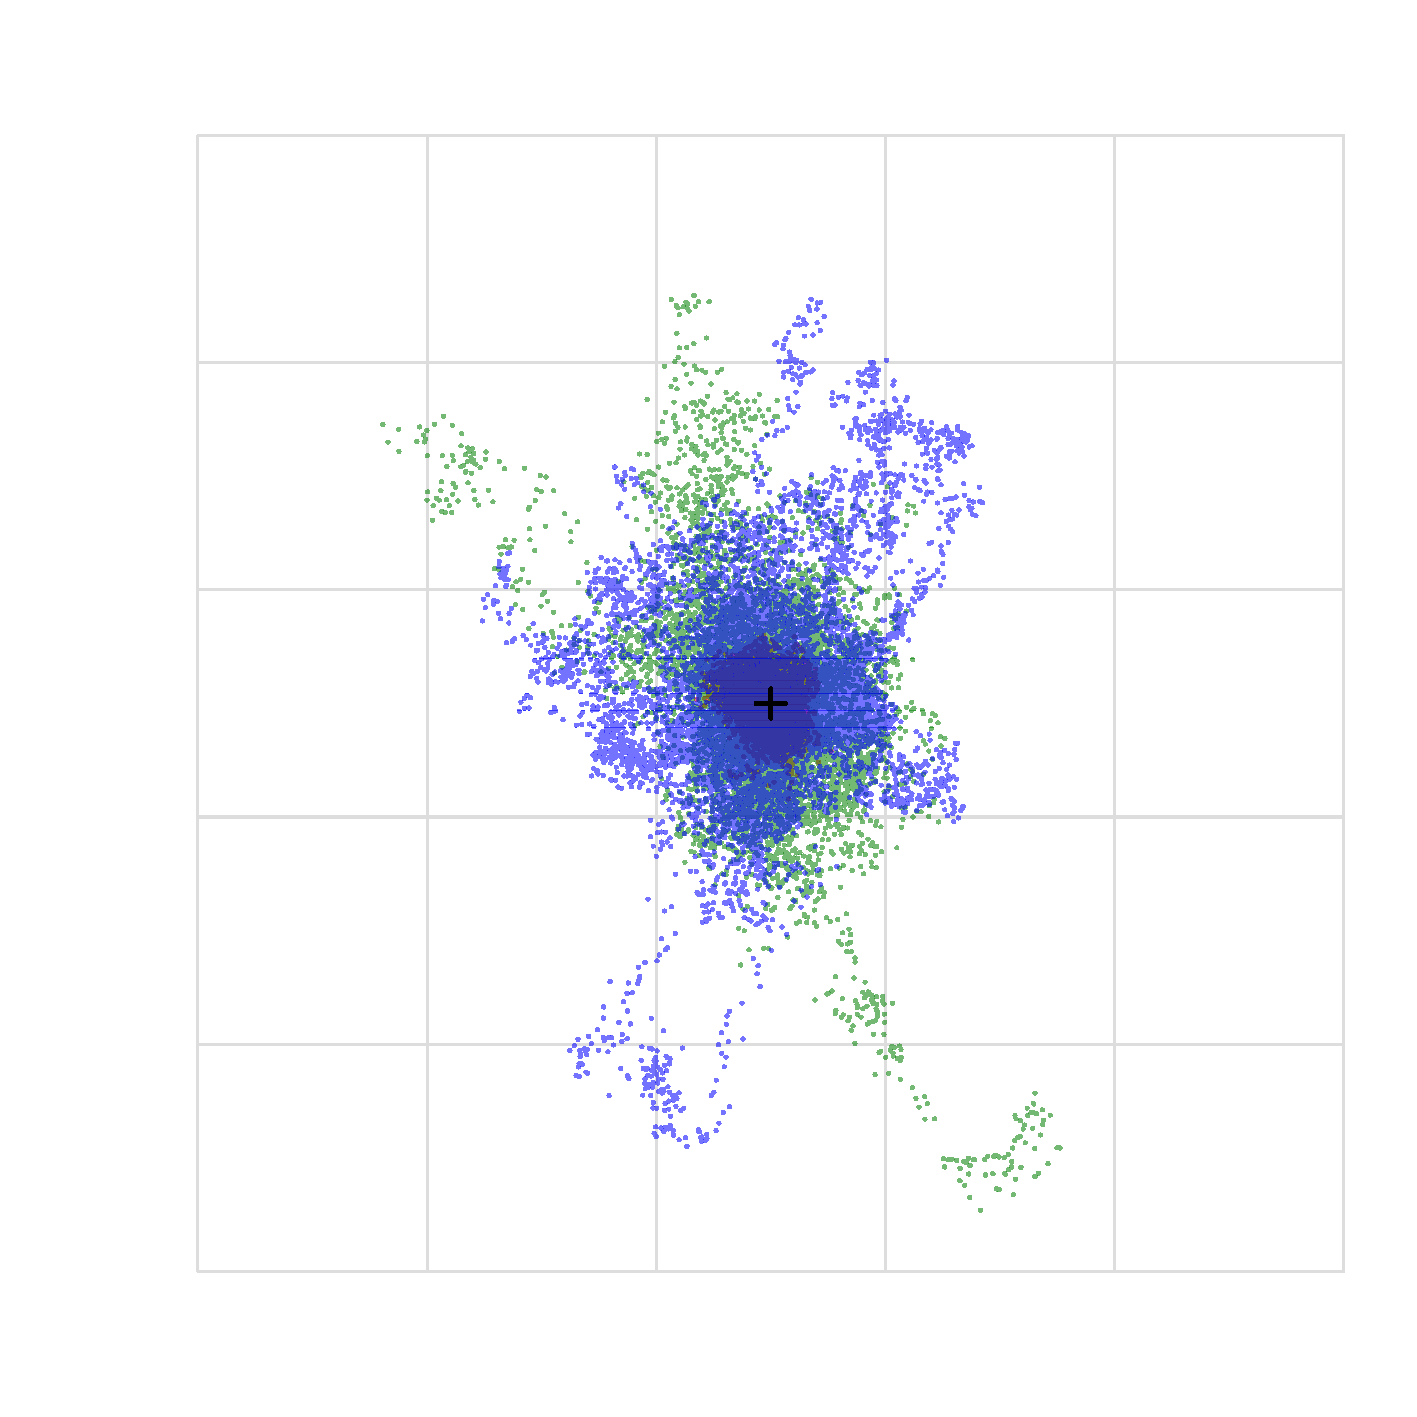
\includegraphics[width=680.0bp,height=680.0bp]{bericht/abbildungen/horizontal_detail.pdf}}
\put(95.0,657.0){\makebox(0,0)[lb]{\color{black}\sffamily\fontsize{16}{16}\selectfont Detail ±0,10 m (größere Abweichungen ausgeblendet)}}
\put(95.0,50.0){\makebox(0,0)[cb]{\color{black}\sffamily\fontsize{12}{12}\selectfont -0.1}}
\put(87.0,66.0){\makebox(0,0)[rb]{\color{black}\sffamily\fontsize{12}{12}\selectfont -0.1}}
\put(205.0,50.0){\makebox(0,0)[cb]{\color{black}\sffamily\fontsize{12}{12}\selectfont -0.06}}
\put(87.0,175.0){\makebox(0,0)[rb]{\color{black}\sffamily\fontsize{12}{12}\selectfont -0.06}}
\put(315.0,50.0){\makebox(0,0)[cb]{\color{black}\sffamily\fontsize{12}{12}\selectfont -0.02}}
\put(87.0,284.0){\makebox(0,0)[rb]{\color{black}\sffamily\fontsize{12}{12}\selectfont -0.02}}
\put(425.00000000000006,50.0){\makebox(0,0)[cb]{\color{black}\sffamily\fontsize{12}{12}\selectfont 0.02}}
\put(87.0,393.00000000000006){\makebox(0,0)[rb]{\color{black}\sffamily\fontsize{12}{12}\selectfont 0.02}}
\put(535.0,50.0){\makebox(0,0)[cb]{\color{black}\sffamily\fontsize{12}{12}\selectfont 0.06}}
\put(87.0,501.99999999999994){\makebox(0,0)[rb]{\color{black}\sffamily\fontsize{12}{12}\selectfont 0.06}}
\put(645.0,50.0){\makebox(0,0)[cb]{\color{black}\sffamily\fontsize{12}{12}\selectfont 0.1}}
\put(87.0,611.0){\makebox(0,0)[rb]{\color{black}\sffamily\fontsize{12}{12}\selectfont 0.1}}
\put(95.0,635.0){\makebox(0,0)[lb]{\color{red}\sffamily\fontsize{12}{12}\selectfont P23A\_0}}
\put(265.0,635.0){\makebox(0,0)[lb]{\color{green}\sffamily\fontsize{12}{12}\selectfont P23A\_1}}
\put(435.0,635.0){\makebox(0,0)[lb]{\color{blue}\sffamily\fontsize{12}{12}\selectfont UM980}}
\put(379.0,351.5){\makebox(0,0)[lb]{\color{black}\sffamily\fontsize{12}{12}\selectfont Soll (0,0)}}
\put(370.0,12.0){\makebox(0,0)[cb]{\color{black}\sffamily\fontsize{12}{12}\selectfont Ost-Abweichung [m]}}
\put(19.0,342.5){\rotatebox{90}{\makebox(0,0)[b]{\color{black}\sffamily\fontsize{12}{12}\selectfont Nord-Abweichung [m]}}}
\end{picture}}
\end{figure}
\begin{figure}[p]\centering
\resizebox{0.98\linewidth}{!}{%
\setlength{\unitlength}{1bp}\begin{picture}(1000.0,430.0)
\put(0,0){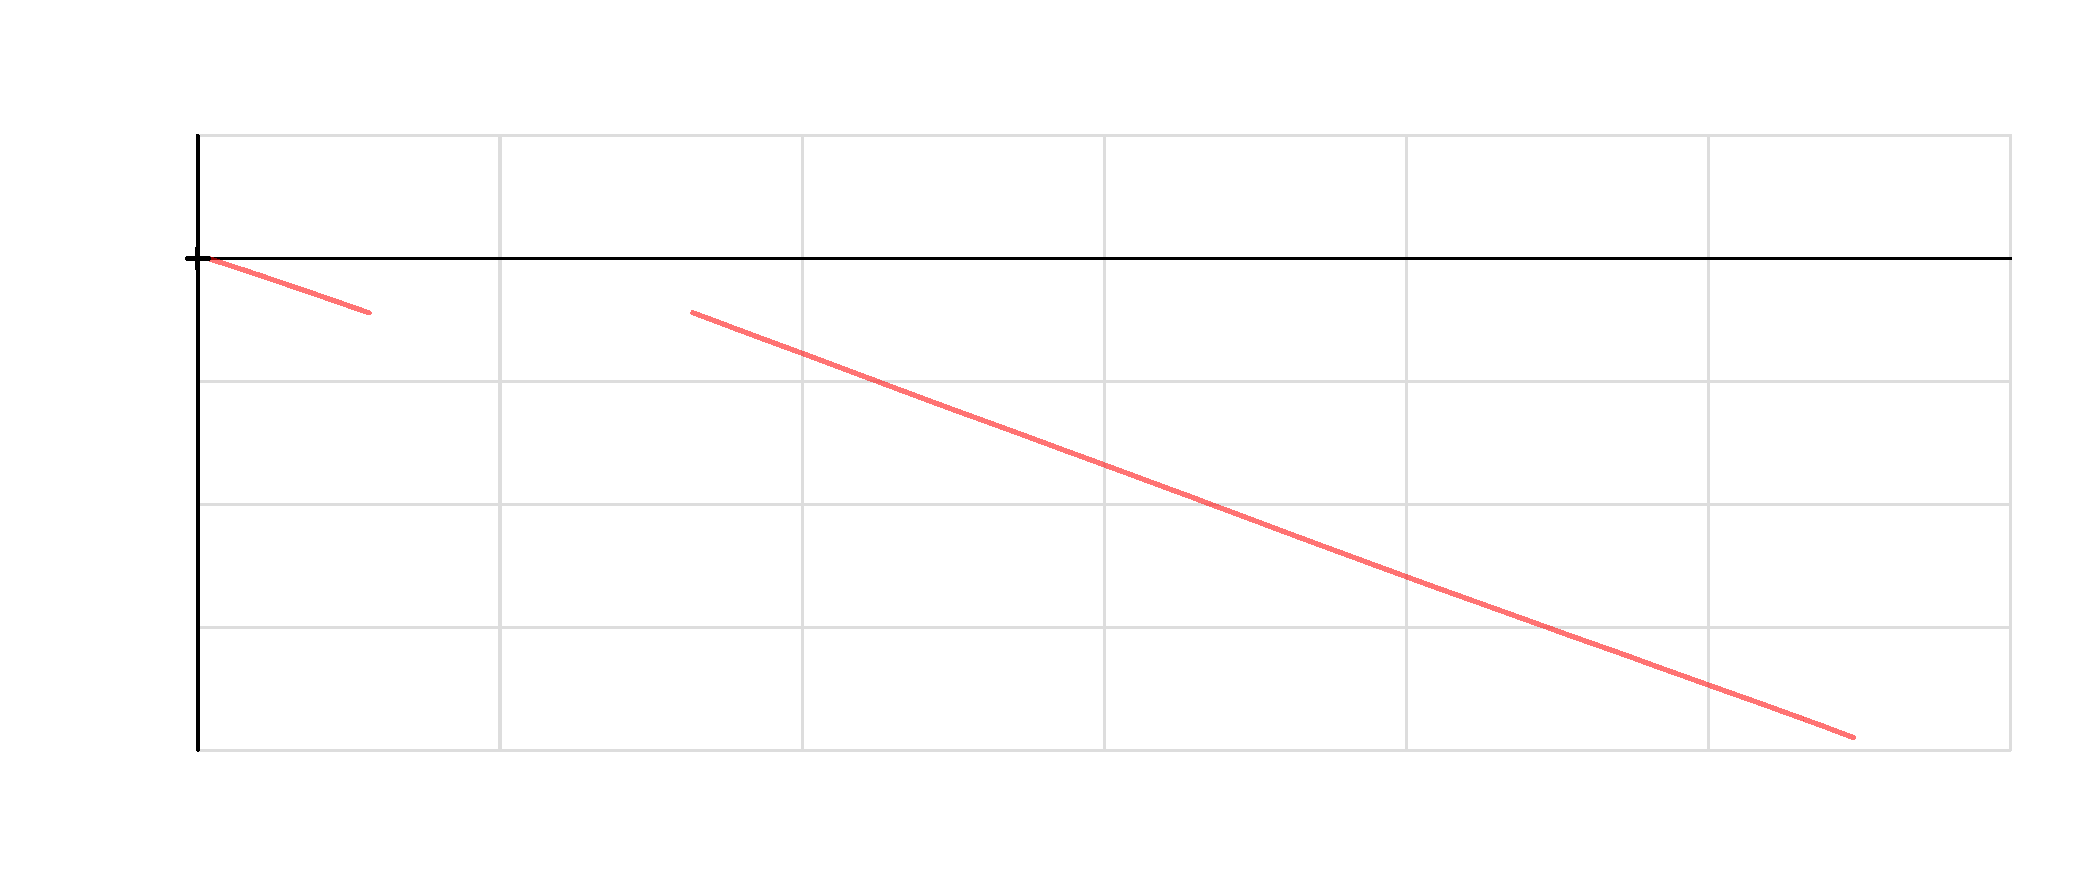
\includegraphics[width=1000.0bp,height=430.0bp]{bericht/abbildungen/winkel.pdf}}
\put(95.0,407.0){\makebox(0,0)[lb]{\color{black}\sffamily\fontsize{16}{16}\selectfont Umdrehungen: positiv von Ost nach Nord}}
\put(95.0,50.0){\makebox(0,0)[cb]{\color{black}\sffamily\fontsize{12}{12}\selectfont -10.96}}
\put(87.0,66.0){\makebox(0,0)[rb]{\color{black}\sffamily\fontsize{12}{12}\selectfont -84.19}}
\put(269.0,50.0){\makebox(0,0)[cb]{\color{black}\sffamily\fontsize{12}{12}\selectfont 48.22}}
\put(87.0,125.0){\makebox(0,0)[rb]{\color{black}\sffamily\fontsize{12}{12}\selectfont -66.1}}
\put(442.99999999999994,50.0){\makebox(0,0)[cb]{\color{black}\sffamily\fontsize{12}{12}\selectfont 107.4}}
\put(87.0,184.0){\makebox(0,0)[rb]{\color{black}\sffamily\fontsize{12}{12}\selectfont -48.02}}
\put(617.0000000000001,50.0){\makebox(0,0)[cb]{\color{black}\sffamily\fontsize{12}{12}\selectfont 166.6}}
\put(87.0,243.00000000000003){\makebox(0,0)[rb]{\color{black}\sffamily\fontsize{12}{12}\selectfont -29.93}}
\put(790.9999999999999,50.0){\makebox(0,0)[cb]{\color{black}\sffamily\fontsize{12}{12}\selectfont 225.8}}
\put(87.0,302.0){\makebox(0,0)[rb]{\color{black}\sffamily\fontsize{12}{12}\selectfont -11.85}}
\put(965.0,50.0){\makebox(0,0)[cb]{\color{black}\sffamily\fontsize{12}{12}\selectfont 284.9}}
\put(87.0,361.0){\makebox(0,0)[rb]{\color{black}\sffamily\fontsize{12}{12}\selectfont 6.24}}
\put(95.0,385.0){\makebox(0,0)[lb]{\color{red}\sffamily\fontsize{12}{12}\selectfont P23A\_0}}
\put(530.0,12.0){\makebox(0,0)[cb]{\color{black}\sffamily\fontsize{12}{12}\selectfont Zeit seit gemeinsamem Beginn [min]}}
\put(19.0,217.5){\rotatebox{90}{\makebox(0,0)[b]{\color{black}\sffamily\fontsize{12}{12}\selectfont Anzahl der Vollkreise seit erstem Referenzpunkt}}}
\end{picture}}
\end{figure}
\begin{figure}[p]\centering
\resizebox{0.98\linewidth}{!}{%
\setlength{\unitlength}{1bp}\begin{picture}(1000.0,430.0)
\put(0,0){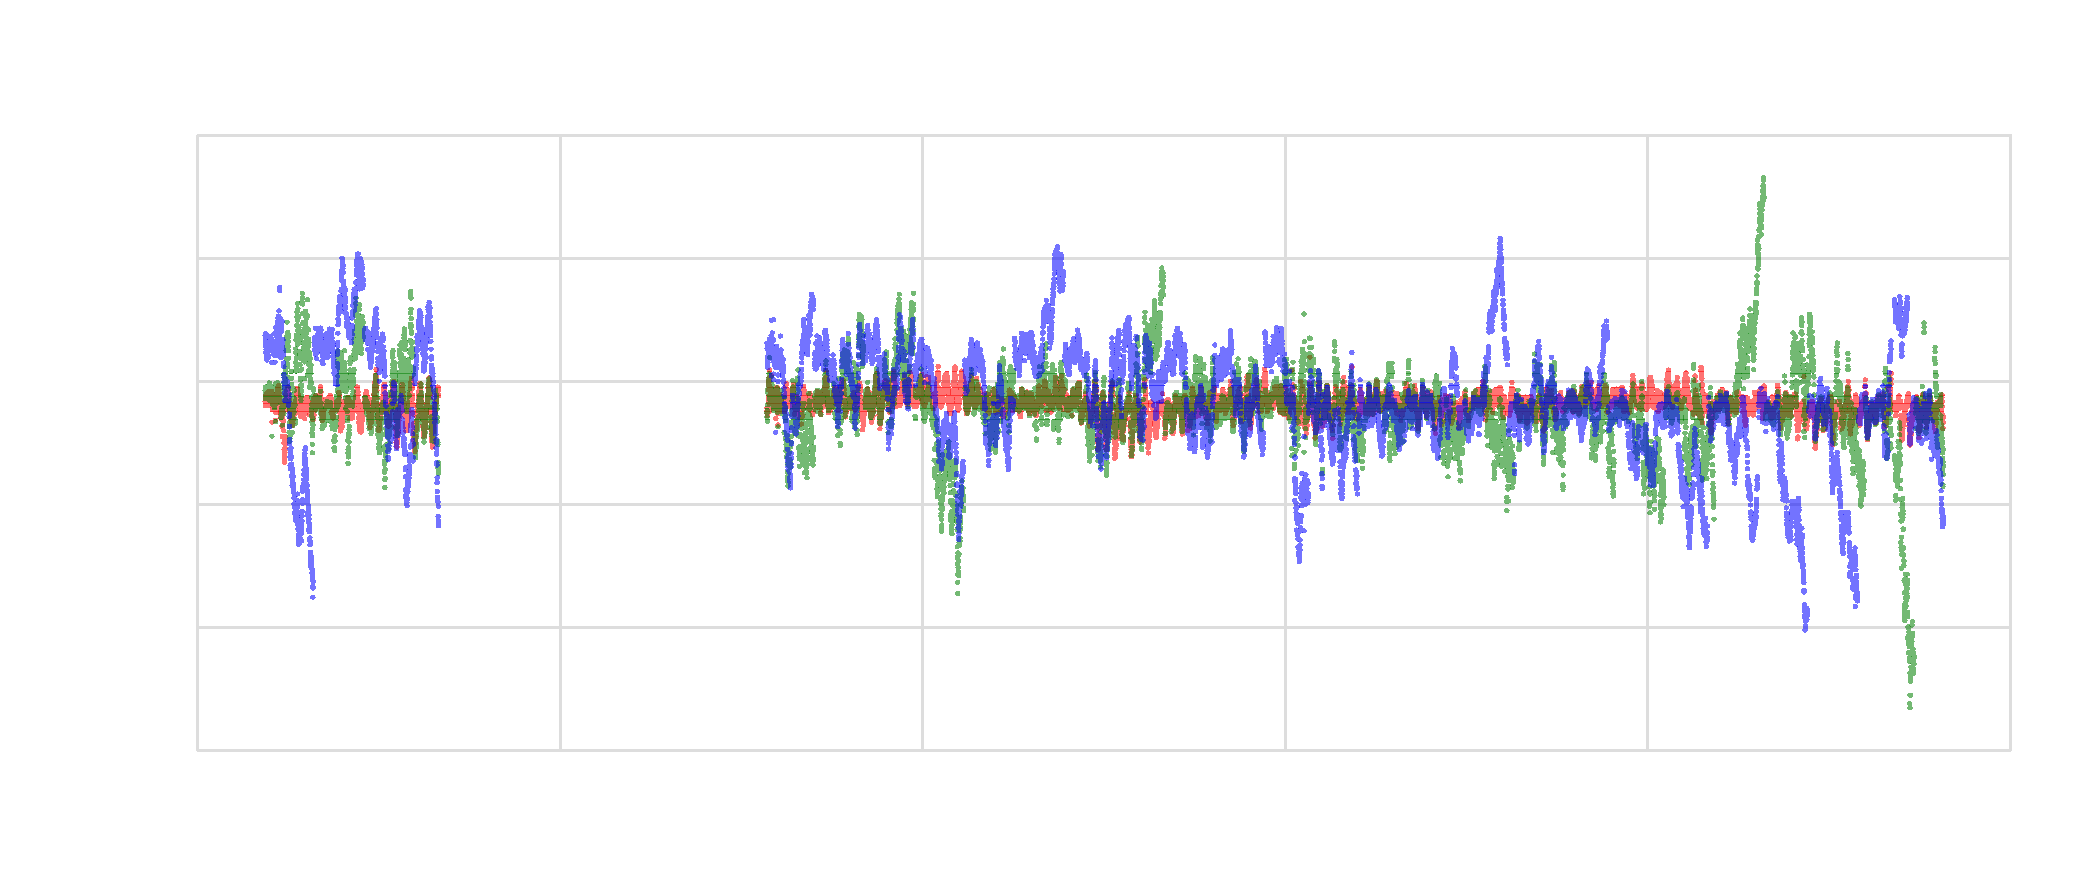
\includegraphics[width=1000.0bp,height=430.0bp]{bericht/abbildungen/east_zeit.pdf}}
\put(95.0,407.0){\makebox(0,0)[lb]{\color{black}\sffamily\fontsize{16}{16}\selectfont Ost-Abweichung über der Zeit}}
\put(95.0,50.0){\makebox(0,0)[cb]{\color{black}\sffamily\fontsize{12}{12}\selectfont -10.96}}
\put(87.0,66.0){\makebox(0,0)[rb]{\color{black}\sffamily\fontsize{12}{12}\selectfont -0.0772}}
\put(269.0,50.0){\makebox(0,0)[cb]{\color{black}\sffamily\fontsize{12}{12}\selectfont 48.22}}
\put(87.0,125.0){\makebox(0,0)[rb]{\color{black}\sffamily\fontsize{12}{12}\selectfont -0.04977}}
\put(442.99999999999994,50.0){\makebox(0,0)[cb]{\color{black}\sffamily\fontsize{12}{12}\selectfont 107.4}}
\put(87.0,184.0){\makebox(0,0)[rb]{\color{black}\sffamily\fontsize{12}{12}\selectfont -0.02235}}
\put(617.0000000000001,50.0){\makebox(0,0)[cb]{\color{black}\sffamily\fontsize{12}{12}\selectfont 166.6}}
\put(87.0,243.0){\makebox(0,0)[rb]{\color{black}\sffamily\fontsize{12}{12}\selectfont 0.005077}}
\put(790.9999999999999,50.0){\makebox(0,0)[cb]{\color{black}\sffamily\fontsize{12}{12}\selectfont 225.8}}
\put(87.0,302.0){\makebox(0,0)[rb]{\color{black}\sffamily\fontsize{12}{12}\selectfont 0.0325}}
\put(965.0,50.0){\makebox(0,0)[cb]{\color{black}\sffamily\fontsize{12}{12}\selectfont 284.9}}
\put(87.0,361.0){\makebox(0,0)[rb]{\color{black}\sffamily\fontsize{12}{12}\selectfont 0.05993}}
\put(95.0,385.0){\makebox(0,0)[lb]{\color{red}\sffamily\fontsize{12}{12}\selectfont P23A\_0}}
\put(265.0,385.0){\makebox(0,0)[lb]{\color{green}\sffamily\fontsize{12}{12}\selectfont P23A\_1}}
\put(435.0,385.0){\makebox(0,0)[lb]{\color{blue}\sffamily\fontsize{12}{12}\selectfont UM980}}
\put(530.0,12.0){\makebox(0,0)[cb]{\color{black}\sffamily\fontsize{12}{12}\selectfont Zeit seit gemeinsamem Beginn [min]}}
\put(19.0,217.5){\rotatebox{90}{\makebox(0,0)[b]{\color{black}\sffamily\fontsize{12}{12}\selectfont Ost-Abweichung [m]}}}
\end{picture}}
\end{figure}
\begin{figure}[p]\centering
\resizebox{0.98\linewidth}{!}{%
\setlength{\unitlength}{1bp}\begin{picture}(1000.0,430.0)
\put(0,0){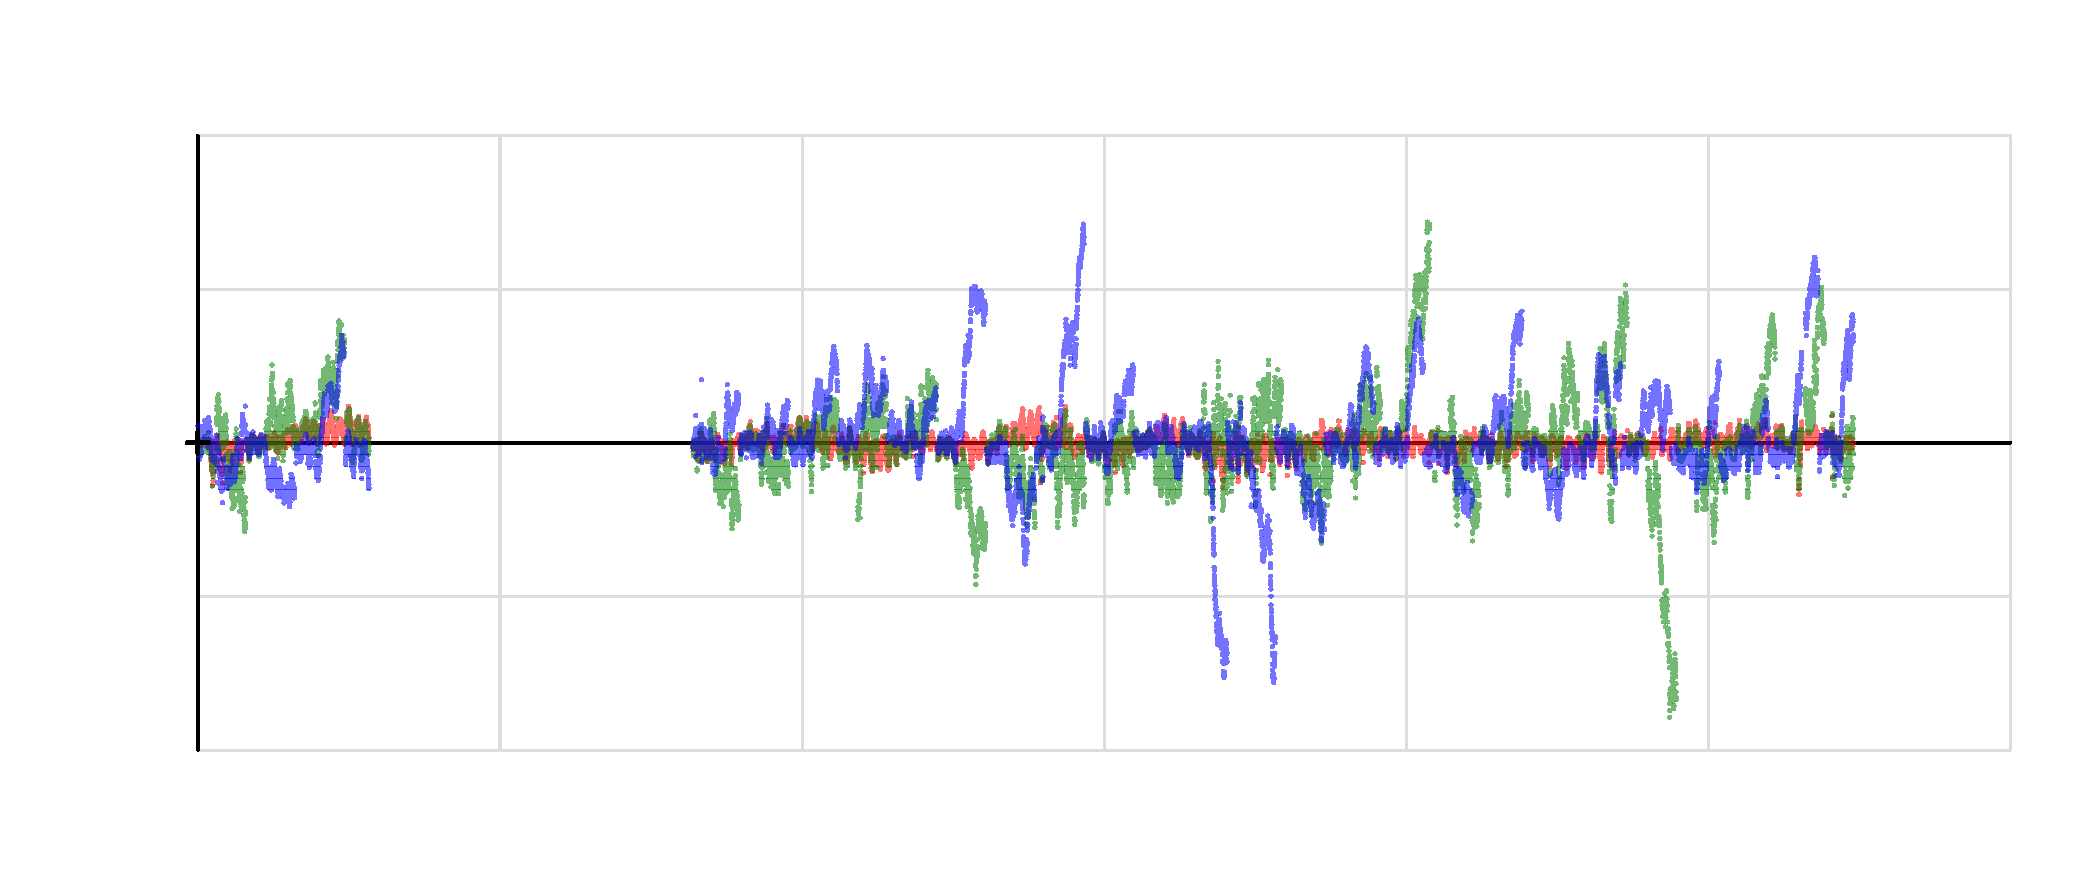
\includegraphics[width=1000.0bp,height=430.0bp]{bericht/abbildungen/north_zeit.pdf}}
\put(95.0,407.0){\makebox(0,0)[lb]{\color{black}\sffamily\fontsize{16}{16}\selectfont Nord-Abweichung über der Zeit}}
\put(95.0,50.0){\makebox(0,0)[cb]{\color{black}\sffamily\fontsize{12}{12}\selectfont -10.96}}
\put(87.0,66.0){\makebox(0,0)[rb]{\color{black}\sffamily\fontsize{12}{12}\selectfont -0.1022}}
\put(269.0,50.0){\makebox(0,0)[cb]{\color{black}\sffamily\fontsize{12}{12}\selectfont 48.22}}
\put(87.0,125.0){\makebox(0,0)[rb]{\color{black}\sffamily\fontsize{12}{12}\selectfont -0.06478}}
\put(442.99999999999994,50.0){\makebox(0,0)[cb]{\color{black}\sffamily\fontsize{12}{12}\selectfont 107.4}}
\put(87.0,184.0){\makebox(0,0)[rb]{\color{black}\sffamily\fontsize{12}{12}\selectfont -0.0274}}
\put(617.0000000000001,50.0){\makebox(0,0)[cb]{\color{black}\sffamily\fontsize{12}{12}\selectfont 166.6}}
\put(87.0,243.0){\makebox(0,0)[rb]{\color{black}\sffamily\fontsize{12}{12}\selectfont 0.00999}}
\put(790.9999999999999,50.0){\makebox(0,0)[cb]{\color{black}\sffamily\fontsize{12}{12}\selectfont 225.8}}
\put(87.0,302.0){\makebox(0,0)[rb]{\color{black}\sffamily\fontsize{12}{12}\selectfont 0.04738}}
\put(965.0,50.0){\makebox(0,0)[cb]{\color{black}\sffamily\fontsize{12}{12}\selectfont 284.9}}
\put(87.0,361.0){\makebox(0,0)[rb]{\color{black}\sffamily\fontsize{12}{12}\selectfont 0.08476}}
\put(95.0,385.0){\makebox(0,0)[lb]{\color{red}\sffamily\fontsize{12}{12}\selectfont P23A\_0}}
\put(265.0,385.0){\makebox(0,0)[lb]{\color{green}\sffamily\fontsize{12}{12}\selectfont P23A\_1}}
\put(435.0,385.0){\makebox(0,0)[lb]{\color{blue}\sffamily\fontsize{12}{12}\selectfont UM980}}
\put(530.0,12.0){\makebox(0,0)[cb]{\color{black}\sffamily\fontsize{12}{12}\selectfont Zeit seit gemeinsamem Beginn [min]}}
\put(19.0,217.5){\rotatebox{90}{\makebox(0,0)[b]{\color{black}\sffamily\fontsize{12}{12}\selectfont Nord-Abweichung [m]}}}
\end{picture}}
\end{figure}
\begin{figure}[p]\centering
\resizebox{0.98\linewidth}{!}{%
\setlength{\unitlength}{1bp}\begin{picture}(1000.0,430.0)
\put(0,0){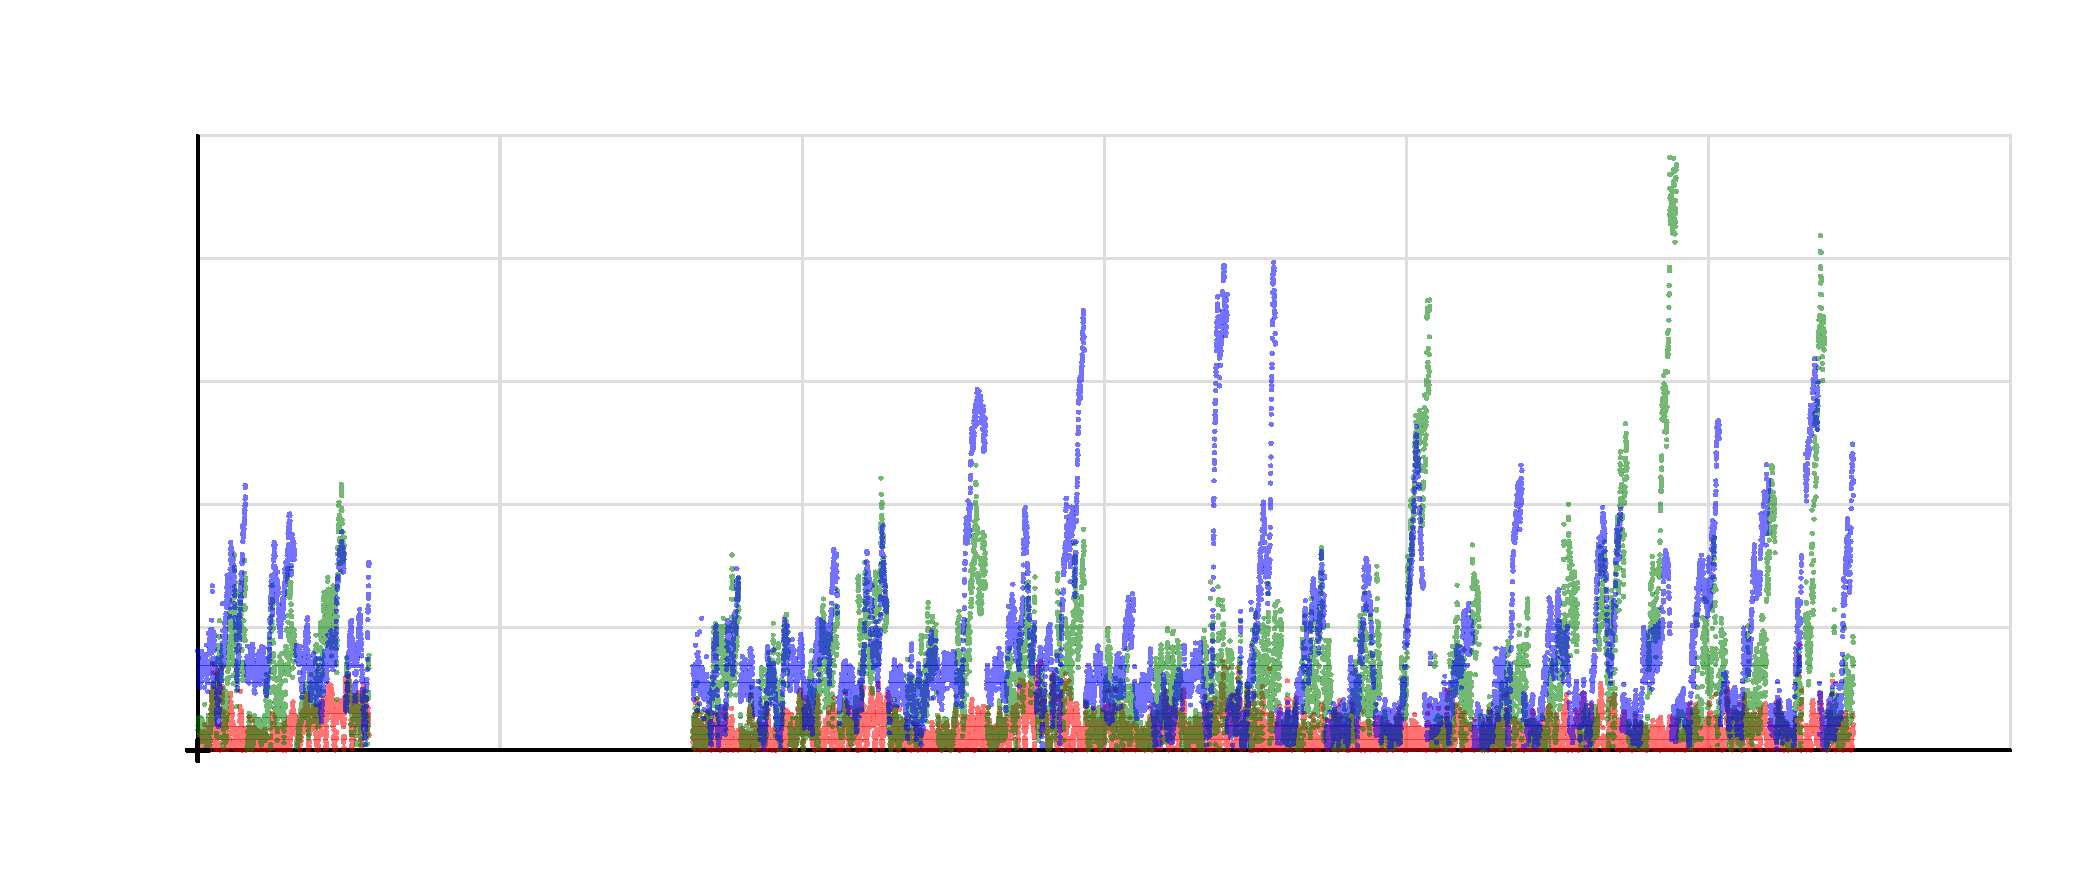
\includegraphics[width=1000.0bp,height=430.0bp]{bericht/abbildungen/horizontal_zeit.pdf}}
\put(95.0,407.0){\makebox(0,0)[lb]{\color{black}\sffamily\fontsize{16}{16}\selectfont Horizontal-Abweichung über der Zeit}}
\put(95.0,50.0){\makebox(0,0)[cb]{\color{black}\sffamily\fontsize{12}{12}\selectfont -10.96}}
\put(87.0,66.0){\makebox(0,0)[rb]{\color{black}\sffamily\fontsize{12}{12}\selectfont -0.007717}}
\put(269.0,50.0){\makebox(0,0)[cb]{\color{black}\sffamily\fontsize{12}{12}\selectfont 48.22}}
\put(87.0,125.0){\makebox(0,0)[rb]{\color{black}\sffamily\fontsize{12}{12}\selectfont 0.01466}}
\put(442.99999999999994,50.0){\makebox(0,0)[cb]{\color{black}\sffamily\fontsize{12}{12}\selectfont 107.4}}
\put(87.0,184.0){\makebox(0,0)[rb]{\color{black}\sffamily\fontsize{12}{12}\selectfont 0.03705}}
\put(617.0000000000001,50.0){\makebox(0,0)[cb]{\color{black}\sffamily\fontsize{12}{12}\selectfont 166.6}}
\put(87.0,243.0){\makebox(0,0)[rb]{\color{black}\sffamily\fontsize{12}{12}\selectfont 0.05943}}
\put(790.9999999999999,50.0){\makebox(0,0)[cb]{\color{black}\sffamily\fontsize{12}{12}\selectfont 225.8}}
\put(87.0,302.0){\makebox(0,0)[rb]{\color{black}\sffamily\fontsize{12}{12}\selectfont 0.08181}}
\put(965.0,50.0){\makebox(0,0)[cb]{\color{black}\sffamily\fontsize{12}{12}\selectfont 284.9}}
\put(87.0,361.0){\makebox(0,0)[rb]{\color{black}\sffamily\fontsize{12}{12}\selectfont 0.1042}}
\put(95.0,385.0){\makebox(0,0)[lb]{\color{red}\sffamily\fontsize{12}{12}\selectfont P23A\_0}}
\put(265.0,385.0){\makebox(0,0)[lb]{\color{green}\sffamily\fontsize{12}{12}\selectfont P23A\_1}}
\put(435.0,385.0){\makebox(0,0)[lb]{\color{blue}\sffamily\fontsize{12}{12}\selectfont UM980}}
\put(530.0,12.0){\makebox(0,0)[cb]{\color{black}\sffamily\fontsize{12}{12}\selectfont Zeit seit gemeinsamem Beginn [min]}}
\put(19.0,217.5){\rotatebox{90}{\makebox(0,0)[b]{\color{black}\sffamily\fontsize{12}{12}\selectfont Horizontal-Abweichung [m]}}}
\end{picture}}
\end{figure}\clearpage
\clearpage\section{English — Turn-table test — 2026-11-03}

Run with Python 3.10 or newer; no additional packages are required:

\begin{quote}\ttfamily\footnotesize python3 turn\_table.py\end{quote}

Open {\small\texttt{ergebnisse/\allowbreak{}index.html}} in a browser. The report contains German, English and Simplified Chinese chapters, each with labelled SVG plots. The SVG files are also available separately. The CSV files contain measured and expected positions, fix quality, correction age, revolutions and east/north errors in metres. {\small\texttt{auswertung.json}} contains fit parameters and statistics. Machine-readable CSV/JSON field names remain unchanged across languages. Keep {\small\texttt{report\_\allowbreak{}languages.py}} alongside {\small\texttt{turn\_\allowbreak{}table.py}}.

To select directories or the maximum reference interpolation gap:

\begin{quote}\ttfamily\footnotesize python3 turn\_table.py --input-dir . --output-dir ergebnisse --max-gap 3\end{quote}

\subsection{Method and time alignment}

NMEA checksums are verified and invalid positions (quality 0) are discarded. Literal {\small\texttt{\textbackslash{}r\textbackslash{}n}} sequences are supported. Time alignment uses the UTC epochs of the GGA messages, rather than file start times or line numbers. Midnight rollovers are detected. The date, 3 November 2026, comes from UM980 RMC messages; the same date is assumed for both P23A files because they contain no date information. An unknown internal measurement latency cannot be independently verified using GGA alone; no subsequent time shift is estimated.

WGS84 latitude/longitude are converted to local east/north coordinates in metres using local WGS84 radii of curvature, which is sufficient for this small measurement area. A geometric circle fit with Huber weights determines the centre and radius from all available RTK-fixed P23A\_0 positions (GGA quality 4).

The reference angle is {\small\texttt{atan2(north-centre\_\allowbreak{}north, east-centre\_\allowbreak{}east)}}, positive from east towards north. The rotation plot shows the relative angle divided by 360° as the number of revolutions since the first reference point, including fractional turns. The CSV files also include this revolution count. The angle is unwrapped over time; a constant rotation rate is not assumed. Radial reference outliers exceeding max(2 cm, 6 robust standard deviations) are excluded from angle determination. No fixed reference points were excluded by this criterion in these data.

Analysis uses the common time interval with available fixed reference data. Where necessary, the unwrapped angle is interpolated between adjacent reliable reference epochs, across no more than {\small\texttt{--max-gap}} seconds. There is no extrapolation. Before the RTK-fixed filter, all three receivers have exactly matching timestamps for the 13,191 time-aligned epochs, so interpolation is unnecessary for these data. After filtering, each receiver retains only its own RTK-fixed epochs; alignment to the reference remains unchanged. Two larger reference gaps are excluded. The number of complete revolutions during these gaps is unknown; the angle resumes at the nearest equivalent angle. Segment numbers are recorded in {\small\texttt{referenz\_\allowbreak{}winkel.csv}}.

For every measurement used:

\begin{quote}\ttfamily\footnotesize expected\_east  = centre\_east  + R*cos(angle(t))\\expected\_north = centre\_north + R*sin(angle(t))\\error         = measured\_position(t) - expected\_position(t)\end{quote}

Only RTK-fixed positions (GGA quality 4) contribute to result CSV files, plots and error statistics. Quality 4 alone does not prove that correction data are currently being received. Outage switching times are therefore not inferred from fix quality or the approximate 3/5-minute cycle. Reported correction ages are included in the CSV files.

Because the expected angle is derived from P23A\_0 itself, its tangential error cannot be determined independently. The red trace mainly shows its radial residual. Systematic errors common to all receivers also cannot be identified under this reference assumption.

\subsection{Results}

Mean rotation period: \textbf{169.599 s} (approximately \textbf{2 min 49.6 s}), the arithmetic mean of \textbf{76 complete revolutions}. Standard deviation: \textbf{15.028 s}; minimum: \textbf{160.797 s}; maximum: \textbf{292.545 s}.

Within each continuous reference segment, successive 360° advances are timed relative to the first angle used. Crossing times are linearly interpolated between adjacent epochs. Each complete revolution has equal weight in the mean. Incomplete turns at segment ends and reference gaps are excluded. Slower motion or stops within a complete turn remain included. Individual durations and segment numbers are saved in {\small\texttt{ergebnisse/\allowbreak{}umdrehungsdauer.csv}}; summary values are also recorded in {\small\texttt{auswertung.json}}.

Radius: \textbf{0.330966 m}. Common analysis interval: \textbf{03:41:09–08:15:08 UTC}, excluding reference gaps.

\begin{center}\small\begin{tabular}{lrrr}\toprule
Receiver & Horizontal RMS & 95th percentile & Maximum\\\midrule
P23A\_0 & 0.00383 m & 0.00769 m & 0.01710 m\\
P23A\_1 & 0.01746 m & 0.03542 m & 0.09647 m\\
UM980 & 0.02071 m & 0.04256 m & 0.07939 m\\
\bottomrule\end{tabular}\end{center}

The full horizontal view shows all RTK-fixed errors. The detail view covers ±10 cm and hides points outside this range. Both axes have equal scales. Red=P23A\_0, green=P23A\_1, blue=UM980, black cross=expected position. Additional plots show revolutions and east, north and horizontal errors over time. Statistics cover all retained epochs, rather than just the detail window or individual outage phases.

Validation included a complete run with all three input files, matching timestamps before the fixed filter and reference alignment after it, a synthetic circle with known centre/radius, a GGA midnight rollover, and the conversion from degrees to revolutions.

\subsection{Outage comparison conclusion}

\textbf{P23A\_1 has smaller typical horizontal errors during periods with stale reference data.} UM980 has the smaller maximum individual error. P23A\_0 receives continuous reference data and is the reference, rather than an outage comparison candidate.

The direct comparison uses 6,812 identical UTC epochs where both receivers are RTK-fixed and both report correction ages >10 s. This is an explicit indicator of stale corrections, not an external log of actual switching times. Non-fixed positions and reference gaps are excluded. The conclusion assesses the accuracy of the remaining fixed solutions, not complete availability throughout all outage phases.

\begin{center}\small\begin{tabular}{lrrrr}\toprule
Receiver & RMS & Median & 95th percentile & Maximum\\\midrule
P23A\_1 & 1.89 cm & 1.30 cm & 3.59 cm & 9.65 cm\\
UM980 & 2.69 cm & 1.90 cm & 5.42 cm & 7.94 cm\\
\bottomrule\end{tabular}\end{center}

P23A\_1 therefore has approximately 30\% lower RMS than UM980 in this comparison. Individual comparison epochs are saved in {\small\texttt{ergebnisse/\allowbreak{}outage\_\allowbreak{}vergleich.csv}}, with summary statistics in {\small\texttt{auswertung.json}}.

\begin{figure}[p]\centering
\resizebox{0.98\linewidth}{!}{%
\setlength{\unitlength}{1bp}\begin{picture}(680.0,680.0)
\put(0,0){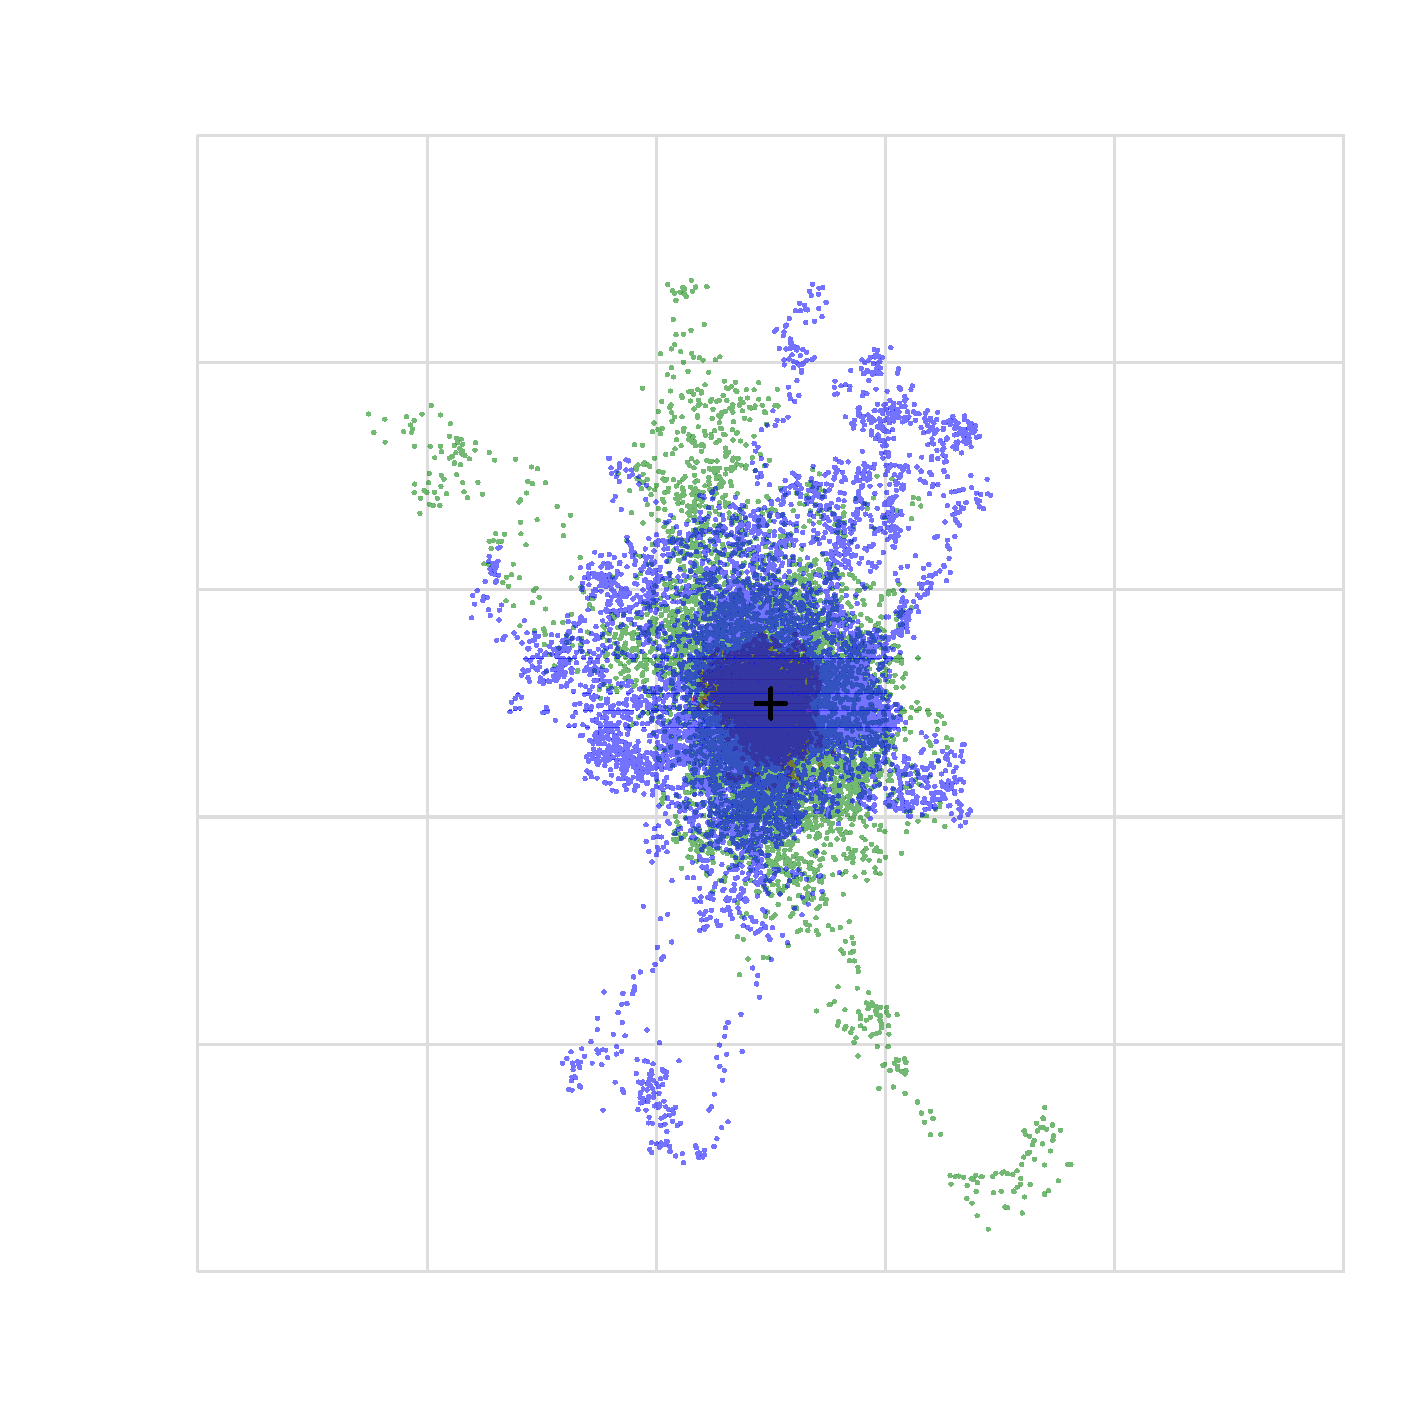
\includegraphics[width=680.0bp,height=680.0bp]{bericht/abbildungen/horizontal_en.pdf}}
\put(95.0,657.0){\makebox(0,0)[lb]{\color{black}\sffamily\fontsize{16}{16}\selectfont Horizontal errors relative to the time-aligned expected circle}}
\put(95.0,50.0){\makebox(0,0)[cb]{\color{black}\sffamily\fontsize{12}{12}\selectfont -0.09642}}
\put(87.0,66.0){\makebox(0,0)[rb]{\color{black}\sffamily\fontsize{12}{12}\selectfont -0.09642}}
\put(205.0,50.0){\makebox(0,0)[cb]{\color{black}\sffamily\fontsize{12}{12}\selectfont -0.05785}}
\put(87.0,175.0){\makebox(0,0)[rb]{\color{black}\sffamily\fontsize{12}{12}\selectfont -0.05785}}
\put(315.0,50.0){\makebox(0,0)[cb]{\color{black}\sffamily\fontsize{12}{12}\selectfont -0.01928}}
\put(87.0,284.0){\makebox(0,0)[rb]{\color{black}\sffamily\fontsize{12}{12}\selectfont -0.01928}}
\put(425.00000000000006,50.0){\makebox(0,0)[cb]{\color{black}\sffamily\fontsize{12}{12}\selectfont 0.01928}}
\put(87.0,393.00000000000006){\makebox(0,0)[rb]{\color{black}\sffamily\fontsize{12}{12}\selectfont 0.01928}}
\put(535.0,50.0){\makebox(0,0)[cb]{\color{black}\sffamily\fontsize{12}{12}\selectfont 0.05785}}
\put(87.0,501.99999999999994){\makebox(0,0)[rb]{\color{black}\sffamily\fontsize{12}{12}\selectfont 0.05785}}
\put(645.0,50.0){\makebox(0,0)[cb]{\color{black}\sffamily\fontsize{12}{12}\selectfont 0.09642}}
\put(87.0,611.0){\makebox(0,0)[rb]{\color{black}\sffamily\fontsize{12}{12}\selectfont 0.09642}}
\put(95.0,635.0){\makebox(0,0)[lb]{\color{red}\sffamily\fontsize{12}{12}\selectfont P23A\_0}}
\put(265.0,635.0){\makebox(0,0)[lb]{\color{green}\sffamily\fontsize{12}{12}\selectfont P23A\_1}}
\put(435.0,635.0){\makebox(0,0)[lb]{\color{blue}\sffamily\fontsize{12}{12}\selectfont UM980}}
\put(379.0,351.5){\makebox(0,0)[lb]{\color{black}\sffamily\fontsize{12}{12}\selectfont Expected (0,0)}}
\put(370.0,12.0){\makebox(0,0)[cb]{\color{black}\sffamily\fontsize{12}{12}\selectfont East error [m]}}
\put(19.0,342.5){\rotatebox{90}{\makebox(0,0)[b]{\color{black}\sffamily\fontsize{12}{12}\selectfont North error [m]}}}
\end{picture}}
\end{figure}
\begin{figure}[p]\centering
\resizebox{0.98\linewidth}{!}{%
\setlength{\unitlength}{1bp}\begin{picture}(680.0,680.0)
\put(0,0){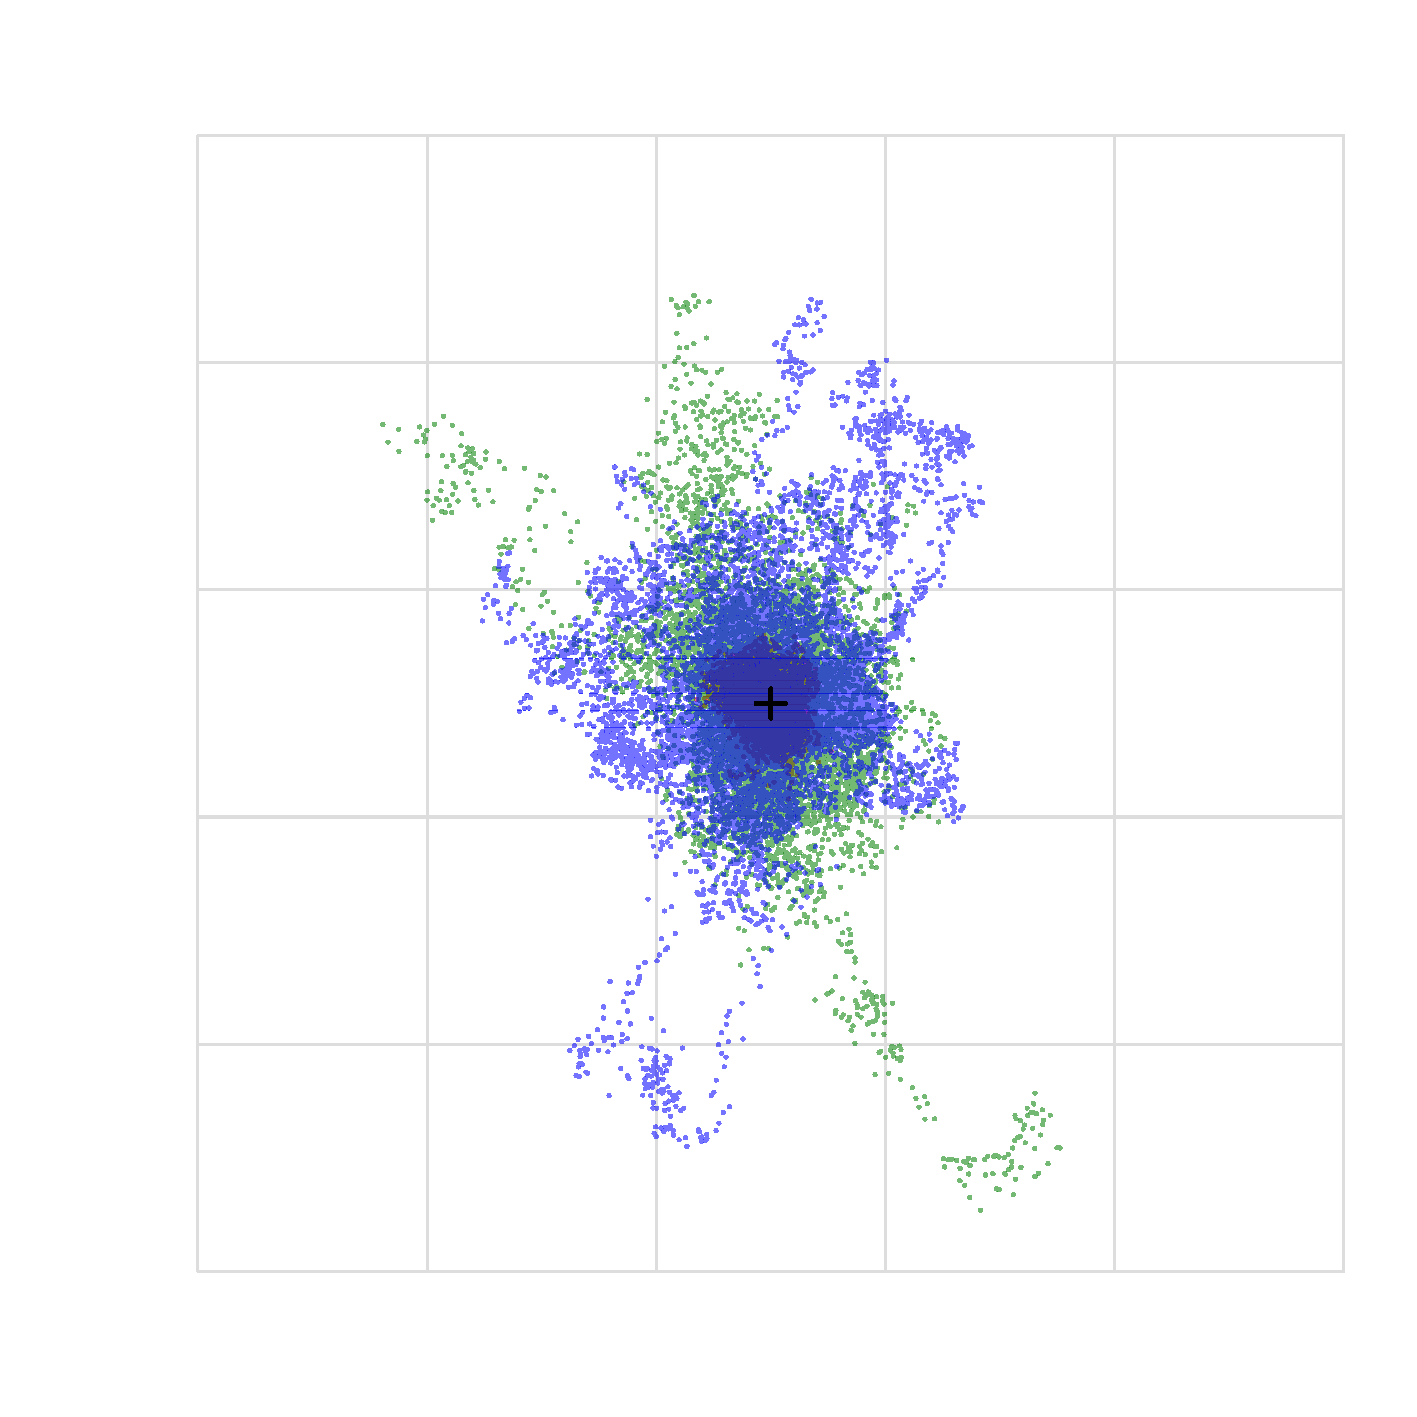
\includegraphics[width=680.0bp,height=680.0bp]{bericht/abbildungen/horizontal_detail_en.pdf}}
\put(95.0,657.0){\makebox(0,0)[lb]{\color{black}\sffamily\fontsize{16}{16}\selectfont Detail ±0.10 m (larger errors hidden)}}
\put(95.0,50.0){\makebox(0,0)[cb]{\color{black}\sffamily\fontsize{12}{12}\selectfont -0.1}}
\put(87.0,66.0){\makebox(0,0)[rb]{\color{black}\sffamily\fontsize{12}{12}\selectfont -0.1}}
\put(205.0,50.0){\makebox(0,0)[cb]{\color{black}\sffamily\fontsize{12}{12}\selectfont -0.06}}
\put(87.0,175.0){\makebox(0,0)[rb]{\color{black}\sffamily\fontsize{12}{12}\selectfont -0.06}}
\put(315.0,50.0){\makebox(0,0)[cb]{\color{black}\sffamily\fontsize{12}{12}\selectfont -0.02}}
\put(87.0,284.0){\makebox(0,0)[rb]{\color{black}\sffamily\fontsize{12}{12}\selectfont -0.02}}
\put(425.00000000000006,50.0){\makebox(0,0)[cb]{\color{black}\sffamily\fontsize{12}{12}\selectfont 0.02}}
\put(87.0,393.00000000000006){\makebox(0,0)[rb]{\color{black}\sffamily\fontsize{12}{12}\selectfont 0.02}}
\put(535.0,50.0){\makebox(0,0)[cb]{\color{black}\sffamily\fontsize{12}{12}\selectfont 0.06}}
\put(87.0,501.99999999999994){\makebox(0,0)[rb]{\color{black}\sffamily\fontsize{12}{12}\selectfont 0.06}}
\put(645.0,50.0){\makebox(0,0)[cb]{\color{black}\sffamily\fontsize{12}{12}\selectfont 0.1}}
\put(87.0,611.0){\makebox(0,0)[rb]{\color{black}\sffamily\fontsize{12}{12}\selectfont 0.1}}
\put(95.0,635.0){\makebox(0,0)[lb]{\color{red}\sffamily\fontsize{12}{12}\selectfont P23A\_0}}
\put(265.0,635.0){\makebox(0,0)[lb]{\color{green}\sffamily\fontsize{12}{12}\selectfont P23A\_1}}
\put(435.0,635.0){\makebox(0,0)[lb]{\color{blue}\sffamily\fontsize{12}{12}\selectfont UM980}}
\put(379.0,351.5){\makebox(0,0)[lb]{\color{black}\sffamily\fontsize{12}{12}\selectfont Expected (0,0)}}
\put(370.0,12.0){\makebox(0,0)[cb]{\color{black}\sffamily\fontsize{12}{12}\selectfont East error [m]}}
\put(19.0,342.5){\rotatebox{90}{\makebox(0,0)[b]{\color{black}\sffamily\fontsize{12}{12}\selectfont North error [m]}}}
\end{picture}}
\end{figure}
\begin{figure}[p]\centering
\resizebox{0.98\linewidth}{!}{%
\setlength{\unitlength}{1bp}\begin{picture}(1000.0,430.0)
\put(0,0){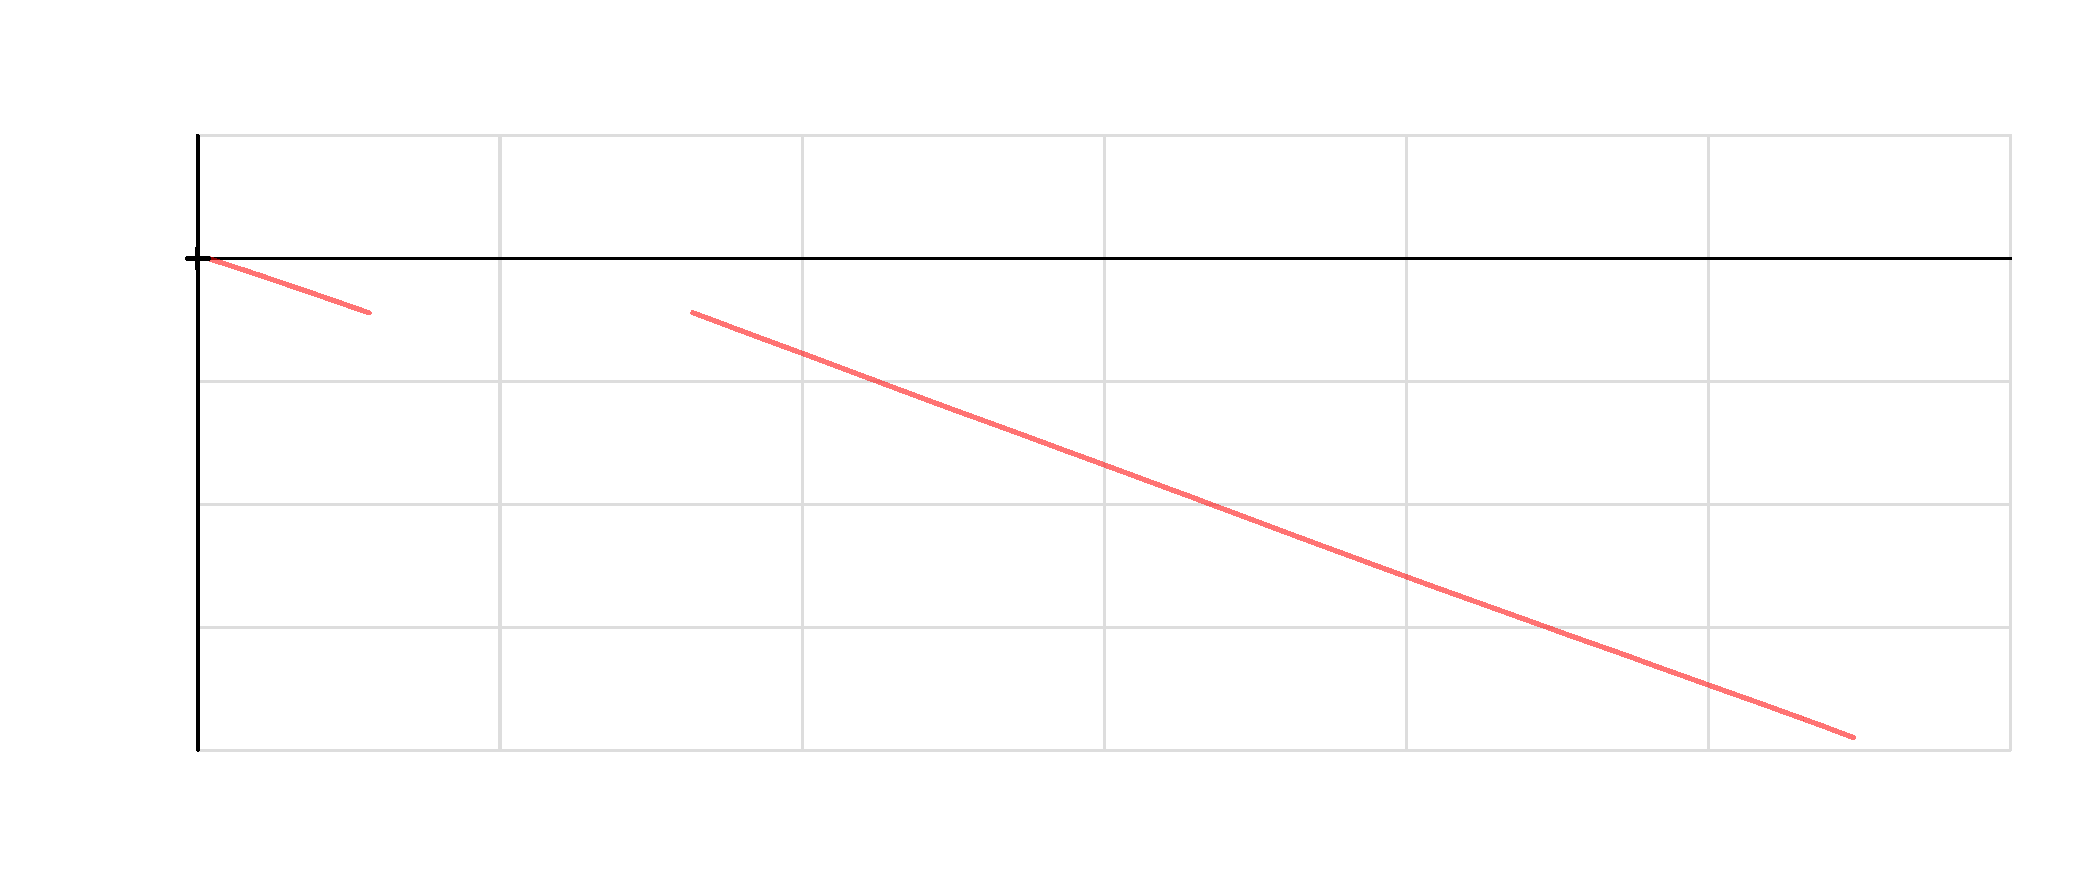
\includegraphics[width=1000.0bp,height=430.0bp]{bericht/abbildungen/winkel_en.pdf}}
\put(95.0,407.0){\makebox(0,0)[lb]{\color{black}\sffamily\fontsize{16}{16}\selectfont Revolutions: positive from east towards north}}
\put(95.0,50.0){\makebox(0,0)[cb]{\color{black}\sffamily\fontsize{12}{12}\selectfont -10.96}}
\put(87.0,66.0){\makebox(0,0)[rb]{\color{black}\sffamily\fontsize{12}{12}\selectfont -84.19}}
\put(269.0,50.0){\makebox(0,0)[cb]{\color{black}\sffamily\fontsize{12}{12}\selectfont 48.22}}
\put(87.0,125.0){\makebox(0,0)[rb]{\color{black}\sffamily\fontsize{12}{12}\selectfont -66.1}}
\put(442.99999999999994,50.0){\makebox(0,0)[cb]{\color{black}\sffamily\fontsize{12}{12}\selectfont 107.4}}
\put(87.0,184.0){\makebox(0,0)[rb]{\color{black}\sffamily\fontsize{12}{12}\selectfont -48.02}}
\put(617.0000000000001,50.0){\makebox(0,0)[cb]{\color{black}\sffamily\fontsize{12}{12}\selectfont 166.6}}
\put(87.0,243.00000000000003){\makebox(0,0)[rb]{\color{black}\sffamily\fontsize{12}{12}\selectfont -29.93}}
\put(790.9999999999999,50.0){\makebox(0,0)[cb]{\color{black}\sffamily\fontsize{12}{12}\selectfont 225.8}}
\put(87.0,302.0){\makebox(0,0)[rb]{\color{black}\sffamily\fontsize{12}{12}\selectfont -11.85}}
\put(965.0,50.0){\makebox(0,0)[cb]{\color{black}\sffamily\fontsize{12}{12}\selectfont 284.9}}
\put(87.0,361.0){\makebox(0,0)[rb]{\color{black}\sffamily\fontsize{12}{12}\selectfont 6.24}}
\put(95.0,385.0){\makebox(0,0)[lb]{\color{red}\sffamily\fontsize{12}{12}\selectfont P23A\_0}}
\put(530.0,12.0){\makebox(0,0)[cb]{\color{black}\sffamily\fontsize{12}{12}\selectfont Time since common start [min]}}
\put(19.0,217.5){\rotatebox{90}{\makebox(0,0)[b]{\color{black}\sffamily\fontsize{12}{12}\selectfont Revolutions since first reference point}}}
\end{picture}}
\end{figure}
\begin{figure}[p]\centering
\resizebox{0.98\linewidth}{!}{%
\setlength{\unitlength}{1bp}\begin{picture}(1000.0,430.0)
\put(0,0){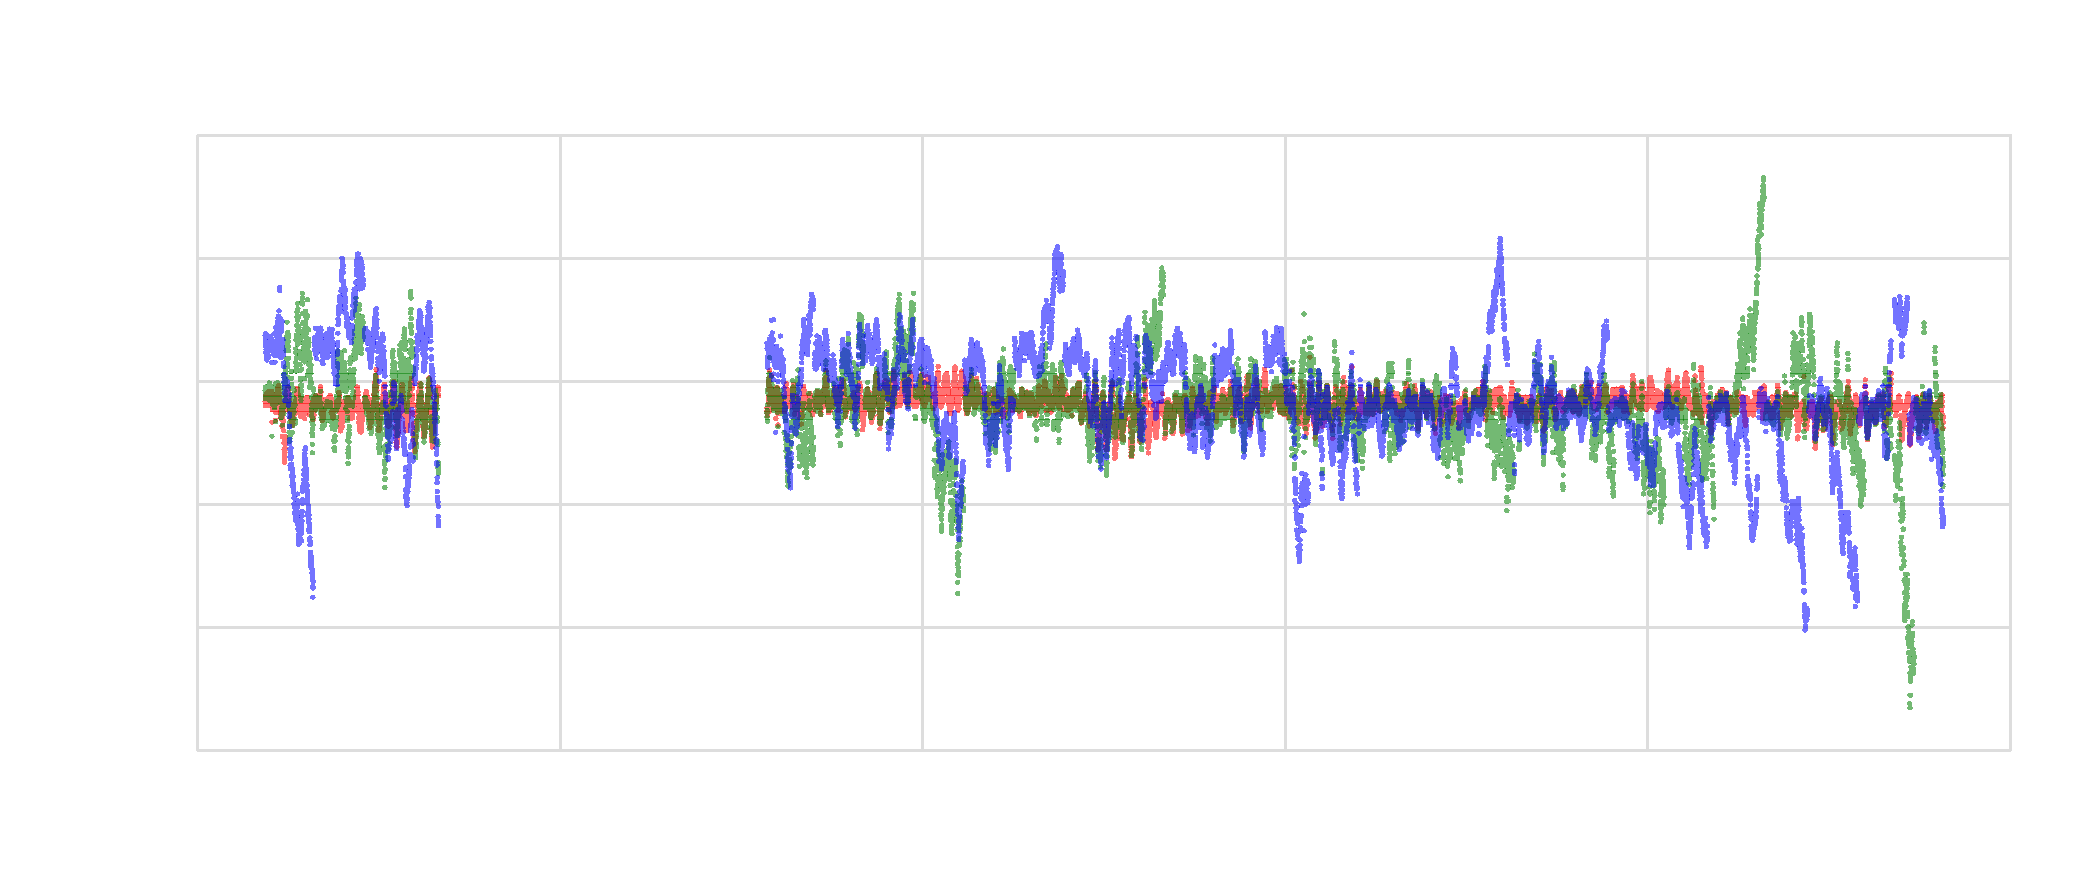
\includegraphics[width=1000.0bp,height=430.0bp]{bericht/abbildungen/east_zeit_en.pdf}}
\put(95.0,407.0){\makebox(0,0)[lb]{\color{black}\sffamily\fontsize{16}{16}\selectfont East error over time}}
\put(95.0,50.0){\makebox(0,0)[cb]{\color{black}\sffamily\fontsize{12}{12}\selectfont -10.96}}
\put(87.0,66.0){\makebox(0,0)[rb]{\color{black}\sffamily\fontsize{12}{12}\selectfont -0.0772}}
\put(269.0,50.0){\makebox(0,0)[cb]{\color{black}\sffamily\fontsize{12}{12}\selectfont 48.22}}
\put(87.0,125.0){\makebox(0,0)[rb]{\color{black}\sffamily\fontsize{12}{12}\selectfont -0.04977}}
\put(442.99999999999994,50.0){\makebox(0,0)[cb]{\color{black}\sffamily\fontsize{12}{12}\selectfont 107.4}}
\put(87.0,184.0){\makebox(0,0)[rb]{\color{black}\sffamily\fontsize{12}{12}\selectfont -0.02235}}
\put(617.0000000000001,50.0){\makebox(0,0)[cb]{\color{black}\sffamily\fontsize{12}{12}\selectfont 166.6}}
\put(87.0,243.0){\makebox(0,0)[rb]{\color{black}\sffamily\fontsize{12}{12}\selectfont 0.005077}}
\put(790.9999999999999,50.0){\makebox(0,0)[cb]{\color{black}\sffamily\fontsize{12}{12}\selectfont 225.8}}
\put(87.0,302.0){\makebox(0,0)[rb]{\color{black}\sffamily\fontsize{12}{12}\selectfont 0.0325}}
\put(965.0,50.0){\makebox(0,0)[cb]{\color{black}\sffamily\fontsize{12}{12}\selectfont 284.9}}
\put(87.0,361.0){\makebox(0,0)[rb]{\color{black}\sffamily\fontsize{12}{12}\selectfont 0.05993}}
\put(95.0,385.0){\makebox(0,0)[lb]{\color{red}\sffamily\fontsize{12}{12}\selectfont P23A\_0}}
\put(265.0,385.0){\makebox(0,0)[lb]{\color{green}\sffamily\fontsize{12}{12}\selectfont P23A\_1}}
\put(435.0,385.0){\makebox(0,0)[lb]{\color{blue}\sffamily\fontsize{12}{12}\selectfont UM980}}
\put(530.0,12.0){\makebox(0,0)[cb]{\color{black}\sffamily\fontsize{12}{12}\selectfont Time since common start [min]}}
\put(19.0,217.5){\rotatebox{90}{\makebox(0,0)[b]{\color{black}\sffamily\fontsize{12}{12}\selectfont East error [m]}}}
\end{picture}}
\end{figure}
\begin{figure}[p]\centering
\resizebox{0.98\linewidth}{!}{%
\setlength{\unitlength}{1bp}\begin{picture}(1000.0,430.0)
\put(0,0){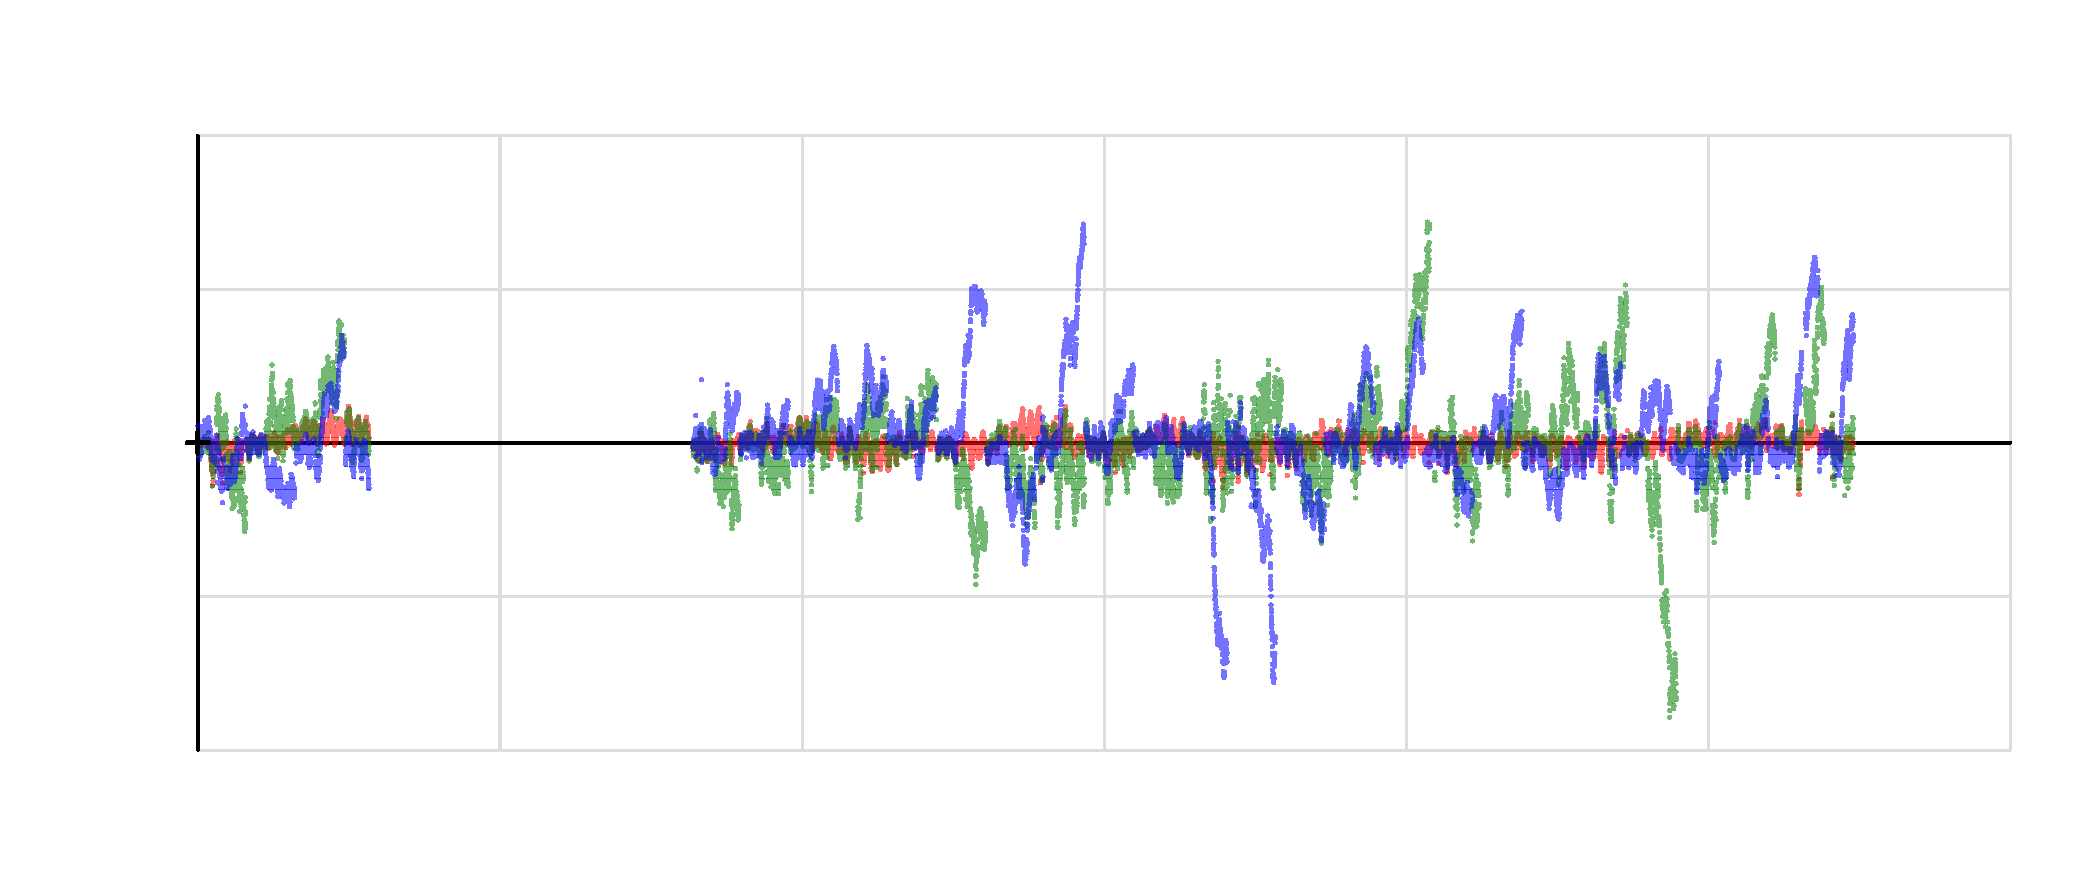
\includegraphics[width=1000.0bp,height=430.0bp]{bericht/abbildungen/north_zeit_en.pdf}}
\put(95.0,407.0){\makebox(0,0)[lb]{\color{black}\sffamily\fontsize{16}{16}\selectfont North error over time}}
\put(95.0,50.0){\makebox(0,0)[cb]{\color{black}\sffamily\fontsize{12}{12}\selectfont -10.96}}
\put(87.0,66.0){\makebox(0,0)[rb]{\color{black}\sffamily\fontsize{12}{12}\selectfont -0.1022}}
\put(269.0,50.0){\makebox(0,0)[cb]{\color{black}\sffamily\fontsize{12}{12}\selectfont 48.22}}
\put(87.0,125.0){\makebox(0,0)[rb]{\color{black}\sffamily\fontsize{12}{12}\selectfont -0.06478}}
\put(442.99999999999994,50.0){\makebox(0,0)[cb]{\color{black}\sffamily\fontsize{12}{12}\selectfont 107.4}}
\put(87.0,184.0){\makebox(0,0)[rb]{\color{black}\sffamily\fontsize{12}{12}\selectfont -0.0274}}
\put(617.0000000000001,50.0){\makebox(0,0)[cb]{\color{black}\sffamily\fontsize{12}{12}\selectfont 166.6}}
\put(87.0,243.0){\makebox(0,0)[rb]{\color{black}\sffamily\fontsize{12}{12}\selectfont 0.00999}}
\put(790.9999999999999,50.0){\makebox(0,0)[cb]{\color{black}\sffamily\fontsize{12}{12}\selectfont 225.8}}
\put(87.0,302.0){\makebox(0,0)[rb]{\color{black}\sffamily\fontsize{12}{12}\selectfont 0.04738}}
\put(965.0,50.0){\makebox(0,0)[cb]{\color{black}\sffamily\fontsize{12}{12}\selectfont 284.9}}
\put(87.0,361.0){\makebox(0,0)[rb]{\color{black}\sffamily\fontsize{12}{12}\selectfont 0.08476}}
\put(95.0,385.0){\makebox(0,0)[lb]{\color{red}\sffamily\fontsize{12}{12}\selectfont P23A\_0}}
\put(265.0,385.0){\makebox(0,0)[lb]{\color{green}\sffamily\fontsize{12}{12}\selectfont P23A\_1}}
\put(435.0,385.0){\makebox(0,0)[lb]{\color{blue}\sffamily\fontsize{12}{12}\selectfont UM980}}
\put(530.0,12.0){\makebox(0,0)[cb]{\color{black}\sffamily\fontsize{12}{12}\selectfont Time since common start [min]}}
\put(19.0,217.5){\rotatebox{90}{\makebox(0,0)[b]{\color{black}\sffamily\fontsize{12}{12}\selectfont North error [m]}}}
\end{picture}}
\end{figure}
\begin{figure}[p]\centering
\resizebox{0.98\linewidth}{!}{%
\setlength{\unitlength}{1bp}\begin{picture}(1000.0,430.0)
\put(0,0){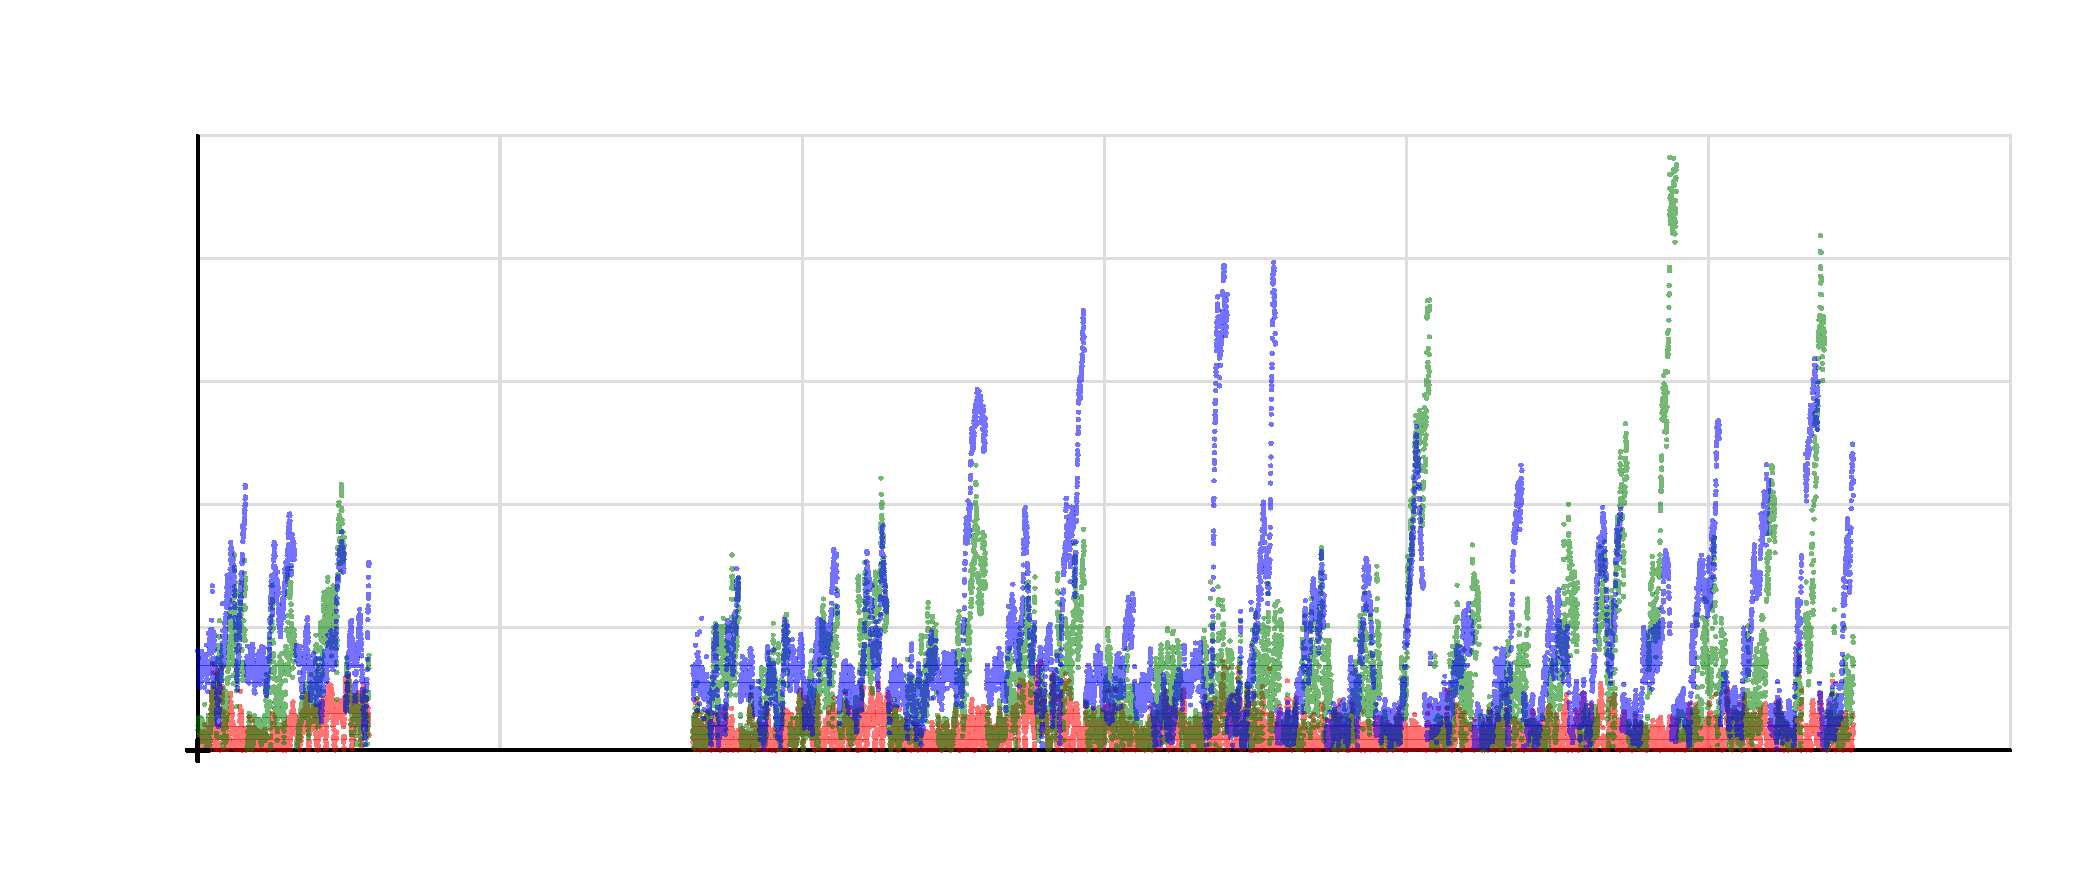
\includegraphics[width=1000.0bp,height=430.0bp]{bericht/abbildungen/horizontal_zeit_en.pdf}}
\put(95.0,407.0){\makebox(0,0)[lb]{\color{black}\sffamily\fontsize{16}{16}\selectfont Horizontal error over time}}
\put(95.0,50.0){\makebox(0,0)[cb]{\color{black}\sffamily\fontsize{12}{12}\selectfont -10.96}}
\put(87.0,66.0){\makebox(0,0)[rb]{\color{black}\sffamily\fontsize{12}{12}\selectfont -0.007717}}
\put(269.0,50.0){\makebox(0,0)[cb]{\color{black}\sffamily\fontsize{12}{12}\selectfont 48.22}}
\put(87.0,125.0){\makebox(0,0)[rb]{\color{black}\sffamily\fontsize{12}{12}\selectfont 0.01466}}
\put(442.99999999999994,50.0){\makebox(0,0)[cb]{\color{black}\sffamily\fontsize{12}{12}\selectfont 107.4}}
\put(87.0,184.0){\makebox(0,0)[rb]{\color{black}\sffamily\fontsize{12}{12}\selectfont 0.03705}}
\put(617.0000000000001,50.0){\makebox(0,0)[cb]{\color{black}\sffamily\fontsize{12}{12}\selectfont 166.6}}
\put(87.0,243.0){\makebox(0,0)[rb]{\color{black}\sffamily\fontsize{12}{12}\selectfont 0.05943}}
\put(790.9999999999999,50.0){\makebox(0,0)[cb]{\color{black}\sffamily\fontsize{12}{12}\selectfont 225.8}}
\put(87.0,302.0){\makebox(0,0)[rb]{\color{black}\sffamily\fontsize{12}{12}\selectfont 0.08181}}
\put(965.0,50.0){\makebox(0,0)[cb]{\color{black}\sffamily\fontsize{12}{12}\selectfont 284.9}}
\put(87.0,361.0){\makebox(0,0)[rb]{\color{black}\sffamily\fontsize{12}{12}\selectfont 0.1042}}
\put(95.0,385.0){\makebox(0,0)[lb]{\color{red}\sffamily\fontsize{12}{12}\selectfont P23A\_0}}
\put(265.0,385.0){\makebox(0,0)[lb]{\color{green}\sffamily\fontsize{12}{12}\selectfont P23A\_1}}
\put(435.0,385.0){\makebox(0,0)[lb]{\color{blue}\sffamily\fontsize{12}{12}\selectfont UM980}}
\put(530.0,12.0){\makebox(0,0)[cb]{\color{black}\sffamily\fontsize{12}{12}\selectfont Time since common start [min]}}
\put(19.0,217.5){\rotatebox{90}{\makebox(0,0)[b]{\color{black}\sffamily\fontsize{12}{12}\selectfont Horizontal error [m]}}}
\end{picture}}
\end{figure}\clearpage
\clearpage\section{{\cjkfont 中}\allowbreak{}{\cjkfont 文}\allowbreak{}{\cjkfont （}\allowbreak{}{\cjkfont 简}\allowbreak{}{\cjkfont 体}\allowbreak{}{\cjkfont ）}\allowbreak{}— {\cjkfont 转}\allowbreak{}{\cjkfont 台}\allowbreak{}{\cjkfont 测}\allowbreak{}{\cjkfont 试}\allowbreak{} — 2026{\cjkfont 年}\allowbreak{}11{\cjkfont 月}\allowbreak{}3{\cjkfont 日}\allowbreak{}}

{\cjkfont 运}\allowbreak{}{\cjkfont 行}\allowbreak{}{\cjkfont 环}\allowbreak{}{\cjkfont 境}\allowbreak{}{\cjkfont 为}\allowbreak{} Python 3.10 {\cjkfont 或}\allowbreak{}{\cjkfont 更}\allowbreak{}{\cjkfont 新}\allowbreak{}{\cjkfont 版}\allowbreak{}{\cjkfont 本}\allowbreak{}{\cjkfont ，}\allowbreak{}{\cjkfont 无}\allowbreak{}{\cjkfont 需}\allowbreak{}{\cjkfont 安}\allowbreak{}{\cjkfont 装}\allowbreak{}{\cjkfont 额}\allowbreak{}{\cjkfont 外}\allowbreak{}{\cjkfont 软}\allowbreak{}{\cjkfont 件}\allowbreak{}{\cjkfont 包}\allowbreak{}{\cjkfont ：}\allowbreak{}

\begin{quote}\ttfamily\footnotesize python3 turn\_table.py\end{quote}

{\cjkfont 在}\allowbreak{}{\cjkfont 浏}\allowbreak{}{\cjkfont 览}\allowbreak{}{\cjkfont 器}\allowbreak{}{\cjkfont 中}\allowbreak{}{\cjkfont 打}\allowbreak{}{\cjkfont 开}\allowbreak{} {\small\texttt{ergebnisse/\allowbreak{}index.html}}{\cjkfont 。}\allowbreak{}{\cjkfont 报}\allowbreak{}{\cjkfont 告}\allowbreak{}{\cjkfont 依}\allowbreak{}{\cjkfont 次}\allowbreak{}{\cjkfont 包}\allowbreak{}{\cjkfont 含}\allowbreak{}{\cjkfont 德}\allowbreak{}{\cjkfont 文}\allowbreak{}{\cjkfont 、}\allowbreak{}{\cjkfont 英}\allowbreak{}{\cjkfont 文}\allowbreak{}{\cjkfont 和}\allowbreak{}{\cjkfont 简}\allowbreak{}{\cjkfont 体}\allowbreak{}{\cjkfont 中}\allowbreak{}{\cjkfont 文}\allowbreak{}{\cjkfont 章}\allowbreak{}{\cjkfont 节}\allowbreak{}{\cjkfont ，}\allowbreak{}{\cjkfont 每}\allowbreak{}{\cjkfont 个}\allowbreak{}{\cjkfont 章}\allowbreak{}{\cjkfont 节}\allowbreak{}{\cjkfont 均}\allowbreak{}{\cjkfont 配}\allowbreak{}{\cjkfont 有}\allowbreak{}{\cjkfont 相}\allowbreak{}{\cjkfont 应}\allowbreak{}{\cjkfont 语}\allowbreak{}{\cjkfont 言}\allowbreak{}{\cjkfont 标}\allowbreak{}{\cjkfont 注}\allowbreak{}{\cjkfont 的}\allowbreak{} SVG {\cjkfont 图}\allowbreak{}{\cjkfont 。}\allowbreak{}{\cjkfont 各}\allowbreak{} SVG {\cjkfont 图}\allowbreak{}{\cjkfont 也}\allowbreak{}{\cjkfont 可}\allowbreak{}{\cjkfont 单}\allowbreak{}{\cjkfont 独}\allowbreak{}{\cjkfont 打}\allowbreak{}{\cjkfont 开}\allowbreak{}{\cjkfont 。}\allowbreak{}CSV {\cjkfont 文}\allowbreak{}{\cjkfont 件}\allowbreak{}{\cjkfont 包}\allowbreak{}{\cjkfont 含}\allowbreak{}{\cjkfont 实}\allowbreak{}{\cjkfont 测}\allowbreak{}{\cjkfont 位}\allowbreak{}{\cjkfont 置}\allowbreak{}{\cjkfont 、}\allowbreak{}{\cjkfont 理}\allowbreak{}{\cjkfont 论}\allowbreak{}{\cjkfont 位}\allowbreak{}{\cjkfont 置}\allowbreak{}{\cjkfont 、}\allowbreak{}{\cjkfont 定}\allowbreak{}{\cjkfont 位}\allowbreak{}{\cjkfont 解}\allowbreak{}{\cjkfont 质}\allowbreak{}{\cjkfont 量}\allowbreak{}{\cjkfont 、}\allowbreak{}{\cjkfont 差}\allowbreak{}{\cjkfont 分}\allowbreak{}{\cjkfont 改}\allowbreak{}{\cjkfont 正}\allowbreak{}{\cjkfont 数}\allowbreak{}{\cjkfont 据}\allowbreak{}{\cjkfont 龄}\allowbreak{}{\cjkfont 期}\allowbreak{}{\cjkfont 、}\allowbreak{}{\cjkfont 旋}\allowbreak{}{\cjkfont 转}\allowbreak{}{\cjkfont 圈}\allowbreak{}{\cjkfont 数}\allowbreak{}{\cjkfont 以}\allowbreak{}{\cjkfont 及}\allowbreak{}{\cjkfont 以}\allowbreak{}{\cjkfont 米}\allowbreak{}{\cjkfont 为}\allowbreak{}{\cjkfont 单}\allowbreak{}{\cjkfont 位}\allowbreak{}{\cjkfont 的}\allowbreak{}{\cjkfont 东}\allowbreak{}{\cjkfont 向}\allowbreak{}{\cjkfont 和}\allowbreak{}{\cjkfont 北}\allowbreak{}{\cjkfont 向}\allowbreak{}{\cjkfont 误}\allowbreak{}{\cjkfont 差}\allowbreak{}{\cjkfont 。}\allowbreak{}{\small\texttt{auswertung.json}} {\cjkfont 包}\allowbreak{}{\cjkfont 含}\allowbreak{}{\cjkfont 拟}\allowbreak{}{\cjkfont 合}\allowbreak{}{\cjkfont 参}\allowbreak{}{\cjkfont 数}\allowbreak{}{\cjkfont 和}\allowbreak{}{\cjkfont 统}\allowbreak{}{\cjkfont 计}\allowbreak{}{\cjkfont 结}\allowbreak{}{\cjkfont 果}\allowbreak{}{\cjkfont 。}\allowbreak{}CSV/JSON {\cjkfont 的}\allowbreak{}{\cjkfont 机}\allowbreak{}{\cjkfont 器}\allowbreak{}{\cjkfont 可}\allowbreak{}{\cjkfont 读}\allowbreak{}{\cjkfont 字}\allowbreak{}{\cjkfont 段}\allowbreak{}{\cjkfont 名}\allowbreak{}{\cjkfont 不}\allowbreak{}{\cjkfont 随}\allowbreak{}{\cjkfont 报}\allowbreak{}{\cjkfont 告}\allowbreak{}{\cjkfont 语}\allowbreak{}{\cjkfont 言}\allowbreak{}{\cjkfont 改}\allowbreak{}{\cjkfont 变}\allowbreak{}{\cjkfont 。}\allowbreak{}{\cjkfont 请}\allowbreak{}{\cjkfont 将}\allowbreak{} {\small\texttt{report\_\allowbreak{}languages.py}} {\cjkfont 与}\allowbreak{} {\small\texttt{turn\_\allowbreak{}table.py}} {\cjkfont 放}\allowbreak{}{\cjkfont 在}\allowbreak{}{\cjkfont 同}\allowbreak{}{\cjkfont 一}\allowbreak{}{\cjkfont 目}\allowbreak{}{\cjkfont 录}\allowbreak{}{\cjkfont 中}\allowbreak{}{\cjkfont 。}\allowbreak{}

{\cjkfont 如}\allowbreak{}{\cjkfont 需}\allowbreak{}{\cjkfont 指}\allowbreak{}{\cjkfont 定}\allowbreak{}{\cjkfont 目}\allowbreak{}{\cjkfont 录}\allowbreak{}{\cjkfont 或}\allowbreak{}{\cjkfont 参}\allowbreak{}{\cjkfont 考}\allowbreak{}{\cjkfont 数}\allowbreak{}{\cjkfont 据}\allowbreak{}{\cjkfont 插}\allowbreak{}{\cjkfont 值}\allowbreak{}{\cjkfont 所}\allowbreak{}{\cjkfont 允}\allowbreak{}{\cjkfont 许}\allowbreak{}{\cjkfont 的}\allowbreak{}{\cjkfont 最}\allowbreak{}{\cjkfont 大}\allowbreak{}{\cjkfont 时}\allowbreak{}{\cjkfont 间}\allowbreak{}{\cjkfont 间}\allowbreak{}{\cjkfont 隔}\allowbreak{}{\cjkfont ：}\allowbreak{}

\begin{quote}\ttfamily\footnotesize python3 turn\_table.py --input-dir . --output-dir ergebnisse --max-gap 3\end{quote}

\subsection{{\cjkfont 方}\allowbreak{}{\cjkfont 法}\allowbreak{}{\cjkfont 与}\allowbreak{}{\cjkfont 时}\allowbreak{}{\cjkfont 间}\allowbreak{}{\cjkfont 对}\allowbreak{}{\cjkfont 齐}\allowbreak{}}

{\cjkfont 程}\allowbreak{}{\cjkfont 序}\allowbreak{}{\cjkfont 验}\allowbreak{}{\cjkfont 证}\allowbreak{} NMEA {\cjkfont 校}\allowbreak{}{\cjkfont 验}\allowbreak{}{\cjkfont 和}\allowbreak{}{\cjkfont ，}\allowbreak{}{\cjkfont 并}\allowbreak{}{\cjkfont 丢}\allowbreak{}{\cjkfont 弃}\allowbreak{}{\cjkfont 无}\allowbreak{}{\cjkfont 效}\allowbreak{}{\cjkfont 位}\allowbreak{}{\cjkfont 置}\allowbreak{}{\cjkfont （}\allowbreak{}{\cjkfont 质}\allowbreak{}{\cjkfont 量}\allowbreak{}{\cjkfont 标}\allowbreak{}{\cjkfont 识}\allowbreak{}{\cjkfont 为}\allowbreak{} 0{\cjkfont ）}\allowbreak{}{\cjkfont 。}\allowbreak{}{\cjkfont 同}\allowbreak{}{\cjkfont 时}\allowbreak{}{\cjkfont 支}\allowbreak{}{\cjkfont 持}\allowbreak{}{\cjkfont 以}\allowbreak{}{\cjkfont 字}\allowbreak{}{\cjkfont 面}\allowbreak{}{\cjkfont 字}\allowbreak{}{\cjkfont 符}\allowbreak{}{\cjkfont 形}\allowbreak{}{\cjkfont 式}\allowbreak{}{\cjkfont 保}\allowbreak{}{\cjkfont 存}\allowbreak{}{\cjkfont 的}\allowbreak{} {\small\texttt{\textbackslash{}r\textbackslash{}n}}{\cjkfont 。}\allowbreak{}{\cjkfont 时}\allowbreak{}{\cjkfont 间}\allowbreak{}{\cjkfont 对}\allowbreak{}{\cjkfont 齐}\allowbreak{}{\cjkfont 采}\allowbreak{}{\cjkfont 用}\allowbreak{} GGA {\cjkfont 消}\allowbreak{}{\cjkfont 息}\allowbreak{}{\cjkfont 中}\allowbreak{}{\cjkfont 的}\allowbreak{} UTC {\cjkfont 历}\allowbreak{}{\cjkfont 元}\allowbreak{}{\cjkfont ，}\allowbreak{}{\cjkfont 而}\allowbreak{}{\cjkfont 非}\allowbreak{}{\cjkfont 文}\allowbreak{}{\cjkfont 件}\allowbreak{}{\cjkfont 起}\allowbreak{}{\cjkfont 始}\allowbreak{}{\cjkfont 时}\allowbreak{}{\cjkfont 间}\allowbreak{}{\cjkfont 或}\allowbreak{}{\cjkfont 行}\allowbreak{}{\cjkfont 号}\allowbreak{}{\cjkfont 。}\allowbreak{}{\cjkfont 程}\allowbreak{}{\cjkfont 序}\allowbreak{}{\cjkfont 可}\allowbreak{}{\cjkfont 识}\allowbreak{}{\cjkfont 别}\allowbreak{}{\cjkfont 跨}\allowbreak{}{\cjkfont 越}\allowbreak{}{\cjkfont 午}\allowbreak{}{\cjkfont 夜}\allowbreak{}{\cjkfont 的}\allowbreak{}{\cjkfont 情}\allowbreak{}{\cjkfont 况}\allowbreak{}{\cjkfont 。}\allowbreak{}{\cjkfont 日}\allowbreak{}{\cjkfont 期}\allowbreak{} 2026 {\cjkfont 年}\allowbreak{} 11 {\cjkfont 月}\allowbreak{} 3 {\cjkfont 日}\allowbreak{}{\cjkfont 来}\allowbreak{}{\cjkfont 自}\allowbreak{} UM980 {\cjkfont 的}\allowbreak{} RMC {\cjkfont 消}\allowbreak{}{\cjkfont 息}\allowbreak{}{\cjkfont ；}\allowbreak{}{\cjkfont 由}\allowbreak{}{\cjkfont 于}\allowbreak{}{\cjkfont 两}\allowbreak{}{\cjkfont 份}\allowbreak{} P23A {\cjkfont 文}\allowbreak{}{\cjkfont 件}\allowbreak{}{\cjkfont 不}\allowbreak{}{\cjkfont 含}\allowbreak{}{\cjkfont 日}\allowbreak{}{\cjkfont 期}\allowbreak{}{\cjkfont 信}\allowbreak{}{\cjkfont 息}\allowbreak{}{\cjkfont ，}\allowbreak{}{\cjkfont 假}\allowbreak{}{\cjkfont 定}\allowbreak{}{\cjkfont 其}\allowbreak{}{\cjkfont 采}\allowbreak{}{\cjkfont 集}\allowbreak{}{\cjkfont 于}\allowbreak{}{\cjkfont 同}\allowbreak{}{\cjkfont 一}\allowbreak{}{\cjkfont 天}\allowbreak{}{\cjkfont 。}\allowbreak{}{\cjkfont 仅}\allowbreak{}{\cjkfont 凭}\allowbreak{} GGA {\cjkfont 无}\allowbreak{}{\cjkfont 法}\allowbreak{}{\cjkfont 独}\allowbreak{}{\cjkfont 立}\allowbreak{}{\cjkfont 验}\allowbreak{}{\cjkfont 证}\allowbreak{}{\cjkfont 未}\allowbreak{}{\cjkfont 知}\allowbreak{}{\cjkfont 的}\allowbreak{}{\cjkfont 接}\allowbreak{}{\cjkfont 收}\allowbreak{}{\cjkfont 机}\allowbreak{}{\cjkfont 内}\allowbreak{}{\cjkfont 部}\allowbreak{}{\cjkfont 测}\allowbreak{}{\cjkfont 量}\allowbreak{}{\cjkfont 延}\allowbreak{}{\cjkfont 迟}\allowbreak{}{\cjkfont ，}\allowbreak{}{\cjkfont 因}\allowbreak{}{\cjkfont 此}\allowbreak{}{\cjkfont 不}\allowbreak{}{\cjkfont 估}\allowbreak{}{\cjkfont 计}\allowbreak{}{\cjkfont 或}\allowbreak{}{\cjkfont 施}\allowbreak{}{\cjkfont 加}\allowbreak{}{\cjkfont 事}\allowbreak{}{\cjkfont 后}\allowbreak{}{\cjkfont 时}\allowbreak{}{\cjkfont 间}\allowbreak{}{\cjkfont 平}\allowbreak{}{\cjkfont 移}\allowbreak{}{\cjkfont 。}\allowbreak{}

{\cjkfont 利}\allowbreak{}{\cjkfont 用}\allowbreak{}{\cjkfont 当}\allowbreak{}{\cjkfont 地}\allowbreak{} WGS84 {\cjkfont 曲}\allowbreak{}{\cjkfont 率}\allowbreak{}{\cjkfont 半}\allowbreak{}{\cjkfont 径}\allowbreak{}{\cjkfont ，}\allowbreak{}{\cjkfont 将}\allowbreak{} WGS84 {\cjkfont 经}\allowbreak{}{\cjkfont 纬}\allowbreak{}{\cjkfont 度}\allowbreak{}{\cjkfont 转}\allowbreak{}{\cjkfont 换}\allowbreak{}{\cjkfont 为}\allowbreak{}{\cjkfont 以}\allowbreak{}{\cjkfont 米}\allowbreak{}{\cjkfont 为}\allowbreak{}{\cjkfont 单}\allowbreak{}{\cjkfont 位}\allowbreak{}{\cjkfont 的}\allowbreak{}{\cjkfont 局}\allowbreak{}{\cjkfont 部}\allowbreak{}{\cjkfont 东}\allowbreak{}{\cjkfont 向}\allowbreak{}{\cjkfont 和}\allowbreak{}{\cjkfont 北}\allowbreak{}{\cjkfont 向}\allowbreak{}{\cjkfont 坐}\allowbreak{}{\cjkfont 标}\allowbreak{}{\cjkfont ；}\allowbreak{}{\cjkfont 对}\allowbreak{}{\cjkfont 于}\allowbreak{}{\cjkfont 本}\allowbreak{}{\cjkfont 测}\allowbreak{}{\cjkfont 试}\allowbreak{}{\cjkfont 的}\allowbreak{}{\cjkfont 小}\allowbreak{}{\cjkfont 范}\allowbreak{}{\cjkfont 围}\allowbreak{}{\cjkfont 测}\allowbreak{}{\cjkfont 量}\allowbreak{}{\cjkfont ，}\allowbreak{}{\cjkfont 该}\allowbreak{}{\cjkfont 近}\allowbreak{}{\cjkfont 似}\allowbreak{}{\cjkfont 足}\allowbreak{}{\cjkfont 够}\allowbreak{}{\cjkfont 。}\allowbreak{}{\cjkfont 采}\allowbreak{}{\cjkfont 用}\allowbreak{}{\cjkfont 带}\allowbreak{} Huber {\cjkfont 权}\allowbreak{}{\cjkfont 重}\allowbreak{}{\cjkfont 的}\allowbreak{}{\cjkfont 几}\allowbreak{}{\cjkfont 何}\allowbreak{}{\cjkfont 圆}\allowbreak{}{\cjkfont 拟}\allowbreak{}{\cjkfont 合}\allowbreak{}{\cjkfont ，}\allowbreak{}{\cjkfont 使}\allowbreak{}{\cjkfont 用}\allowbreak{} P23A\_0 {\cjkfont 全}\allowbreak{}{\cjkfont 部}\allowbreak{}{\cjkfont 可}\allowbreak{}{\cjkfont 用}\allowbreak{}{\cjkfont 的}\allowbreak{} RTK {\cjkfont 固}\allowbreak{}{\cjkfont 定}\allowbreak{}{\cjkfont 解}\allowbreak{}{\cjkfont 位}\allowbreak{}{\cjkfont 置}\allowbreak{}{\cjkfont （}\allowbreak{}GGA {\cjkfont 质}\allowbreak{}{\cjkfont 量}\allowbreak{}{\cjkfont 标}\allowbreak{}{\cjkfont 识}\allowbreak{}{\cjkfont 为}\allowbreak{} 4{\cjkfont ）}\allowbreak{}{\cjkfont 估}\allowbreak{}{\cjkfont 计}\allowbreak{}{\cjkfont 圆}\allowbreak{}{\cjkfont 心}\allowbreak{}{\cjkfont 和}\allowbreak{}{\cjkfont 半}\allowbreak{}{\cjkfont 径}\allowbreak{}{\cjkfont 。}\allowbreak{}

{\cjkfont 参}\allowbreak{}{\cjkfont 考}\allowbreak{}{\cjkfont 角}\allowbreak{}{\cjkfont 为}\allowbreak{} {\small\texttt{atan2({\cjkfont 北}\allowbreak{}{\cjkfont 向}\allowbreak{}{\cjkfont 坐}\allowbreak{}{\cjkfont 标}\allowbreak{}-{\cjkfont 圆}\allowbreak{}{\cjkfont 心}\allowbreak{}{\cjkfont 北}\allowbreak{}{\cjkfont 向}\allowbreak{}{\cjkfont 坐}\allowbreak{}{\cjkfont 标}\allowbreak{}, {\cjkfont 东}\allowbreak{}{\cjkfont 向}\allowbreak{}{\cjkfont 坐}\allowbreak{}{\cjkfont 标}\allowbreak{}-{\cjkfont 圆}\allowbreak{}{\cjkfont 心}\allowbreak{}{\cjkfont 东}\allowbreak{}{\cjkfont 向}\allowbreak{}{\cjkfont 坐}\allowbreak{}{\cjkfont 标}\allowbreak{})}}{\cjkfont ，}\allowbreak{}{\cjkfont 从}\allowbreak{}{\cjkfont 东}\allowbreak{}{\cjkfont 向}\allowbreak{}{\cjkfont 北}\allowbreak{}{\cjkfont 为}\allowbreak{}{\cjkfont 正}\allowbreak{}{\cjkfont 方}\allowbreak{}{\cjkfont 向}\allowbreak{}{\cjkfont 。}\allowbreak{}{\cjkfont 旋}\allowbreak{}{\cjkfont 转}\allowbreak{}{\cjkfont 图}\allowbreak{}{\cjkfont 将}\allowbreak{}{\cjkfont 相}\allowbreak{}{\cjkfont 对}\allowbreak{}{\cjkfont 转}\allowbreak{}{\cjkfont 角}\allowbreak{}{\cjkfont 除}\allowbreak{}{\cjkfont 以}\allowbreak{} 360°{\cjkfont ，}\allowbreak{}{\cjkfont 表}\allowbreak{}{\cjkfont 示}\allowbreak{}{\cjkfont 自}\allowbreak{}{\cjkfont 首}\allowbreak{}{\cjkfont 个}\allowbreak{}{\cjkfont 参}\allowbreak{}{\cjkfont 考}\allowbreak{}{\cjkfont 点}\allowbreak{}{\cjkfont 起}\allowbreak{}{\cjkfont 的}\allowbreak{}{\cjkfont 旋}\allowbreak{}{\cjkfont 转}\allowbreak{}{\cjkfont 圈}\allowbreak{}{\cjkfont 数}\allowbreak{}{\cjkfont ，}\allowbreak{}{\cjkfont 包}\allowbreak{}{\cjkfont 括}\allowbreak{}{\cjkfont 不}\allowbreak{}{\cjkfont 足}\allowbreak{}{\cjkfont 一}\allowbreak{}{\cjkfont 圈}\allowbreak{}{\cjkfont 的}\allowbreak{}{\cjkfont 小}\allowbreak{}{\cjkfont 数}\allowbreak{}{\cjkfont 部}\allowbreak{}{\cjkfont 分}\allowbreak{}{\cjkfont 。}\allowbreak{}CSV {\cjkfont 文}\allowbreak{}{\cjkfont 件}\allowbreak{}{\cjkfont 也}\allowbreak{}{\cjkfont 包}\allowbreak{}{\cjkfont 含}\allowbreak{}{\cjkfont 该}\allowbreak{}{\cjkfont 圈}\allowbreak{}{\cjkfont 数}\allowbreak{}{\cjkfont 。}\allowbreak{}{\cjkfont 角}\allowbreak{}{\cjkfont 度}\allowbreak{}{\cjkfont 随}\allowbreak{}{\cjkfont 时}\allowbreak{}{\cjkfont 间}\allowbreak{}{\cjkfont 进}\allowbreak{}{\cjkfont 行}\allowbreak{}{\cjkfont 展}\allowbreak{}{\cjkfont 开}\allowbreak{}{\cjkfont ，}\allowbreak{}{\cjkfont 不}\allowbreak{}{\cjkfont 假}\allowbreak{}{\cjkfont 定}\allowbreak{}{\cjkfont 恒}\allowbreak{}{\cjkfont 定}\allowbreak{}{\cjkfont 转}\allowbreak{}{\cjkfont 速}\allowbreak{}{\cjkfont 。}\allowbreak{}{\cjkfont 若}\allowbreak{}{\cjkfont 参}\allowbreak{}{\cjkfont 考}\allowbreak{}{\cjkfont 点}\allowbreak{}{\cjkfont 的}\allowbreak{}{\cjkfont 径}\allowbreak{}{\cjkfont 向}\allowbreak{}{\cjkfont 残}\allowbreak{}{\cjkfont 差}\allowbreak{}{\cjkfont 超}\allowbreak{}{\cjkfont 过}\allowbreak{} max(2 cm, 6 {\cjkfont 倍}\allowbreak{}{\cjkfont 稳}\allowbreak{}{\cjkfont 健}\allowbreak{}{\cjkfont 标}\allowbreak{}{\cjkfont 准}\allowbreak{}{\cjkfont 差}\allowbreak{}){\cjkfont ，}\allowbreak{}{\cjkfont 则}\allowbreak{}{\cjkfont 不}\allowbreak{}{\cjkfont 使}\allowbreak{}{\cjkfont 用}\allowbreak{}{\cjkfont 该}\allowbreak{}{\cjkfont 点}\allowbreak{}{\cjkfont 确}\allowbreak{}{\cjkfont 定}\allowbreak{}{\cjkfont 角}\allowbreak{}{\cjkfont 度}\allowbreak{}{\cjkfont 。}\allowbreak{}{\cjkfont 本}\allowbreak{}{\cjkfont 次}\allowbreak{}{\cjkfont 数}\allowbreak{}{\cjkfont 据}\allowbreak{}{\cjkfont 中}\allowbreak{}{\cjkfont ，}\allowbreak{}{\cjkfont 没}\allowbreak{}{\cjkfont 有}\allowbreak{}{\cjkfont 固}\allowbreak{}{\cjkfont 定}\allowbreak{}{\cjkfont 解}\allowbreak{}{\cjkfont 参}\allowbreak{}{\cjkfont 考}\allowbreak{}{\cjkfont 点}\allowbreak{}{\cjkfont 因}\allowbreak{}{\cjkfont 该}\allowbreak{}{\cjkfont 条}\allowbreak{}{\cjkfont 件}\allowbreak{}{\cjkfont 被}\allowbreak{}{\cjkfont 剔}\allowbreak{}{\cjkfont 除}\allowbreak{}{\cjkfont 。}\allowbreak{}

{\cjkfont 分}\allowbreak{}{\cjkfont 析}\allowbreak{}{\cjkfont 仅}\allowbreak{}{\cjkfont 覆}\allowbreak{}{\cjkfont 盖}\allowbreak{}{\cjkfont 具}\allowbreak{}{\cjkfont 有}\allowbreak{}{\cjkfont 可}\allowbreak{}{\cjkfont 用}\allowbreak{}{\cjkfont 固}\allowbreak{}{\cjkfont 定}\allowbreak{}{\cjkfont 解}\allowbreak{}{\cjkfont 参}\allowbreak{}{\cjkfont 考}\allowbreak{}{\cjkfont 数}\allowbreak{}{\cjkfont 据}\allowbreak{}{\cjkfont 的}\allowbreak{}{\cjkfont 共}\allowbreak{}{\cjkfont 同}\allowbreak{}{\cjkfont 时}\allowbreak{}{\cjkfont 间}\allowbreak{}{\cjkfont 范}\allowbreak{}{\cjkfont 围}\allowbreak{}{\cjkfont 。}\allowbreak{}{\cjkfont 必}\allowbreak{}{\cjkfont 要}\allowbreak{}{\cjkfont 时}\allowbreak{}{\cjkfont ，}\allowbreak{}{\cjkfont 在}\allowbreak{}{\cjkfont 相}\allowbreak{}{\cjkfont 邻}\allowbreak{}{\cjkfont 可}\allowbreak{}{\cjkfont 靠}\allowbreak{}{\cjkfont 参}\allowbreak{}{\cjkfont 考}\allowbreak{}{\cjkfont 历}\allowbreak{}{\cjkfont 元}\allowbreak{}{\cjkfont 之}\allowbreak{}{\cjkfont 间}\allowbreak{}{\cjkfont 对}\allowbreak{}{\cjkfont 展}\allowbreak{}{\cjkfont 开}\allowbreak{}{\cjkfont 角}\allowbreak{}{\cjkfont 进}\allowbreak{}{\cjkfont 行}\allowbreak{}{\cjkfont 插}\allowbreak{}{\cjkfont 值}\allowbreak{}{\cjkfont ，}\allowbreak{}{\cjkfont 间}\allowbreak{}{\cjkfont 隔}\allowbreak{}{\cjkfont 不}\allowbreak{}{\cjkfont 超}\allowbreak{}{\cjkfont 过}\allowbreak{} {\small\texttt{--max-gap}} {\cjkfont 秒}\allowbreak{}{\cjkfont ；}\allowbreak{}{\cjkfont 不}\allowbreak{}{\cjkfont 进}\allowbreak{}{\cjkfont 行}\allowbreak{}{\cjkfont 外}\allowbreak{}{\cjkfont 推}\allowbreak{}{\cjkfont 。}\allowbreak{}{\cjkfont 在}\allowbreak{} RTK {\cjkfont 固}\allowbreak{}{\cjkfont 定}\allowbreak{}{\cjkfont 解}\allowbreak{}{\cjkfont 筛}\allowbreak{}{\cjkfont 选}\allowbreak{}{\cjkfont 之}\allowbreak{}{\cjkfont 前}\allowbreak{}{\cjkfont ，}\allowbreak{}{\cjkfont 三}\allowbreak{}{\cjkfont 个}\allowbreak{}{\cjkfont 接}\allowbreak{}{\cjkfont 收}\allowbreak{}{\cjkfont 机}\allowbreak{}{\cjkfont 可}\allowbreak{}{\cjkfont 按}\allowbreak{}{\cjkfont 时}\allowbreak{}{\cjkfont 间}\allowbreak{}{\cjkfont 对}\allowbreak{}{\cjkfont 齐}\allowbreak{}{\cjkfont 的}\allowbreak{} 13,191 {\cjkfont 个}\allowbreak{}{\cjkfont 历}\allowbreak{}{\cjkfont 元}\allowbreak{}{\cjkfont 具}\allowbreak{}{\cjkfont 有}\allowbreak{}{\cjkfont 完}\allowbreak{}{\cjkfont 全}\allowbreak{}{\cjkfont 相}\allowbreak{}{\cjkfont 同}\allowbreak{}{\cjkfont 的}\allowbreak{}{\cjkfont 时}\allowbreak{}{\cjkfont 间}\allowbreak{}{\cjkfont 戳}\allowbreak{}{\cjkfont ，}\allowbreak{}{\cjkfont 因}\allowbreak{}{\cjkfont 此}\allowbreak{}{\cjkfont 本}\allowbreak{}{\cjkfont 次}\allowbreak{}{\cjkfont 数}\allowbreak{}{\cjkfont 据}\allowbreak{}{\cjkfont 无}\allowbreak{}{\cjkfont 需}\allowbreak{}{\cjkfont 插}\allowbreak{}{\cjkfont 值}\allowbreak{}{\cjkfont 。}\allowbreak{}{\cjkfont 筛}\allowbreak{}{\cjkfont 选}\allowbreak{}{\cjkfont 后}\allowbreak{}{\cjkfont ，}\allowbreak{}{\cjkfont 各}\allowbreak{}{\cjkfont 接}\allowbreak{}{\cjkfont 收}\allowbreak{}{\cjkfont 机}\allowbreak{}{\cjkfont 仅}\allowbreak{}{\cjkfont 保}\allowbreak{}{\cjkfont 留}\allowbreak{}{\cjkfont 自}\allowbreak{}{\cjkfont 身}\allowbreak{}{\cjkfont 的}\allowbreak{} RTK {\cjkfont 固}\allowbreak{}{\cjkfont 定}\allowbreak{}{\cjkfont 解}\allowbreak{}{\cjkfont 历}\allowbreak{}{\cjkfont 元}\allowbreak{}{\cjkfont ，}\allowbreak{}{\cjkfont 与}\allowbreak{}{\cjkfont 参}\allowbreak{}{\cjkfont 考}\allowbreak{}{\cjkfont 数}\allowbreak{}{\cjkfont 据}\allowbreak{}{\cjkfont 的}\allowbreak{}{\cjkfont 时}\allowbreak{}{\cjkfont 间}\allowbreak{}{\cjkfont 对}\allowbreak{}{\cjkfont 应}\allowbreak{}{\cjkfont 关}\allowbreak{}{\cjkfont 系}\allowbreak{}{\cjkfont 保}\allowbreak{}{\cjkfont 持}\allowbreak{}{\cjkfont 不}\allowbreak{}{\cjkfont 变}\allowbreak{}{\cjkfont 。}\allowbreak{}{\cjkfont 两}\allowbreak{}{\cjkfont 处}\allowbreak{}{\cjkfont 较}\allowbreak{}{\cjkfont 大}\allowbreak{}{\cjkfont 的}\allowbreak{}{\cjkfont 参}\allowbreak{}{\cjkfont 考}\allowbreak{}{\cjkfont 数}\allowbreak{}{\cjkfont 据}\allowbreak{}{\cjkfont 缺}\allowbreak{}{\cjkfont 口}\allowbreak{}{\cjkfont 被}\allowbreak{}{\cjkfont 排}\allowbreak{}{\cjkfont 除}\allowbreak{}{\cjkfont 。}\allowbreak{}{\cjkfont 缺}\allowbreak{}{\cjkfont 口}\allowbreak{}{\cjkfont 期}\allowbreak{}{\cjkfont 间}\allowbreak{}{\cjkfont 的}\allowbreak{}{\cjkfont 完}\allowbreak{}{\cjkfont 整}\allowbreak{}{\cjkfont 旋}\allowbreak{}{\cjkfont 转}\allowbreak{}{\cjkfont 圈}\allowbreak{}{\cjkfont 数}\allowbreak{}{\cjkfont 未}\allowbreak{}{\cjkfont 知}\allowbreak{}{\cjkfont ；}\allowbreak{}{\cjkfont 缺}\allowbreak{}{\cjkfont 口}\allowbreak{}{\cjkfont 后}\allowbreak{}{\cjkfont 的}\allowbreak{}{\cjkfont 角}\allowbreak{}{\cjkfont 度}\allowbreak{}{\cjkfont 采}\allowbreak{}{\cjkfont 用}\allowbreak{}{\cjkfont 最}\allowbreak{}{\cjkfont 接}\allowbreak{}{\cjkfont 近}\allowbreak{}{\cjkfont 的}\allowbreak{}{\cjkfont 等}\allowbreak{}{\cjkfont 效}\allowbreak{}{\cjkfont 角}\allowbreak{}{\cjkfont 继}\allowbreak{}{\cjkfont 续}\allowbreak{}{\cjkfont 。}\allowbreak{}{\cjkfont 分}\allowbreak{}{\cjkfont 段}\allowbreak{}{\cjkfont 编}\allowbreak{}{\cjkfont 号}\allowbreak{}{\cjkfont 记}\allowbreak{}{\cjkfont 录}\allowbreak{}{\cjkfont 于}\allowbreak{} {\small\texttt{referenz\_\allowbreak{}winkel.csv}}{\cjkfont 。}\allowbreak{}

{\cjkfont 对}\allowbreak{}{\cjkfont 每}\allowbreak{}{\cjkfont 个}\allowbreak{}{\cjkfont 参}\allowbreak{}{\cjkfont 与}\allowbreak{}{\cjkfont 分}\allowbreak{}{\cjkfont 析}\allowbreak{}{\cjkfont 的}\allowbreak{}{\cjkfont 测}\allowbreak{}{\cjkfont 量}\allowbreak{}{\cjkfont 值}\allowbreak{}{\cjkfont ：}\allowbreak{}

\begin{quote}\ttfamily\footnotesize {\cjkfont 理}\allowbreak{}{\cjkfont 论}\allowbreak{}{\cjkfont 东}\allowbreak{}{\cjkfont 向}\allowbreak{}{\cjkfont 坐}\allowbreak{}{\cjkfont 标}\allowbreak{} = {\cjkfont 圆}\allowbreak{}{\cjkfont 心}\allowbreak{}{\cjkfont 东}\allowbreak{}{\cjkfont 向}\allowbreak{}{\cjkfont 坐}\allowbreak{}{\cjkfont 标}\allowbreak{} + R*cos({\cjkfont 角}\allowbreak{}{\cjkfont 度}\allowbreak{}(t))\\{\cjkfont 理}\allowbreak{}{\cjkfont 论}\allowbreak{}{\cjkfont 北}\allowbreak{}{\cjkfont 向}\allowbreak{}{\cjkfont 坐}\allowbreak{}{\cjkfont 标}\allowbreak{} = {\cjkfont 圆}\allowbreak{}{\cjkfont 心}\allowbreak{}{\cjkfont 北}\allowbreak{}{\cjkfont 向}\allowbreak{}{\cjkfont 坐}\allowbreak{}{\cjkfont 标}\allowbreak{} + R*sin({\cjkfont 角}\allowbreak{}{\cjkfont 度}\allowbreak{}(t))\\{\cjkfont 误}\allowbreak{}{\cjkfont 差}\allowbreak{}         = {\cjkfont 实}\allowbreak{}{\cjkfont 测}\allowbreak{}{\cjkfont 位}\allowbreak{}{\cjkfont 置}\allowbreak{}(t) - {\cjkfont 理}\allowbreak{}{\cjkfont 论}\allowbreak{}{\cjkfont 位}\allowbreak{}{\cjkfont 置}\allowbreak{}(t)\end{quote}

{\cjkfont 结}\allowbreak{}{\cjkfont 果}\allowbreak{} CSV{\cjkfont 、}\allowbreak{}{\cjkfont 图}\allowbreak{}{\cjkfont 表}\allowbreak{}{\cjkfont 及}\allowbreak{}{\cjkfont 误}\allowbreak{}{\cjkfont 差}\allowbreak{}{\cjkfont 统}\allowbreak{}{\cjkfont 计}\allowbreak{}{\cjkfont 仅}\allowbreak{}{\cjkfont 包}\allowbreak{}{\cjkfont 含}\allowbreak{} RTK {\cjkfont 固}\allowbreak{}{\cjkfont 定}\allowbreak{}{\cjkfont 解}\allowbreak{}{\cjkfont 位}\allowbreak{}{\cjkfont 置}\allowbreak{}{\cjkfont （}\allowbreak{}GGA {\cjkfont 质}\allowbreak{}{\cjkfont 量}\allowbreak{}{\cjkfont 标}\allowbreak{}{\cjkfont 识}\allowbreak{}{\cjkfont 为}\allowbreak{} 4{\cjkfont ）}\allowbreak{}{\cjkfont 。}\allowbreak{}{\cjkfont 仅}\allowbreak{}{\cjkfont 凭}\allowbreak{}{\cjkfont 质}\allowbreak{}{\cjkfont 量}\allowbreak{}{\cjkfont 标}\allowbreak{}{\cjkfont 识}\allowbreak{} 4 {\cjkfont 不}\allowbreak{}{\cjkfont 能}\allowbreak{}{\cjkfont 证}\allowbreak{}{\cjkfont 明}\allowbreak{}{\cjkfont 接}\allowbreak{}{\cjkfont 收}\allowbreak{}{\cjkfont 机}\allowbreak{}{\cjkfont 当}\allowbreak{}{\cjkfont 时}\allowbreak{}{\cjkfont 正}\allowbreak{}{\cjkfont 在}\allowbreak{}{\cjkfont 接}\allowbreak{}{\cjkfont 收}\allowbreak{}{\cjkfont 差}\allowbreak{}{\cjkfont 分}\allowbreak{}{\cjkfont 改}\allowbreak{}{\cjkfont 正}\allowbreak{}{\cjkfont 数}\allowbreak{}{\cjkfont 据}\allowbreak{}{\cjkfont ，}\allowbreak{}{\cjkfont 因}\allowbreak{}{\cjkfont 此}\allowbreak{}{\cjkfont 不}\allowbreak{}{\cjkfont 根}\allowbreak{}{\cjkfont 据}\allowbreak{}{\cjkfont 解}\allowbreak{}{\cjkfont 质}\allowbreak{}{\cjkfont 量}\allowbreak{}{\cjkfont 或}\allowbreak{}{\cjkfont 近}\allowbreak{}{\cjkfont 似}\allowbreak{}{\cjkfont 的}\allowbreak{}“3 {\cjkfont 分}\allowbreak{}{\cjkfont 钟}\allowbreak{}{\cjkfont 有}\allowbreak{}{\cjkfont 改}\allowbreak{}{\cjkfont 正}\allowbreak{}{\cjkfont 、}\allowbreak{}5 {\cjkfont 分}\allowbreak{}{\cjkfont 钟}\allowbreak{}{\cjkfont 中}\allowbreak{}{\cjkfont 断}\allowbreak{}”{\cjkfont 周}\allowbreak{}{\cjkfont 期}\allowbreak{}{\cjkfont 推}\allowbreak{}{\cjkfont 断}\allowbreak{}{\cjkfont 实}\allowbreak{}{\cjkfont 际}\allowbreak{}{\cjkfont 切}\allowbreak{}{\cjkfont 换}\allowbreak{}{\cjkfont 时}\allowbreak{}{\cjkfont 刻}\allowbreak{}{\cjkfont 。}\allowbreak{}{\cjkfont 接}\allowbreak{}{\cjkfont 收}\allowbreak{}{\cjkfont 机}\allowbreak{}{\cjkfont 报}\allowbreak{}{\cjkfont 告}\allowbreak{}{\cjkfont 的}\allowbreak{}{\cjkfont 改}\allowbreak{}{\cjkfont 正}\allowbreak{}{\cjkfont 数}\allowbreak{}{\cjkfont 据}\allowbreak{}{\cjkfont 龄}\allowbreak{}{\cjkfont 期}\allowbreak{}{\cjkfont 保}\allowbreak{}{\cjkfont 存}\allowbreak{}{\cjkfont 在}\allowbreak{} CSV {\cjkfont 文}\allowbreak{}{\cjkfont 件}\allowbreak{}{\cjkfont 中}\allowbreak{}{\cjkfont 。}\allowbreak{}

{\cjkfont 由}\allowbreak{}{\cjkfont 于}\allowbreak{}{\cjkfont 理}\allowbreak{}{\cjkfont 论}\allowbreak{}{\cjkfont 角}\allowbreak{}{\cjkfont 本}\allowbreak{}{\cjkfont 身}\allowbreak{}{\cjkfont 来}\allowbreak{}{\cjkfont 自}\allowbreak{} P23A\_0{\cjkfont ，}\allowbreak{}{\cjkfont 无}\allowbreak{}{\cjkfont 法}\allowbreak{}{\cjkfont 独}\allowbreak{}{\cjkfont 立}\allowbreak{}{\cjkfont 确}\allowbreak{}{\cjkfont 定}\allowbreak{}{\cjkfont 其}\allowbreak{}{\cjkfont 切}\allowbreak{}{\cjkfont 向}\allowbreak{}{\cjkfont 误}\allowbreak{}{\cjkfont 差}\allowbreak{}{\cjkfont 。}\allowbreak{}{\cjkfont 红}\allowbreak{}{\cjkfont 色}\allowbreak{}{\cjkfont 轨}\allowbreak{}{\cjkfont 迹}\allowbreak{}{\cjkfont 主}\allowbreak{}{\cjkfont 要}\allowbreak{}{\cjkfont 表}\allowbreak{}{\cjkfont 示}\allowbreak{}{\cjkfont 其}\allowbreak{}{\cjkfont 径}\allowbreak{}{\cjkfont 向}\allowbreak{}{\cjkfont 残}\allowbreak{}{\cjkfont 差}\allowbreak{}{\cjkfont 。}\allowbreak{}{\cjkfont 在}\allowbreak{}{\cjkfont 这}\allowbreak{}{\cjkfont 一}\allowbreak{}{\cjkfont 参}\allowbreak{}{\cjkfont 考}\allowbreak{}{\cjkfont 假}\allowbreak{}{\cjkfont 设}\allowbreak{}{\cjkfont 下}\allowbreak{}{\cjkfont ，}\allowbreak{}{\cjkfont 也}\allowbreak{}{\cjkfont 无}\allowbreak{}{\cjkfont 法}\allowbreak{}{\cjkfont 识}\allowbreak{}{\cjkfont 别}\allowbreak{}{\cjkfont 所}\allowbreak{}{\cjkfont 有}\allowbreak{}{\cjkfont 接}\allowbreak{}{\cjkfont 收}\allowbreak{}{\cjkfont 机}\allowbreak{}{\cjkfont 共}\allowbreak{}{\cjkfont 有}\allowbreak{}{\cjkfont 的}\allowbreak{}{\cjkfont 系}\allowbreak{}{\cjkfont 统}\allowbreak{}{\cjkfont 误}\allowbreak{}{\cjkfont 差}\allowbreak{}{\cjkfont 。}\allowbreak{}

\subsection{{\cjkfont 结}\allowbreak{}{\cjkfont 果}\allowbreak{}}

{\cjkfont 平}\allowbreak{}{\cjkfont 均}\allowbreak{}{\cjkfont 旋}\allowbreak{}{\cjkfont 转}\allowbreak{}{\cjkfont 周}\allowbreak{}{\cjkfont 期}\allowbreak{}{\cjkfont ：}\allowbreak{}\textbf{169.599 {\cjkfont 秒}\allowbreak{}}{\cjkfont （}\allowbreak{}{\cjkfont 约}\allowbreak{} \textbf{2 {\cjkfont 分}\allowbreak{} 49.6 {\cjkfont 秒}\allowbreak{}}{\cjkfont ）}\allowbreak{}{\cjkfont ，}\allowbreak{}{\cjkfont 为}\allowbreak{} \textbf{76 {\cjkfont 次}\allowbreak{}{\cjkfont 完}\allowbreak{}{\cjkfont 整}\allowbreak{}{\cjkfont 旋}\allowbreak{}{\cjkfont 转}\allowbreak{}}{\cjkfont 周}\allowbreak{}{\cjkfont 期}\allowbreak{}{\cjkfont 的}\allowbreak{}{\cjkfont 算}\allowbreak{}{\cjkfont 术}\allowbreak{}{\cjkfont 平}\allowbreak{}{\cjkfont 均}\allowbreak{}{\cjkfont 值}\allowbreak{}{\cjkfont 。}\allowbreak{}{\cjkfont 标}\allowbreak{}{\cjkfont 准}\allowbreak{}{\cjkfont 差}\allowbreak{}{\cjkfont ：}\allowbreak{}\textbf{15.028 {\cjkfont 秒}\allowbreak{}}{\cjkfont ；}\allowbreak{}{\cjkfont 最}\allowbreak{}{\cjkfont 小}\allowbreak{}{\cjkfont 值}\allowbreak{}{\cjkfont ：}\allowbreak{}\textbf{160.797 {\cjkfont 秒}\allowbreak{}}{\cjkfont ；}\allowbreak{}{\cjkfont 最}\allowbreak{}{\cjkfont 大}\allowbreak{}{\cjkfont 值}\allowbreak{}{\cjkfont ：}\allowbreak{}\textbf{292.545 {\cjkfont 秒}\allowbreak{}}{\cjkfont 。}\allowbreak{}

{\cjkfont 在}\allowbreak{}{\cjkfont 每}\allowbreak{}{\cjkfont 个}\allowbreak{}{\cjkfont 连}\allowbreak{}{\cjkfont 续}\allowbreak{}{\cjkfont 参}\allowbreak{}{\cjkfont 考}\allowbreak{}{\cjkfont 数}\allowbreak{}{\cjkfont 据}\allowbreak{}{\cjkfont 段}\allowbreak{}{\cjkfont 内}\allowbreak{}{\cjkfont ，}\allowbreak{}{\cjkfont 以}\allowbreak{}{\cjkfont 首}\allowbreak{}{\cjkfont 个}\allowbreak{}{\cjkfont 参}\allowbreak{}{\cjkfont 与}\allowbreak{}{\cjkfont 分}\allowbreak{}{\cjkfont 析}\allowbreak{}{\cjkfont 的}\allowbreak{}{\cjkfont 角}\allowbreak{}{\cjkfont 度}\allowbreak{}{\cjkfont 为}\allowbreak{}{\cjkfont 起}\allowbreak{}{\cjkfont 点}\allowbreak{}{\cjkfont ，}\allowbreak{}{\cjkfont 确}\allowbreak{}{\cjkfont 定}\allowbreak{}{\cjkfont 连}\allowbreak{}{\cjkfont 续}\allowbreak{}{\cjkfont 推}\allowbreak{}{\cjkfont 进}\allowbreak{} 360° {\cjkfont 的}\allowbreak{}{\cjkfont 通}\allowbreak{}{\cjkfont 过}\allowbreak{}{\cjkfont 时}\allowbreak{}{\cjkfont 刻}\allowbreak{}{\cjkfont ，}\allowbreak{}{\cjkfont 并}\allowbreak{}{\cjkfont 在}\allowbreak{}{\cjkfont 相}\allowbreak{}{\cjkfont 邻}\allowbreak{}{\cjkfont 历}\allowbreak{}{\cjkfont 元}\allowbreak{}{\cjkfont 之}\allowbreak{}{\cjkfont 间}\allowbreak{}{\cjkfont 进}\allowbreak{}{\cjkfont 行}\allowbreak{}{\cjkfont 线}\allowbreak{}{\cjkfont 性}\allowbreak{}{\cjkfont 插}\allowbreak{}{\cjkfont 值}\allowbreak{}{\cjkfont 。}\allowbreak{}{\cjkfont 每}\allowbreak{}{\cjkfont 次}\allowbreak{}{\cjkfont 完}\allowbreak{}{\cjkfont 整}\allowbreak{}{\cjkfont 旋}\allowbreak{}{\cjkfont 转}\allowbreak{}{\cjkfont 在}\allowbreak{}{\cjkfont 平}\allowbreak{}{\cjkfont 均}\allowbreak{}{\cjkfont 值}\allowbreak{}{\cjkfont 中}\allowbreak{}{\cjkfont 具}\allowbreak{}{\cjkfont 有}\allowbreak{}{\cjkfont 相}\allowbreak{}{\cjkfont 同}\allowbreak{}{\cjkfont 权}\allowbreak{}{\cjkfont 重}\allowbreak{}{\cjkfont 。}\allowbreak{}{\cjkfont 数}\allowbreak{}{\cjkfont 据}\allowbreak{}{\cjkfont 段}\allowbreak{}{\cjkfont 末}\allowbreak{}{\cjkfont 尾}\allowbreak{}{\cjkfont 不}\allowbreak{}{\cjkfont 完}\allowbreak{}{\cjkfont 整}\allowbreak{}{\cjkfont 的}\allowbreak{}{\cjkfont 旋}\allowbreak{}{\cjkfont 转}\allowbreak{}{\cjkfont 及}\allowbreak{}{\cjkfont 参}\allowbreak{}{\cjkfont 考}\allowbreak{}{\cjkfont 数}\allowbreak{}{\cjkfont 据}\allowbreak{}{\cjkfont 缺}\allowbreak{}{\cjkfont 口}\allowbreak{}{\cjkfont 被}\allowbreak{}{\cjkfont 排}\allowbreak{}{\cjkfont 除}\allowbreak{}{\cjkfont ；}\allowbreak{}{\cjkfont 完}\allowbreak{}{\cjkfont 整}\allowbreak{}{\cjkfont 旋}\allowbreak{}{\cjkfont 转}\allowbreak{}{\cjkfont 期}\allowbreak{}{\cjkfont 间}\allowbreak{}{\cjkfont 的}\allowbreak{}{\cjkfont 减}\allowbreak{}{\cjkfont 速}\allowbreak{}{\cjkfont 或}\allowbreak{}{\cjkfont 停}\allowbreak{}{\cjkfont 顿}\allowbreak{}{\cjkfont 仍}\allowbreak{}{\cjkfont 计}\allowbreak{}{\cjkfont 入}\allowbreak{}{\cjkfont 周}\allowbreak{}{\cjkfont 期}\allowbreak{}{\cjkfont 。}\allowbreak{}{\cjkfont 各}\allowbreak{}{\cjkfont 次}\allowbreak{}{\cjkfont 旋}\allowbreak{}{\cjkfont 转}\allowbreak{}{\cjkfont 的}\allowbreak{}{\cjkfont 周}\allowbreak{}{\cjkfont 期}\allowbreak{}{\cjkfont 和}\allowbreak{}{\cjkfont 分}\allowbreak{}{\cjkfont 段}\allowbreak{}{\cjkfont 编}\allowbreak{}{\cjkfont 号}\allowbreak{}{\cjkfont 保}\allowbreak{}{\cjkfont 存}\allowbreak{}{\cjkfont 在}\allowbreak{} {\small\texttt{ergebnisse/\allowbreak{}umdrehungsdauer.csv}} {\cjkfont 中}\allowbreak{}{\cjkfont ，}\allowbreak{}{\cjkfont 汇}\allowbreak{}{\cjkfont 总}\allowbreak{}{\cjkfont 值}\allowbreak{}{\cjkfont 也}\allowbreak{}{\cjkfont 记}\allowbreak{}{\cjkfont 录}\allowbreak{}{\cjkfont 于}\allowbreak{} {\small\texttt{auswertung.json}}{\cjkfont 。}\allowbreak{}

{\cjkfont 半}\allowbreak{}{\cjkfont 径}\allowbreak{}{\cjkfont ：}\allowbreak{}\textbf{0.330966 m}{\cjkfont 。}\allowbreak{}{\cjkfont 共}\allowbreak{}{\cjkfont 同}\allowbreak{}{\cjkfont 可}\allowbreak{}{\cjkfont 分}\allowbreak{}{\cjkfont 析}\allowbreak{}{\cjkfont 时}\allowbreak{}{\cjkfont 间}\allowbreak{}{\cjkfont 范}\allowbreak{}{\cjkfont 围}\allowbreak{}{\cjkfont ：}\allowbreak{}\textbf{03:41:09–08:15:08 UTC}{\cjkfont ，}\allowbreak{}{\cjkfont 其}\allowbreak{}{\cjkfont 中}\allowbreak{}{\cjkfont 已}\allowbreak{}{\cjkfont 排}\allowbreak{}{\cjkfont 除}\allowbreak{}{\cjkfont 参}\allowbreak{}{\cjkfont 考}\allowbreak{}{\cjkfont 数}\allowbreak{}{\cjkfont 据}\allowbreak{}{\cjkfont 缺}\allowbreak{}{\cjkfont 口}\allowbreak{}{\cjkfont 。}\allowbreak{}

\begin{center}\small\begin{tabular}{lrrr}\toprule
{\cjkfont 接}\allowbreak{}{\cjkfont 收}\allowbreak{}{\cjkfont 机}\allowbreak{} & {\cjkfont 水}\allowbreak{}{\cjkfont 平}\allowbreak{}{\cjkfont 误}\allowbreak{}{\cjkfont 差}\allowbreak{}{\cjkfont 均}\allowbreak{}{\cjkfont 方}\allowbreak{}{\cjkfont 根}\allowbreak{}{\cjkfont （}\allowbreak{}RMS{\cjkfont ）}\allowbreak{} & {\cjkfont 第}\allowbreak{} 95 {\cjkfont 百}\allowbreak{}{\cjkfont 分}\allowbreak{}{\cjkfont 位}\allowbreak{}{\cjkfont 数}\allowbreak{} & {\cjkfont 最}\allowbreak{}{\cjkfont 大}\allowbreak{}{\cjkfont 值}\allowbreak{}\\\midrule
P23A\_0 & 0.00383 m & 0.00769 m & 0.01710 m\\
P23A\_1 & 0.01746 m & 0.03542 m & 0.09647 m\\
UM980 & 0.02071 m & 0.04256 m & 0.07939 m\\
\bottomrule\end{tabular}\end{center}

{\cjkfont 完}\allowbreak{}{\cjkfont 整}\allowbreak{}{\cjkfont 水}\allowbreak{}{\cjkfont 平}\allowbreak{}{\cjkfont 视}\allowbreak{}{\cjkfont 图}\allowbreak{}{\cjkfont 显}\allowbreak{}{\cjkfont 示}\allowbreak{}{\cjkfont 全}\allowbreak{}{\cjkfont 部}\allowbreak{} RTK {\cjkfont 固}\allowbreak{}{\cjkfont 定}\allowbreak{}{\cjkfont 解}\allowbreak{}{\cjkfont 误}\allowbreak{}{\cjkfont 差}\allowbreak{}{\cjkfont 。}\allowbreak{}{\cjkfont 局}\allowbreak{}{\cjkfont 部}\allowbreak{}{\cjkfont 视}\allowbreak{}{\cjkfont 图}\allowbreak{}{\cjkfont 覆}\allowbreak{}{\cjkfont 盖}\allowbreak{} ±10 cm{\cjkfont ，}\allowbreak{}{\cjkfont 并}\allowbreak{}{\cjkfont 隐}\allowbreak{}{\cjkfont 藏}\allowbreak{}{\cjkfont 范}\allowbreak{}{\cjkfont 围}\allowbreak{}{\cjkfont 外}\allowbreak{}{\cjkfont 的}\allowbreak{}{\cjkfont 数}\allowbreak{}{\cjkfont 据}\allowbreak{}{\cjkfont 点}\allowbreak{}{\cjkfont 。}\allowbreak{}{\cjkfont 两}\allowbreak{}{\cjkfont 个}\allowbreak{}{\cjkfont 坐}\allowbreak{}{\cjkfont 标}\allowbreak{}{\cjkfont 轴}\allowbreak{}{\cjkfont 采}\allowbreak{}{\cjkfont 用}\allowbreak{}{\cjkfont 相}\allowbreak{}{\cjkfont 同}\allowbreak{}{\cjkfont 的}\allowbreak{}{\cjkfont 比}\allowbreak{}{\cjkfont 例}\allowbreak{}{\cjkfont 尺}\allowbreak{}{\cjkfont 。}\allowbreak{}{\cjkfont 红}\allowbreak{}{\cjkfont 色}\allowbreak{}=P23A\_0{\cjkfont ，}\allowbreak{}{\cjkfont 绿}\allowbreak{}{\cjkfont 色}\allowbreak{}=P23A\_1{\cjkfont ，}\allowbreak{}{\cjkfont 蓝}\allowbreak{}{\cjkfont 色}\allowbreak{}=UM980{\cjkfont ，}\allowbreak{}{\cjkfont 黑}\allowbreak{}{\cjkfont 色}\allowbreak{}{\cjkfont 十}\allowbreak{}{\cjkfont 字}\allowbreak{}={\cjkfont 理}\allowbreak{}{\cjkfont 论}\allowbreak{}{\cjkfont 位}\allowbreak{}{\cjkfont 置}\allowbreak{}{\cjkfont 。}\allowbreak{}{\cjkfont 另}\allowbreak{}{\cjkfont 有}\allowbreak{}{\cjkfont 旋}\allowbreak{}{\cjkfont 转}\allowbreak{}{\cjkfont 圈}\allowbreak{}{\cjkfont 数}\allowbreak{}{\cjkfont 、}\allowbreak{}{\cjkfont 东}\allowbreak{}{\cjkfont 向}\allowbreak{}{\cjkfont 误}\allowbreak{}{\cjkfont 差}\allowbreak{}{\cjkfont 、}\allowbreak{}{\cjkfont 北}\allowbreak{}{\cjkfont 向}\allowbreak{}{\cjkfont 误}\allowbreak{}{\cjkfont 差}\allowbreak{}{\cjkfont 和}\allowbreak{}{\cjkfont 水}\allowbreak{}{\cjkfont 平}\allowbreak{}{\cjkfont 误}\allowbreak{}{\cjkfont 差}\allowbreak{}{\cjkfont 随}\allowbreak{}{\cjkfont 时}\allowbreak{}{\cjkfont 间}\allowbreak{}{\cjkfont 变}\allowbreak{}{\cjkfont 化}\allowbreak{}{\cjkfont 的}\allowbreak{}{\cjkfont 图}\allowbreak{}{\cjkfont 。}\allowbreak{}{\cjkfont 统}\allowbreak{}{\cjkfont 计}\allowbreak{}{\cjkfont 值}\allowbreak{}{\cjkfont 基}\allowbreak{}{\cjkfont 于}\allowbreak{}{\cjkfont 全}\allowbreak{}{\cjkfont 部}\allowbreak{}{\cjkfont 保}\allowbreak{}{\cjkfont 留}\allowbreak{}{\cjkfont 历}\allowbreak{}{\cjkfont 元}\allowbreak{}{\cjkfont ，}\allowbreak{}{\cjkfont 而}\allowbreak{}{\cjkfont 非}\allowbreak{}{\cjkfont 仅}\allowbreak{}{\cjkfont 局}\allowbreak{}{\cjkfont 部}\allowbreak{}{\cjkfont 视}\allowbreak{}{\cjkfont 图}\allowbreak{}{\cjkfont 或}\allowbreak{}{\cjkfont 某}\allowbreak{}{\cjkfont 些}\allowbreak{}{\cjkfont 中}\allowbreak{}{\cjkfont 断}\allowbreak{}{\cjkfont 阶}\allowbreak{}{\cjkfont 段}\allowbreak{}{\cjkfont 的}\allowbreak{}{\cjkfont 数}\allowbreak{}{\cjkfont 据}\allowbreak{}{\cjkfont 。}\allowbreak{}

{\cjkfont 验}\allowbreak{}{\cjkfont 证}\allowbreak{}{\cjkfont 包}\allowbreak{}{\cjkfont 括}\allowbreak{}{\cjkfont ：}\allowbreak{}{\cjkfont 使}\allowbreak{}{\cjkfont 用}\allowbreak{}{\cjkfont 三}\allowbreak{}{\cjkfont 份}\allowbreak{}{\cjkfont 输}\allowbreak{}{\cjkfont 入}\allowbreak{}{\cjkfont 文}\allowbreak{}{\cjkfont 件}\allowbreak{}{\cjkfont 完}\allowbreak{}{\cjkfont 整}\allowbreak{}{\cjkfont 运}\allowbreak{}{\cjkfont 行}\allowbreak{}{\cjkfont ；}\allowbreak{}{\cjkfont 确}\allowbreak{}{\cjkfont 认}\allowbreak{}{\cjkfont 固}\allowbreak{}{\cjkfont 定}\allowbreak{}{\cjkfont 解}\allowbreak{}{\cjkfont 筛}\allowbreak{}{\cjkfont 选}\allowbreak{}{\cjkfont 前}\allowbreak{}{\cjkfont 的}\allowbreak{}{\cjkfont 时}\allowbreak{}{\cjkfont 间}\allowbreak{}{\cjkfont 戳}\allowbreak{}{\cjkfont 一}\allowbreak{}{\cjkfont 致}\allowbreak{}{\cjkfont 性}\allowbreak{}{\cjkfont 以}\allowbreak{}{\cjkfont 及}\allowbreak{}{\cjkfont 筛}\allowbreak{}{\cjkfont 选}\allowbreak{}{\cjkfont 后}\allowbreak{}{\cjkfont 与}\allowbreak{}{\cjkfont 参}\allowbreak{}{\cjkfont 考}\allowbreak{}{\cjkfont 数}\allowbreak{}{\cjkfont 据}\allowbreak{}{\cjkfont 的}\allowbreak{}{\cjkfont 时}\allowbreak{}{\cjkfont 间}\allowbreak{}{\cjkfont 对}\allowbreak{}{\cjkfont 齐}\allowbreak{}{\cjkfont ；}\allowbreak{}{\cjkfont 已}\allowbreak{}{\cjkfont 知}\allowbreak{}{\cjkfont 圆}\allowbreak{}{\cjkfont 心}\allowbreak{}{\cjkfont 和}\allowbreak{}{\cjkfont 半}\allowbreak{}{\cjkfont 径}\allowbreak{}{\cjkfont 的}\allowbreak{}{\cjkfont 合}\allowbreak{}{\cjkfont 成}\allowbreak{}{\cjkfont 圆}\allowbreak{}{\cjkfont 测}\allowbreak{}{\cjkfont 试}\allowbreak{}{\cjkfont ；}\allowbreak{}GGA {\cjkfont 跨}\allowbreak{}{\cjkfont 午}\allowbreak{}{\cjkfont 夜}\allowbreak{}{\cjkfont 测}\allowbreak{}{\cjkfont 试}\allowbreak{}{\cjkfont ；}\allowbreak{}{\cjkfont 以}\allowbreak{}{\cjkfont 及}\allowbreak{}{\cjkfont 从}\allowbreak{}{\cjkfont 角}\allowbreak{}{\cjkfont 度}\allowbreak{}{\cjkfont 到}\allowbreak{}{\cjkfont 旋}\allowbreak{}{\cjkfont 转}\allowbreak{}{\cjkfont 圈}\allowbreak{}{\cjkfont 数}\allowbreak{}{\cjkfont 的}\allowbreak{}{\cjkfont 换}\allowbreak{}{\cjkfont 算}\allowbreak{}{\cjkfont 检}\allowbreak{}{\cjkfont 查}\allowbreak{}{\cjkfont 。}\allowbreak{}

\subsection{{\cjkfont 参}\allowbreak{}{\cjkfont 考}\allowbreak{}{\cjkfont 数}\allowbreak{}{\cjkfont 据}\allowbreak{}{\cjkfont 中}\allowbreak{}{\cjkfont 断}\allowbreak{}{\cjkfont 对}\allowbreak{}{\cjkfont 比}\allowbreak{}{\cjkfont 结}\allowbreak{}{\cjkfont 论}\allowbreak{}}

\textbf{{\cjkfont 在}\allowbreak{}{\cjkfont 改}\allowbreak{}{\cjkfont 正}\allowbreak{}{\cjkfont 数}\allowbreak{}{\cjkfont 据}\allowbreak{}{\cjkfont 过}\allowbreak{}{\cjkfont 时}\allowbreak{}{\cjkfont 的}\allowbreak{}{\cjkfont 时}\allowbreak{}{\cjkfont 段}\allowbreak{}{\cjkfont 内}\allowbreak{}{\cjkfont ，}\allowbreak{}P23A\_1 {\cjkfont 的}\allowbreak{}{\cjkfont 典}\allowbreak{}{\cjkfont 型}\allowbreak{}{\cjkfont 水}\allowbreak{}{\cjkfont 平}\allowbreak{}{\cjkfont 误}\allowbreak{}{\cjkfont 差}\allowbreak{}{\cjkfont 更}\allowbreak{}{\cjkfont 小}\allowbreak{}{\cjkfont 。}\allowbreak{}} {\cjkfont 但}\allowbreak{} UM980 {\cjkfont 的}\allowbreak{}{\cjkfont 最}\allowbreak{}{\cjkfont 大}\allowbreak{}{\cjkfont 单}\allowbreak{}{\cjkfont 次}\allowbreak{}{\cjkfont 误}\allowbreak{}{\cjkfont 差}\allowbreak{}{\cjkfont 更}\allowbreak{}{\cjkfont 小}\allowbreak{}{\cjkfont 。}\allowbreak{}P23A\_0 {\cjkfont 持}\allowbreak{}{\cjkfont 续}\allowbreak{}{\cjkfont 接}\allowbreak{}{\cjkfont 收}\allowbreak{}{\cjkfont 参}\allowbreak{}{\cjkfont 考}\allowbreak{}{\cjkfont 数}\allowbreak{}{\cjkfont 据}\allowbreak{}{\cjkfont ，}\allowbreak{}{\cjkfont 仅}\allowbreak{}{\cjkfont 作}\allowbreak{}{\cjkfont 为}\allowbreak{}{\cjkfont 参}\allowbreak{}{\cjkfont 考}\allowbreak{}{\cjkfont 基}\allowbreak{}{\cjkfont 准}\allowbreak{}{\cjkfont ，}\allowbreak{}{\cjkfont 不}\allowbreak{}{\cjkfont 参}\allowbreak{}{\cjkfont 与}\allowbreak{}{\cjkfont 中}\allowbreak{}{\cjkfont 断}\allowbreak{}{\cjkfont 性}\allowbreak{}{\cjkfont 能}\allowbreak{}{\cjkfont 排}\allowbreak{}{\cjkfont 名}\allowbreak{}{\cjkfont 。}\allowbreak{}

{\cjkfont 直}\allowbreak{}{\cjkfont 接}\allowbreak{}{\cjkfont 对}\allowbreak{}{\cjkfont 比}\allowbreak{}{\cjkfont 采}\allowbreak{}{\cjkfont 用}\allowbreak{} 6,812 {\cjkfont 个}\allowbreak{}{\cjkfont 相}\allowbreak{}{\cjkfont 同}\allowbreak{} UTC {\cjkfont 历}\allowbreak{}{\cjkfont 元}\allowbreak{}{\cjkfont ，}\allowbreak{}{\cjkfont 要}\allowbreak{}{\cjkfont 求}\allowbreak{}{\cjkfont 两}\allowbreak{}{\cjkfont 个}\allowbreak{}{\cjkfont 接}\allowbreak{}{\cjkfont 收}\allowbreak{}{\cjkfont 机}\allowbreak{}{\cjkfont 均}\allowbreak{}{\cjkfont 为}\allowbreak{} RTK {\cjkfont 固}\allowbreak{}{\cjkfont 定}\allowbreak{}{\cjkfont 解}\allowbreak{}{\cjkfont ，}\allowbreak{}{\cjkfont 且}\allowbreak{}{\cjkfont 均}\allowbreak{}{\cjkfont 报}\allowbreak{}{\cjkfont 告}\allowbreak{}{\cjkfont 超}\allowbreak{}{\cjkfont 过}\allowbreak{} 10 {\cjkfont 秒}\allowbreak{}{\cjkfont 的}\allowbreak{}{\cjkfont 改}\allowbreak{}{\cjkfont 正}\allowbreak{}{\cjkfont 数}\allowbreak{}{\cjkfont 据}\allowbreak{}{\cjkfont 龄}\allowbreak{}{\cjkfont 期}\allowbreak{}{\cjkfont 。}\allowbreak{}{\cjkfont 这}\allowbreak{}{\cjkfont 是}\allowbreak{}{\cjkfont 明}\allowbreak{}{\cjkfont 确}\allowbreak{}{\cjkfont 、}\allowbreak{}{\cjkfont 可}\allowbreak{}{\cjkfont 复}\allowbreak{}{\cjkfont 现}\allowbreak{}{\cjkfont 的}\allowbreak{}{\cjkfont 改}\allowbreak{}{\cjkfont 正}\allowbreak{}{\cjkfont 数}\allowbreak{}{\cjkfont 据}\allowbreak{}{\cjkfont 过}\allowbreak{}{\cjkfont 时}\allowbreak{}{\cjkfont 判}\allowbreak{}{\cjkfont 据}\allowbreak{}{\cjkfont ，}\allowbreak{}{\cjkfont 并}\allowbreak{}{\cjkfont 非}\allowbreak{}{\cjkfont 外}\allowbreak{}{\cjkfont 部}\allowbreak{}{\cjkfont 日}\allowbreak{}{\cjkfont 志}\allowbreak{}{\cjkfont 记}\allowbreak{}{\cjkfont 录}\allowbreak{}{\cjkfont 的}\allowbreak{}{\cjkfont 实}\allowbreak{}{\cjkfont 际}\allowbreak{}{\cjkfont 切}\allowbreak{}{\cjkfont 换}\allowbreak{}{\cjkfont 时}\allowbreak{}{\cjkfont 刻}\allowbreak{}{\cjkfont 。}\allowbreak{}{\cjkfont 非}\allowbreak{}{\cjkfont 固}\allowbreak{}{\cjkfont 定}\allowbreak{}{\cjkfont 解}\allowbreak{}{\cjkfont 位}\allowbreak{}{\cjkfont 置}\allowbreak{}{\cjkfont 和}\allowbreak{}{\cjkfont 参}\allowbreak{}{\cjkfont 考}\allowbreak{}{\cjkfont 数}\allowbreak{}{\cjkfont 据}\allowbreak{}{\cjkfont 缺}\allowbreak{}{\cjkfont 口}\allowbreak{}{\cjkfont 均}\allowbreak{}{\cjkfont 被}\allowbreak{}{\cjkfont 排}\allowbreak{}{\cjkfont 除}\allowbreak{}{\cjkfont 。}\allowbreak{}{\cjkfont 因}\allowbreak{}{\cjkfont 此}\allowbreak{}{\cjkfont ，}\allowbreak{}{\cjkfont 结}\allowbreak{}{\cjkfont 论}\allowbreak{}{\cjkfont 评}\allowbreak{}{\cjkfont 价}\allowbreak{}{\cjkfont 的}\allowbreak{}{\cjkfont 是}\allowbreak{}{\cjkfont 保}\allowbreak{}{\cjkfont 留}\allowbreak{}{\cjkfont 的}\allowbreak{}{\cjkfont 固}\allowbreak{}{\cjkfont 定}\allowbreak{}{\cjkfont 解}\allowbreak{}{\cjkfont 精}\allowbreak{}{\cjkfont 度}\allowbreak{}{\cjkfont ，}\allowbreak{}{\cjkfont 而}\allowbreak{}{\cjkfont 非}\allowbreak{}{\cjkfont 整}\allowbreak{}{\cjkfont 个}\allowbreak{}{\cjkfont 中}\allowbreak{}{\cjkfont 断}\allowbreak{}{\cjkfont 期}\allowbreak{}{\cjkfont 间}\allowbreak{}{\cjkfont 的}\allowbreak{}{\cjkfont 完}\allowbreak{}{\cjkfont 整}\allowbreak{}{\cjkfont 可}\allowbreak{}{\cjkfont 用}\allowbreak{}{\cjkfont 性}\allowbreak{}{\cjkfont 。}\allowbreak{}

\begin{center}\small\begin{tabular}{lrrrr}\toprule
{\cjkfont 接}\allowbreak{}{\cjkfont 收}\allowbreak{}{\cjkfont 机}\allowbreak{} & {\cjkfont 均}\allowbreak{}{\cjkfont 方}\allowbreak{}{\cjkfont 根}\allowbreak{} & {\cjkfont 中}\allowbreak{}{\cjkfont 位}\allowbreak{}{\cjkfont 数}\allowbreak{} & {\cjkfont 第}\allowbreak{}95{\cjkfont 百}\allowbreak{}{\cjkfont 分}\allowbreak{}{\cjkfont 位}\allowbreak{}{\cjkfont 数}\allowbreak{} & {\cjkfont 最}\allowbreak{}{\cjkfont 大}\allowbreak{}{\cjkfont 值}\allowbreak{}\\\midrule
P23A\_1 & 1.89 cm & 1.30 cm & 3.59 cm & 9.65 cm\\
UM980 & 2.69 cm & 1.90 cm & 5.42 cm & 7.94 cm\\
\bottomrule\end{tabular}\end{center}

{\cjkfont 本}\allowbreak{}{\cjkfont 次}\allowbreak{}{\cjkfont 比}\allowbreak{}{\cjkfont 较}\allowbreak{}{\cjkfont 中}\allowbreak{}{\cjkfont ，}\allowbreak{}P23A\_1 {\cjkfont 的}\allowbreak{}{\cjkfont 均}\allowbreak{}{\cjkfont 方}\allowbreak{}{\cjkfont 根}\allowbreak{}{\cjkfont 误}\allowbreak{}{\cjkfont 差}\allowbreak{}{\cjkfont 比}\allowbreak{} UM980 {\cjkfont 低}\allowbreak{}{\cjkfont 约}\allowbreak{} 30\%{\cjkfont 。}\allowbreak{}{\cjkfont 各}\allowbreak{}{\cjkfont 对}\allowbreak{}{\cjkfont 比}\allowbreak{}{\cjkfont 历}\allowbreak{}{\cjkfont 元}\allowbreak{}{\cjkfont 保}\allowbreak{}{\cjkfont 存}\allowbreak{}{\cjkfont 在}\allowbreak{} {\small\texttt{ergebnisse/\allowbreak{}outage\_\allowbreak{}vergleich.csv}}{\cjkfont ，}\allowbreak{}{\cjkfont 汇}\allowbreak{}{\cjkfont 总}\allowbreak{}{\cjkfont 统}\allowbreak{}{\cjkfont 计}\allowbreak{}{\cjkfont 保}\allowbreak{}{\cjkfont 存}\allowbreak{}{\cjkfont 在}\allowbreak{} {\small\texttt{auswertung.json}}{\cjkfont 。}\allowbreak{}
\begin{figure}[p]\centering
\resizebox{0.98\linewidth}{!}{%
\setlength{\unitlength}{1bp}\begin{picture}(680.0,680.0)
\put(0,0){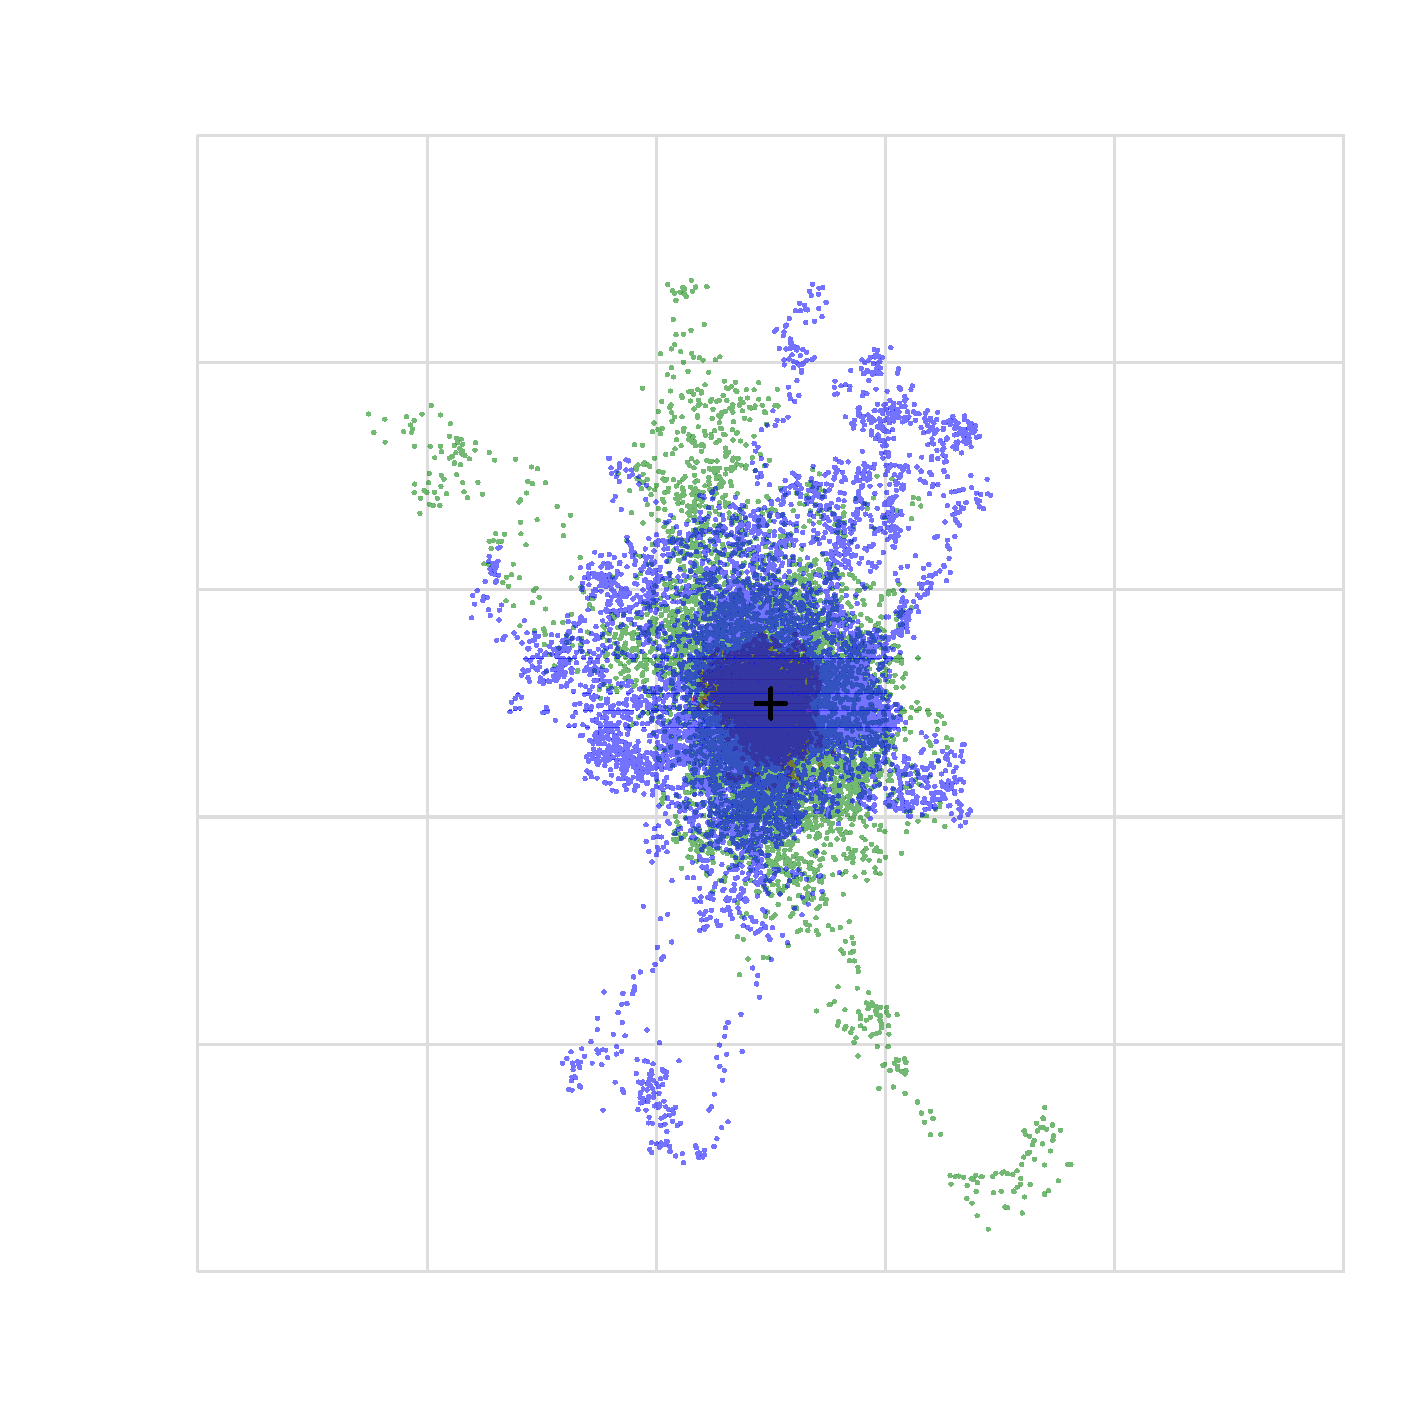
\includegraphics[width=680.0bp,height=680.0bp]{bericht/abbildungen/horizontal_zh.pdf}}
\put(95.0,657.0){\makebox(0,0)[lb]{\color{black}\sffamily\fontsize{16}{16}\selectfont {\cjkfont 相}\allowbreak{}{\cjkfont 对}\allowbreak{}{\cjkfont 于}\allowbreak{}{\cjkfont 同}\allowbreak{}{\cjkfont 一}\allowbreak{}{\cjkfont 时}\allowbreak{}{\cjkfont 刻}\allowbreak{}{\cjkfont 理}\allowbreak{}{\cjkfont 论}\allowbreak{}{\cjkfont 圆}\allowbreak{}{\cjkfont 周}\allowbreak{}{\cjkfont 位}\allowbreak{}{\cjkfont 置}\allowbreak{}{\cjkfont 的}\allowbreak{}{\cjkfont 水}\allowbreak{}{\cjkfont 平}\allowbreak{}{\cjkfont 误}\allowbreak{}{\cjkfont 差}\allowbreak{}}}
\put(95.0,50.0){\makebox(0,0)[cb]{\color{black}\sffamily\fontsize{12}{12}\selectfont -0.09642}}
\put(87.0,66.0){\makebox(0,0)[rb]{\color{black}\sffamily\fontsize{12}{12}\selectfont -0.09642}}
\put(205.0,50.0){\makebox(0,0)[cb]{\color{black}\sffamily\fontsize{12}{12}\selectfont -0.05785}}
\put(87.0,175.0){\makebox(0,0)[rb]{\color{black}\sffamily\fontsize{12}{12}\selectfont -0.05785}}
\put(315.0,50.0){\makebox(0,0)[cb]{\color{black}\sffamily\fontsize{12}{12}\selectfont -0.01928}}
\put(87.0,284.0){\makebox(0,0)[rb]{\color{black}\sffamily\fontsize{12}{12}\selectfont -0.01928}}
\put(425.00000000000006,50.0){\makebox(0,0)[cb]{\color{black}\sffamily\fontsize{12}{12}\selectfont 0.01928}}
\put(87.0,393.00000000000006){\makebox(0,0)[rb]{\color{black}\sffamily\fontsize{12}{12}\selectfont 0.01928}}
\put(535.0,50.0){\makebox(0,0)[cb]{\color{black}\sffamily\fontsize{12}{12}\selectfont 0.05785}}
\put(87.0,501.99999999999994){\makebox(0,0)[rb]{\color{black}\sffamily\fontsize{12}{12}\selectfont 0.05785}}
\put(645.0,50.0){\makebox(0,0)[cb]{\color{black}\sffamily\fontsize{12}{12}\selectfont 0.09642}}
\put(87.0,611.0){\makebox(0,0)[rb]{\color{black}\sffamily\fontsize{12}{12}\selectfont 0.09642}}
\put(95.0,635.0){\makebox(0,0)[lb]{\color{red}\sffamily\fontsize{12}{12}\selectfont P23A\_0}}
\put(265.0,635.0){\makebox(0,0)[lb]{\color{green}\sffamily\fontsize{12}{12}\selectfont P23A\_1}}
\put(435.0,635.0){\makebox(0,0)[lb]{\color{blue}\sffamily\fontsize{12}{12}\selectfont UM980}}
\put(379.0,351.5){\makebox(0,0)[lb]{\color{black}\sffamily\fontsize{12}{12}\selectfont {\cjkfont 理}\allowbreak{}{\cjkfont 论}\allowbreak{}{\cjkfont 值}\allowbreak{} (0,0)}}
\put(370.0,12.0){\makebox(0,0)[cb]{\color{black}\sffamily\fontsize{12}{12}\selectfont {\cjkfont 东}\allowbreak{}{\cjkfont 向}\allowbreak{}{\cjkfont 误}\allowbreak{}{\cjkfont 差}\allowbreak{} [m]}}
\put(19.0,342.5){\rotatebox{90}{\makebox(0,0)[b]{\color{black}\sffamily\fontsize{12}{12}\selectfont {\cjkfont 北}\allowbreak{}{\cjkfont 向}\allowbreak{}{\cjkfont 误}\allowbreak{}{\cjkfont 差}\allowbreak{} [m]}}}
\end{picture}}
\end{figure}
\begin{figure}[p]\centering
\resizebox{0.98\linewidth}{!}{%
\setlength{\unitlength}{1bp}\begin{picture}(680.0,680.0)
\put(0,0){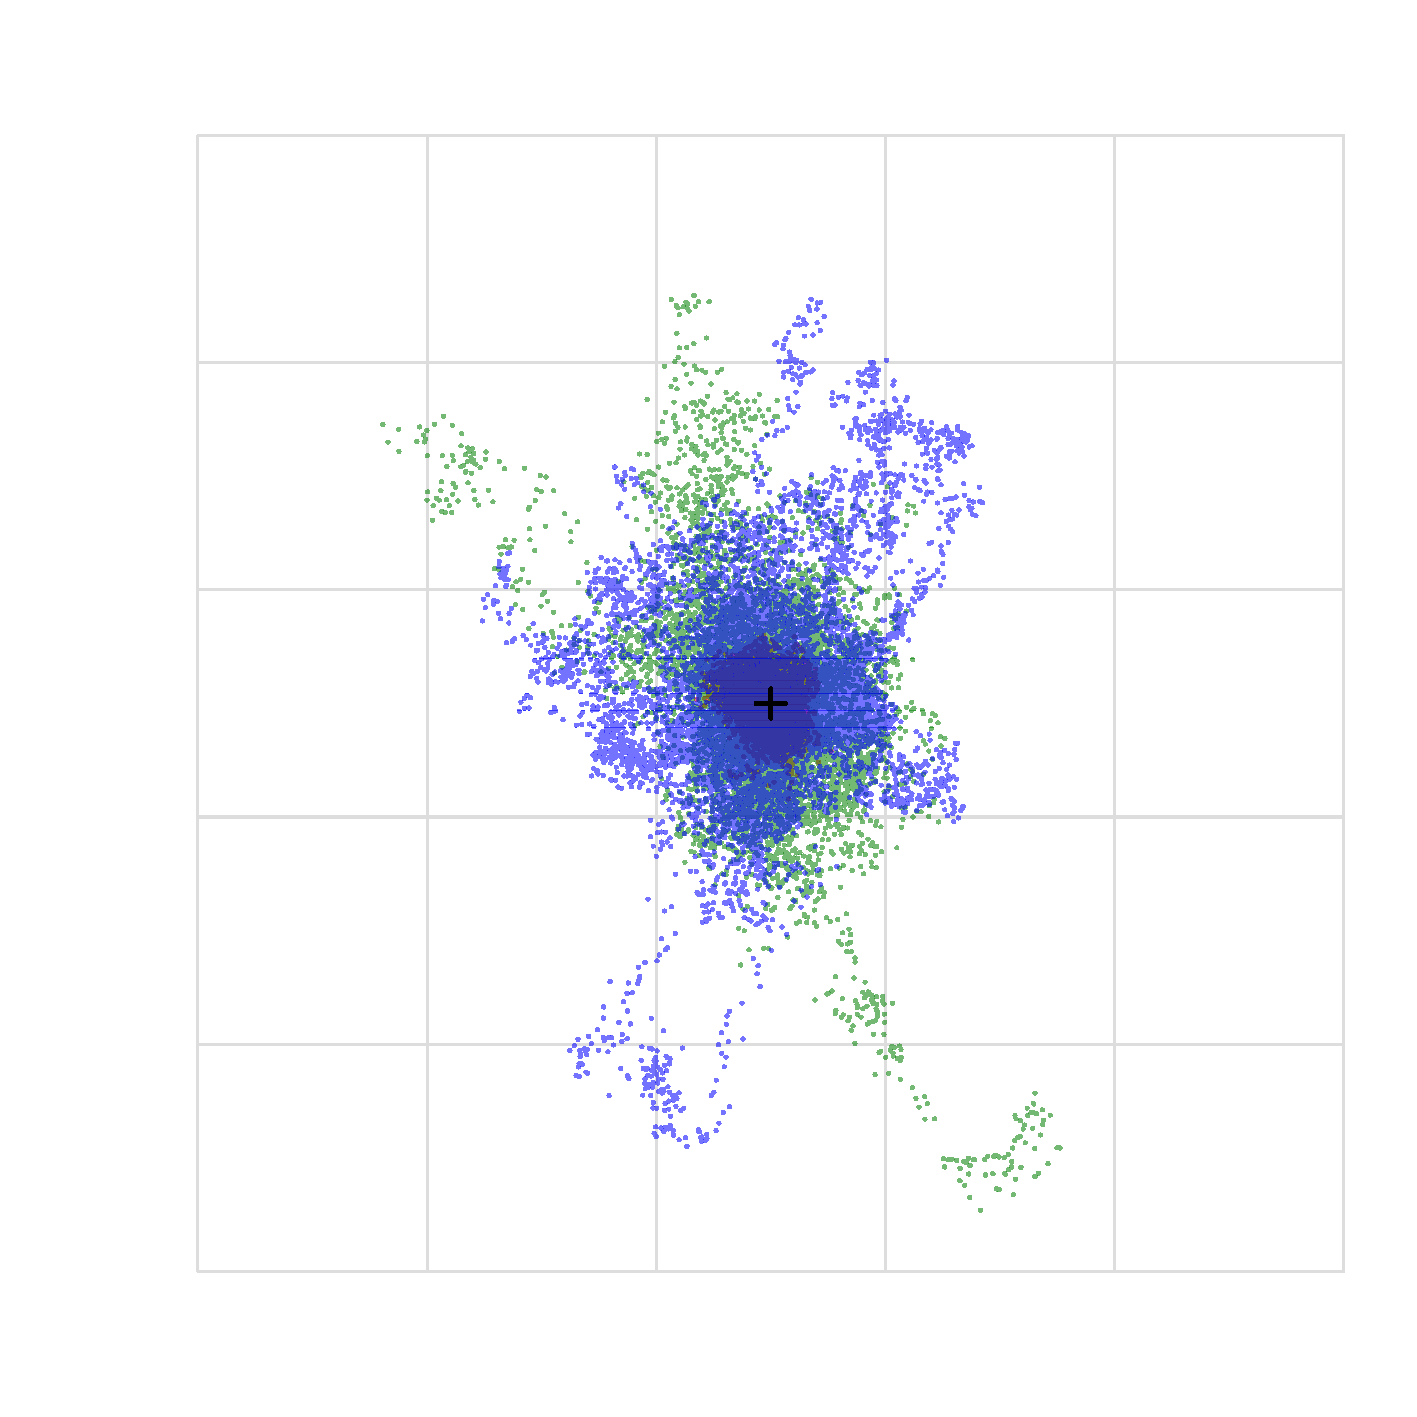
\includegraphics[width=680.0bp,height=680.0bp]{bericht/abbildungen/horizontal_detail_zh.pdf}}
\put(95.0,657.0){\makebox(0,0)[lb]{\color{black}\sffamily\fontsize{16}{16}\selectfont {\cjkfont 局}\allowbreak{}{\cjkfont 部}\allowbreak{}{\cjkfont 视}\allowbreak{}{\cjkfont 图}\allowbreak{} ±0.10 m{\cjkfont （}\allowbreak{}{\cjkfont 不}\allowbreak{}{\cjkfont 显}\allowbreak{}{\cjkfont 示}\allowbreak{}{\cjkfont 范}\allowbreak{}{\cjkfont 围}\allowbreak{}{\cjkfont 外}\allowbreak{}{\cjkfont 的}\allowbreak{}{\cjkfont 误}\allowbreak{}{\cjkfont 差}\allowbreak{}{\cjkfont ）}\allowbreak{}}}
\put(95.0,50.0){\makebox(0,0)[cb]{\color{black}\sffamily\fontsize{12}{12}\selectfont -0.1}}
\put(87.0,66.0){\makebox(0,0)[rb]{\color{black}\sffamily\fontsize{12}{12}\selectfont -0.1}}
\put(205.0,50.0){\makebox(0,0)[cb]{\color{black}\sffamily\fontsize{12}{12}\selectfont -0.06}}
\put(87.0,175.0){\makebox(0,0)[rb]{\color{black}\sffamily\fontsize{12}{12}\selectfont -0.06}}
\put(315.0,50.0){\makebox(0,0)[cb]{\color{black}\sffamily\fontsize{12}{12}\selectfont -0.02}}
\put(87.0,284.0){\makebox(0,0)[rb]{\color{black}\sffamily\fontsize{12}{12}\selectfont -0.02}}
\put(425.00000000000006,50.0){\makebox(0,0)[cb]{\color{black}\sffamily\fontsize{12}{12}\selectfont 0.02}}
\put(87.0,393.00000000000006){\makebox(0,0)[rb]{\color{black}\sffamily\fontsize{12}{12}\selectfont 0.02}}
\put(535.0,50.0){\makebox(0,0)[cb]{\color{black}\sffamily\fontsize{12}{12}\selectfont 0.06}}
\put(87.0,501.99999999999994){\makebox(0,0)[rb]{\color{black}\sffamily\fontsize{12}{12}\selectfont 0.06}}
\put(645.0,50.0){\makebox(0,0)[cb]{\color{black}\sffamily\fontsize{12}{12}\selectfont 0.1}}
\put(87.0,611.0){\makebox(0,0)[rb]{\color{black}\sffamily\fontsize{12}{12}\selectfont 0.1}}
\put(95.0,635.0){\makebox(0,0)[lb]{\color{red}\sffamily\fontsize{12}{12}\selectfont P23A\_0}}
\put(265.0,635.0){\makebox(0,0)[lb]{\color{green}\sffamily\fontsize{12}{12}\selectfont P23A\_1}}
\put(435.0,635.0){\makebox(0,0)[lb]{\color{blue}\sffamily\fontsize{12}{12}\selectfont UM980}}
\put(379.0,351.5){\makebox(0,0)[lb]{\color{black}\sffamily\fontsize{12}{12}\selectfont {\cjkfont 理}\allowbreak{}{\cjkfont 论}\allowbreak{}{\cjkfont 值}\allowbreak{} (0,0)}}
\put(370.0,12.0){\makebox(0,0)[cb]{\color{black}\sffamily\fontsize{12}{12}\selectfont {\cjkfont 东}\allowbreak{}{\cjkfont 向}\allowbreak{}{\cjkfont 误}\allowbreak{}{\cjkfont 差}\allowbreak{} [m]}}
\put(19.0,342.5){\rotatebox{90}{\makebox(0,0)[b]{\color{black}\sffamily\fontsize{12}{12}\selectfont {\cjkfont 北}\allowbreak{}{\cjkfont 向}\allowbreak{}{\cjkfont 误}\allowbreak{}{\cjkfont 差}\allowbreak{} [m]}}}
\end{picture}}
\end{figure}
\begin{figure}[p]\centering
\resizebox{0.98\linewidth}{!}{%
\setlength{\unitlength}{1bp}\begin{picture}(1000.0,430.0)
\put(0,0){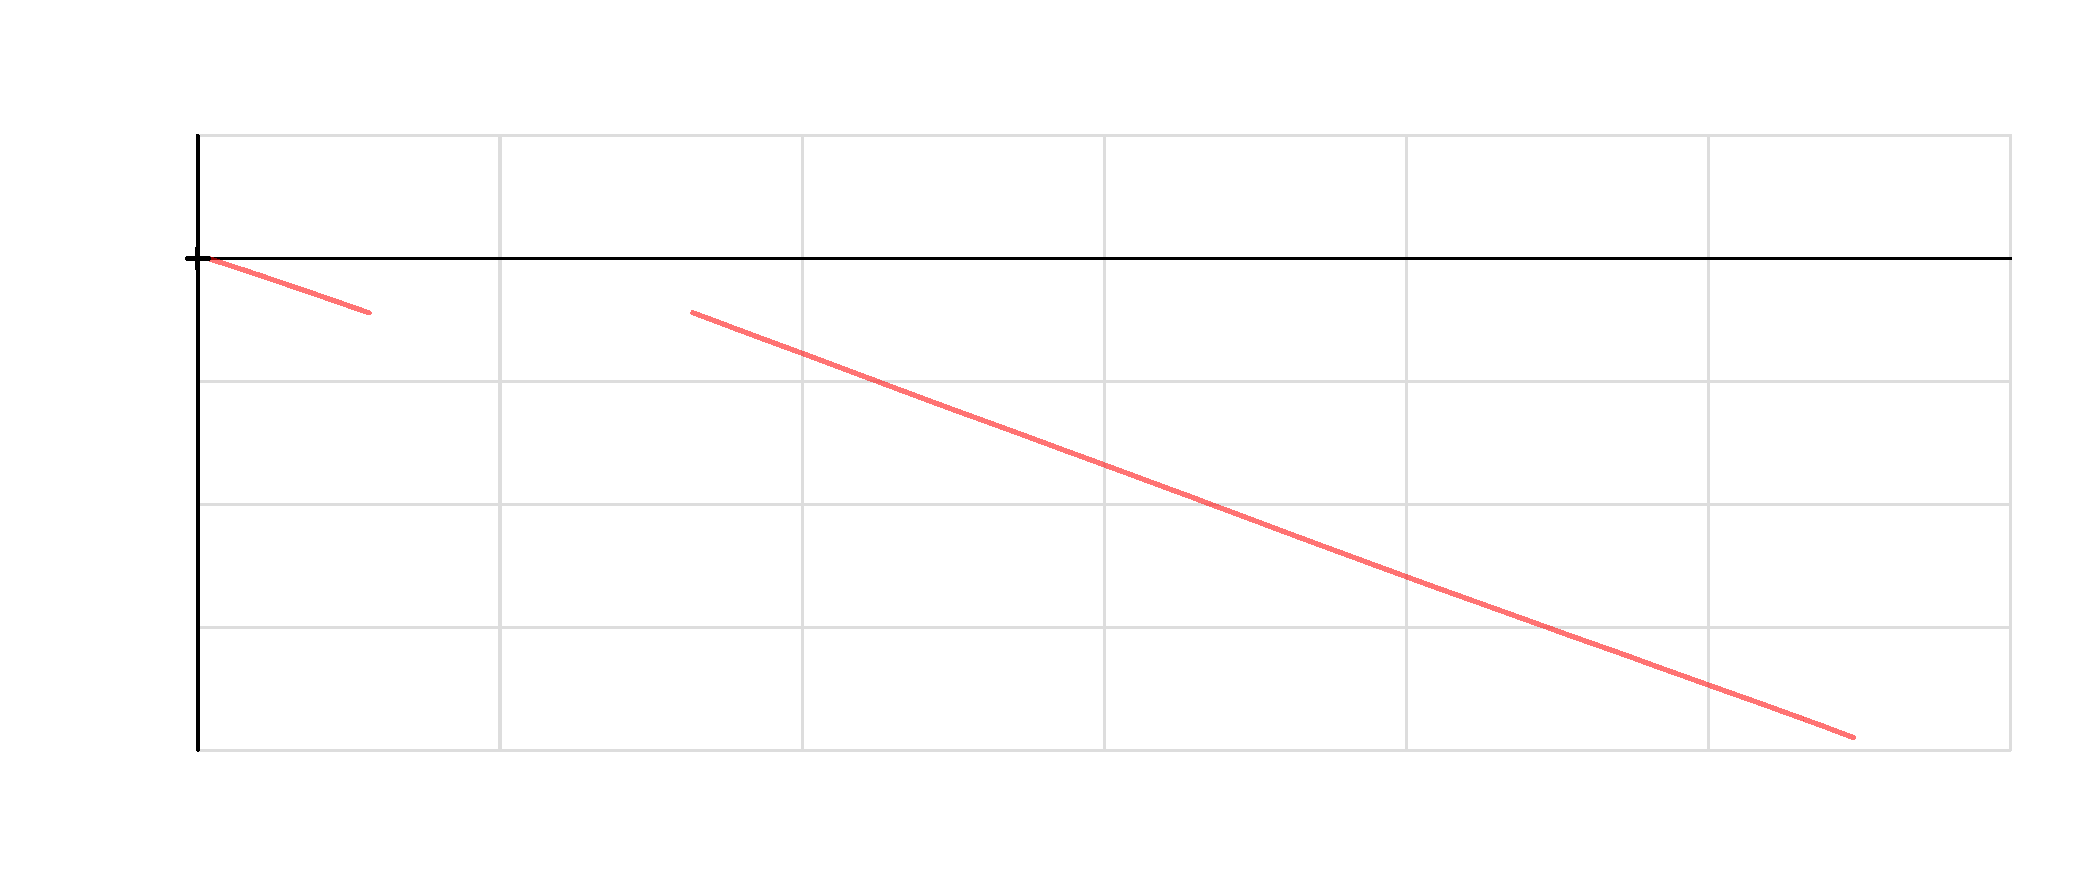
\includegraphics[width=1000.0bp,height=430.0bp]{bericht/abbildungen/winkel_zh.pdf}}
\put(95.0,407.0){\makebox(0,0)[lb]{\color{black}\sffamily\fontsize{16}{16}\selectfont {\cjkfont 旋}\allowbreak{}{\cjkfont 转}\allowbreak{}{\cjkfont 圈}\allowbreak{}{\cjkfont 数}\allowbreak{}{\cjkfont ：}\allowbreak{}{\cjkfont 从}\allowbreak{}{\cjkfont 东}\allowbreak{}{\cjkfont 向}\allowbreak{}{\cjkfont 北}\allowbreak{}{\cjkfont 为}\allowbreak{}{\cjkfont 正}\allowbreak{}{\cjkfont 方}\allowbreak{}{\cjkfont 向}\allowbreak{}}}
\put(95.0,50.0){\makebox(0,0)[cb]{\color{black}\sffamily\fontsize{12}{12}\selectfont -10.96}}
\put(87.0,66.0){\makebox(0,0)[rb]{\color{black}\sffamily\fontsize{12}{12}\selectfont -84.19}}
\put(269.0,50.0){\makebox(0,0)[cb]{\color{black}\sffamily\fontsize{12}{12}\selectfont 48.22}}
\put(87.0,125.0){\makebox(0,0)[rb]{\color{black}\sffamily\fontsize{12}{12}\selectfont -66.1}}
\put(442.99999999999994,50.0){\makebox(0,0)[cb]{\color{black}\sffamily\fontsize{12}{12}\selectfont 107.4}}
\put(87.0,184.0){\makebox(0,0)[rb]{\color{black}\sffamily\fontsize{12}{12}\selectfont -48.02}}
\put(617.0000000000001,50.0){\makebox(0,0)[cb]{\color{black}\sffamily\fontsize{12}{12}\selectfont 166.6}}
\put(87.0,243.00000000000003){\makebox(0,0)[rb]{\color{black}\sffamily\fontsize{12}{12}\selectfont -29.93}}
\put(790.9999999999999,50.0){\makebox(0,0)[cb]{\color{black}\sffamily\fontsize{12}{12}\selectfont 225.8}}
\put(87.0,302.0){\makebox(0,0)[rb]{\color{black}\sffamily\fontsize{12}{12}\selectfont -11.85}}
\put(965.0,50.0){\makebox(0,0)[cb]{\color{black}\sffamily\fontsize{12}{12}\selectfont 284.9}}
\put(87.0,361.0){\makebox(0,0)[rb]{\color{black}\sffamily\fontsize{12}{12}\selectfont 6.24}}
\put(95.0,385.0){\makebox(0,0)[lb]{\color{red}\sffamily\fontsize{12}{12}\selectfont P23A\_0}}
\put(530.0,12.0){\makebox(0,0)[cb]{\color{black}\sffamily\fontsize{12}{12}\selectfont {\cjkfont 自}\allowbreak{}{\cjkfont 共}\allowbreak{}{\cjkfont 同}\allowbreak{}{\cjkfont 起}\allowbreak{}{\cjkfont 始}\allowbreak{}{\cjkfont 时}\allowbreak{}{\cjkfont 刻}\allowbreak{}{\cjkfont 起}\allowbreak{}{\cjkfont 的}\allowbreak{}{\cjkfont 时}\allowbreak{}{\cjkfont 间}\allowbreak{} [min]}}
\put(19.0,217.5){\rotatebox{90}{\makebox(0,0)[b]{\color{black}\sffamily\fontsize{12}{12}\selectfont {\cjkfont 自}\allowbreak{}{\cjkfont 首}\allowbreak{}{\cjkfont 个}\allowbreak{}{\cjkfont 参}\allowbreak{}{\cjkfont 考}\allowbreak{}{\cjkfont 点}\allowbreak{}{\cjkfont 起}\allowbreak{}{\cjkfont 的}\allowbreak{}{\cjkfont 旋}\allowbreak{}{\cjkfont 转}\allowbreak{}{\cjkfont 圈}\allowbreak{}{\cjkfont 数}\allowbreak{}}}}
\end{picture}}
\end{figure}
\begin{figure}[p]\centering
\resizebox{0.98\linewidth}{!}{%
\setlength{\unitlength}{1bp}\begin{picture}(1000.0,430.0)
\put(0,0){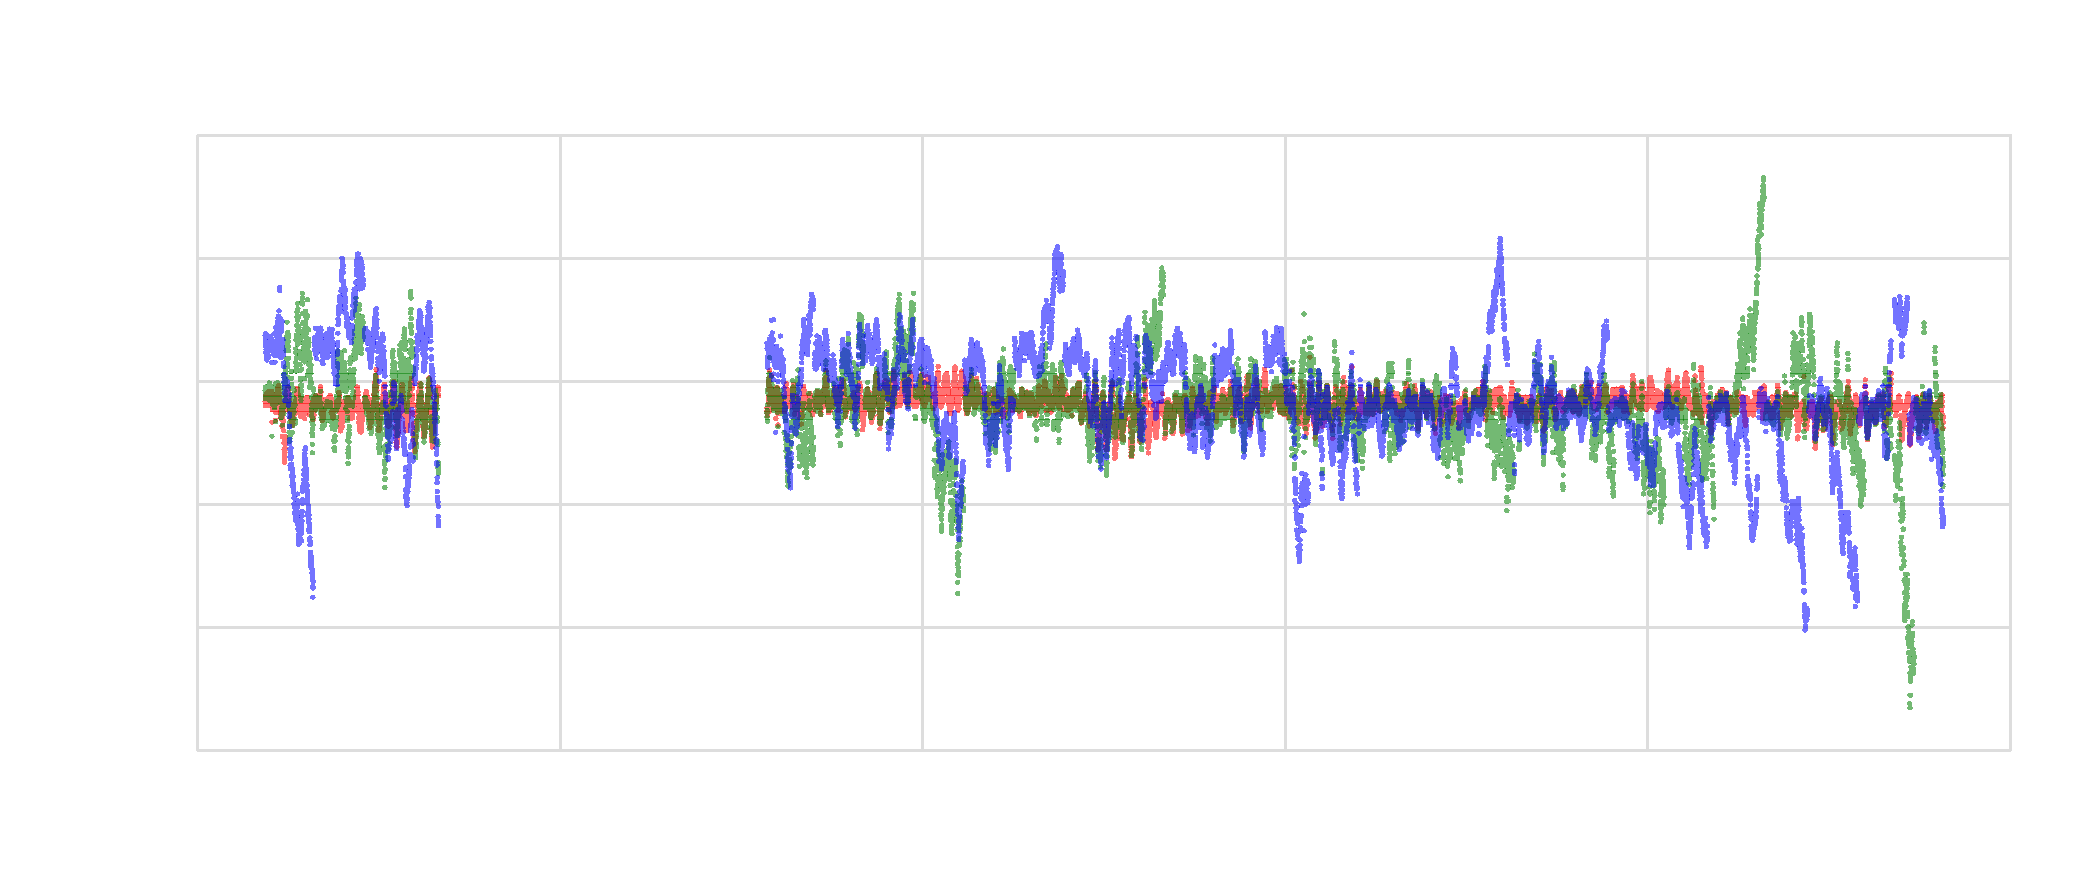
\includegraphics[width=1000.0bp,height=430.0bp]{bericht/abbildungen/east_zeit_zh.pdf}}
\put(95.0,407.0){\makebox(0,0)[lb]{\color{black}\sffamily\fontsize{16}{16}\selectfont {\cjkfont 东}\allowbreak{}{\cjkfont 向}\allowbreak{}{\cjkfont 误}\allowbreak{}{\cjkfont 差}\allowbreak{}{\cjkfont 随}\allowbreak{}{\cjkfont 时}\allowbreak{}{\cjkfont 间}\allowbreak{}{\cjkfont 的}\allowbreak{}{\cjkfont 变}\allowbreak{}{\cjkfont 化}\allowbreak{}}}
\put(95.0,50.0){\makebox(0,0)[cb]{\color{black}\sffamily\fontsize{12}{12}\selectfont -10.96}}
\put(87.0,66.0){\makebox(0,0)[rb]{\color{black}\sffamily\fontsize{12}{12}\selectfont -0.0772}}
\put(269.0,50.0){\makebox(0,0)[cb]{\color{black}\sffamily\fontsize{12}{12}\selectfont 48.22}}
\put(87.0,125.0){\makebox(0,0)[rb]{\color{black}\sffamily\fontsize{12}{12}\selectfont -0.04977}}
\put(442.99999999999994,50.0){\makebox(0,0)[cb]{\color{black}\sffamily\fontsize{12}{12}\selectfont 107.4}}
\put(87.0,184.0){\makebox(0,0)[rb]{\color{black}\sffamily\fontsize{12}{12}\selectfont -0.02235}}
\put(617.0000000000001,50.0){\makebox(0,0)[cb]{\color{black}\sffamily\fontsize{12}{12}\selectfont 166.6}}
\put(87.0,243.0){\makebox(0,0)[rb]{\color{black}\sffamily\fontsize{12}{12}\selectfont 0.005077}}
\put(790.9999999999999,50.0){\makebox(0,0)[cb]{\color{black}\sffamily\fontsize{12}{12}\selectfont 225.8}}
\put(87.0,302.0){\makebox(0,0)[rb]{\color{black}\sffamily\fontsize{12}{12}\selectfont 0.0325}}
\put(965.0,50.0){\makebox(0,0)[cb]{\color{black}\sffamily\fontsize{12}{12}\selectfont 284.9}}
\put(87.0,361.0){\makebox(0,0)[rb]{\color{black}\sffamily\fontsize{12}{12}\selectfont 0.05993}}
\put(95.0,385.0){\makebox(0,0)[lb]{\color{red}\sffamily\fontsize{12}{12}\selectfont P23A\_0}}
\put(265.0,385.0){\makebox(0,0)[lb]{\color{green}\sffamily\fontsize{12}{12}\selectfont P23A\_1}}
\put(435.0,385.0){\makebox(0,0)[lb]{\color{blue}\sffamily\fontsize{12}{12}\selectfont UM980}}
\put(530.0,12.0){\makebox(0,0)[cb]{\color{black}\sffamily\fontsize{12}{12}\selectfont {\cjkfont 自}\allowbreak{}{\cjkfont 共}\allowbreak{}{\cjkfont 同}\allowbreak{}{\cjkfont 起}\allowbreak{}{\cjkfont 始}\allowbreak{}{\cjkfont 时}\allowbreak{}{\cjkfont 刻}\allowbreak{}{\cjkfont 起}\allowbreak{}{\cjkfont 的}\allowbreak{}{\cjkfont 时}\allowbreak{}{\cjkfont 间}\allowbreak{} [min]}}
\put(19.0,217.5){\rotatebox{90}{\makebox(0,0)[b]{\color{black}\sffamily\fontsize{12}{12}\selectfont {\cjkfont 东}\allowbreak{}{\cjkfont 向}\allowbreak{}{\cjkfont 误}\allowbreak{}{\cjkfont 差}\allowbreak{} [m]}}}
\end{picture}}
\end{figure}
\begin{figure}[p]\centering
\resizebox{0.98\linewidth}{!}{%
\setlength{\unitlength}{1bp}\begin{picture}(1000.0,430.0)
\put(0,0){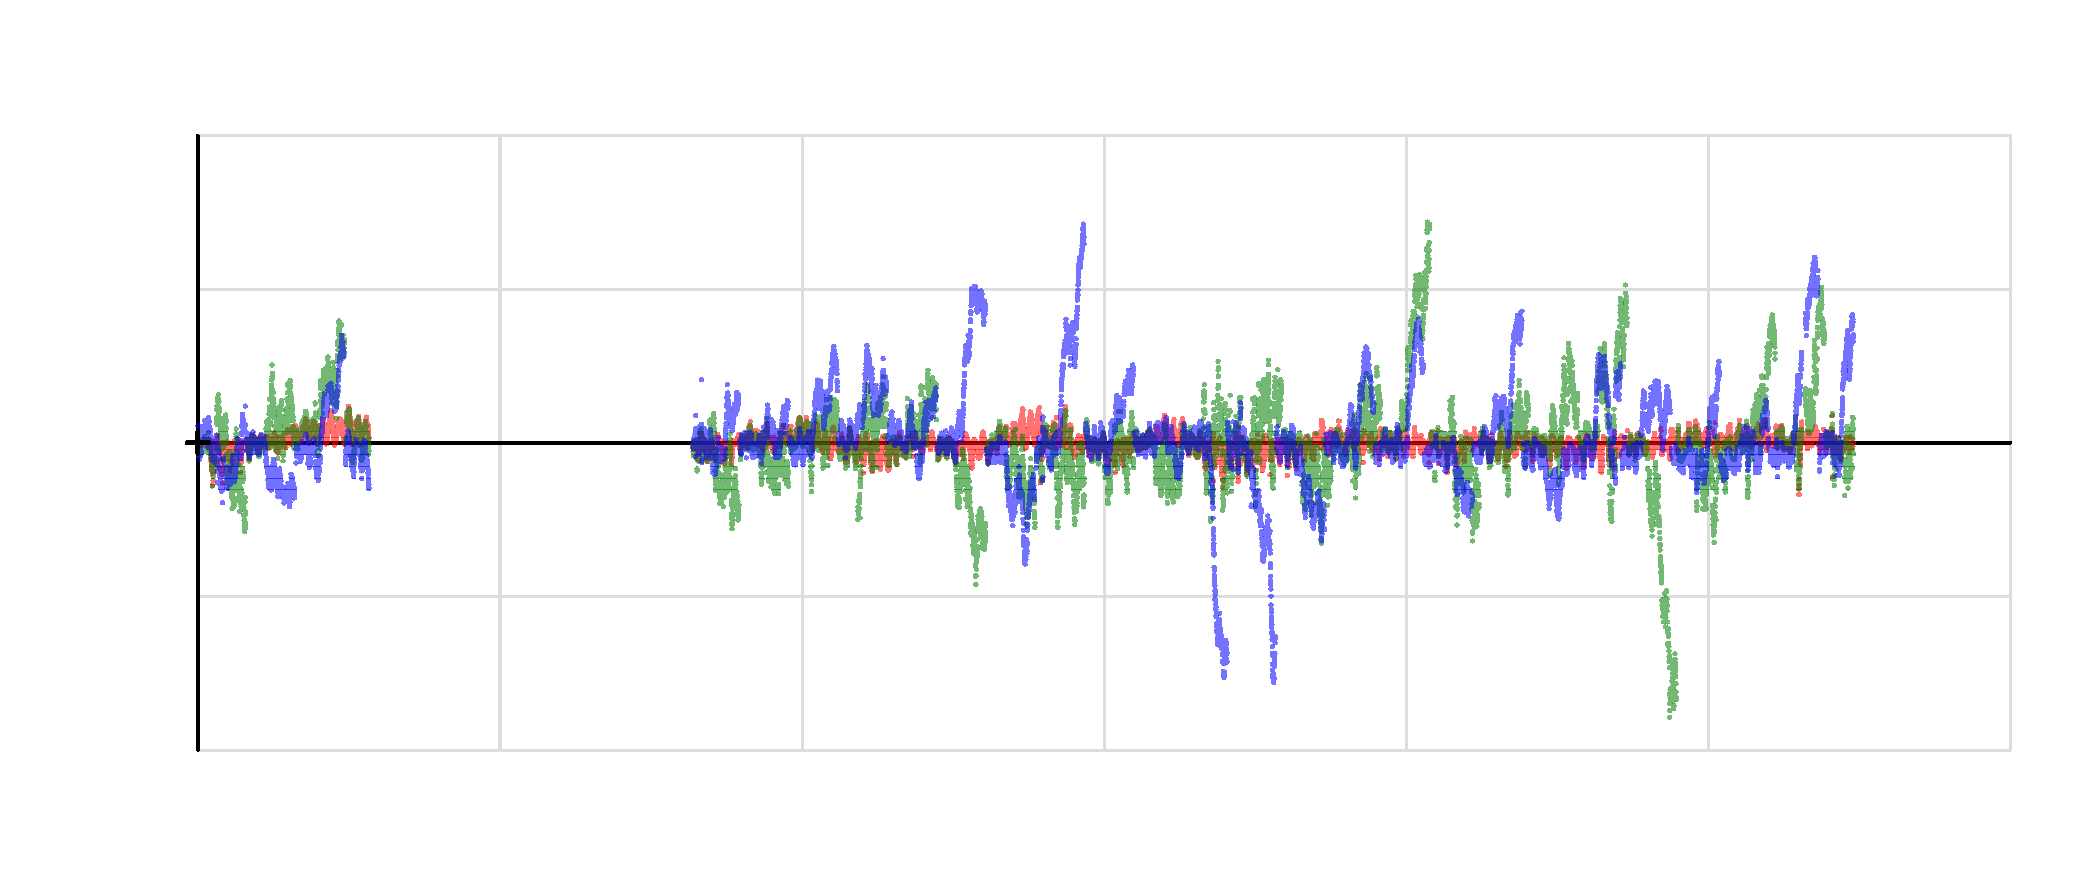
\includegraphics[width=1000.0bp,height=430.0bp]{bericht/abbildungen/north_zeit_zh.pdf}}
\put(95.0,407.0){\makebox(0,0)[lb]{\color{black}\sffamily\fontsize{16}{16}\selectfont {\cjkfont 北}\allowbreak{}{\cjkfont 向}\allowbreak{}{\cjkfont 误}\allowbreak{}{\cjkfont 差}\allowbreak{}{\cjkfont 随}\allowbreak{}{\cjkfont 时}\allowbreak{}{\cjkfont 间}\allowbreak{}{\cjkfont 的}\allowbreak{}{\cjkfont 变}\allowbreak{}{\cjkfont 化}\allowbreak{}}}
\put(95.0,50.0){\makebox(0,0)[cb]{\color{black}\sffamily\fontsize{12}{12}\selectfont -10.96}}
\put(87.0,66.0){\makebox(0,0)[rb]{\color{black}\sffamily\fontsize{12}{12}\selectfont -0.1022}}
\put(269.0,50.0){\makebox(0,0)[cb]{\color{black}\sffamily\fontsize{12}{12}\selectfont 48.22}}
\put(87.0,125.0){\makebox(0,0)[rb]{\color{black}\sffamily\fontsize{12}{12}\selectfont -0.06478}}
\put(442.99999999999994,50.0){\makebox(0,0)[cb]{\color{black}\sffamily\fontsize{12}{12}\selectfont 107.4}}
\put(87.0,184.0){\makebox(0,0)[rb]{\color{black}\sffamily\fontsize{12}{12}\selectfont -0.0274}}
\put(617.0000000000001,50.0){\makebox(0,0)[cb]{\color{black}\sffamily\fontsize{12}{12}\selectfont 166.6}}
\put(87.0,243.0){\makebox(0,0)[rb]{\color{black}\sffamily\fontsize{12}{12}\selectfont 0.00999}}
\put(790.9999999999999,50.0){\makebox(0,0)[cb]{\color{black}\sffamily\fontsize{12}{12}\selectfont 225.8}}
\put(87.0,302.0){\makebox(0,0)[rb]{\color{black}\sffamily\fontsize{12}{12}\selectfont 0.04738}}
\put(965.0,50.0){\makebox(0,0)[cb]{\color{black}\sffamily\fontsize{12}{12}\selectfont 284.9}}
\put(87.0,361.0){\makebox(0,0)[rb]{\color{black}\sffamily\fontsize{12}{12}\selectfont 0.08476}}
\put(95.0,385.0){\makebox(0,0)[lb]{\color{red}\sffamily\fontsize{12}{12}\selectfont P23A\_0}}
\put(265.0,385.0){\makebox(0,0)[lb]{\color{green}\sffamily\fontsize{12}{12}\selectfont P23A\_1}}
\put(435.0,385.0){\makebox(0,0)[lb]{\color{blue}\sffamily\fontsize{12}{12}\selectfont UM980}}
\put(530.0,12.0){\makebox(0,0)[cb]{\color{black}\sffamily\fontsize{12}{12}\selectfont {\cjkfont 自}\allowbreak{}{\cjkfont 共}\allowbreak{}{\cjkfont 同}\allowbreak{}{\cjkfont 起}\allowbreak{}{\cjkfont 始}\allowbreak{}{\cjkfont 时}\allowbreak{}{\cjkfont 刻}\allowbreak{}{\cjkfont 起}\allowbreak{}{\cjkfont 的}\allowbreak{}{\cjkfont 时}\allowbreak{}{\cjkfont 间}\allowbreak{} [min]}}
\put(19.0,217.5){\rotatebox{90}{\makebox(0,0)[b]{\color{black}\sffamily\fontsize{12}{12}\selectfont {\cjkfont 北}\allowbreak{}{\cjkfont 向}\allowbreak{}{\cjkfont 误}\allowbreak{}{\cjkfont 差}\allowbreak{} [m]}}}
\end{picture}}
\end{figure}
\begin{figure}[p]\centering
\resizebox{0.98\linewidth}{!}{%
\setlength{\unitlength}{1bp}\begin{picture}(1000.0,430.0)
\put(0,0){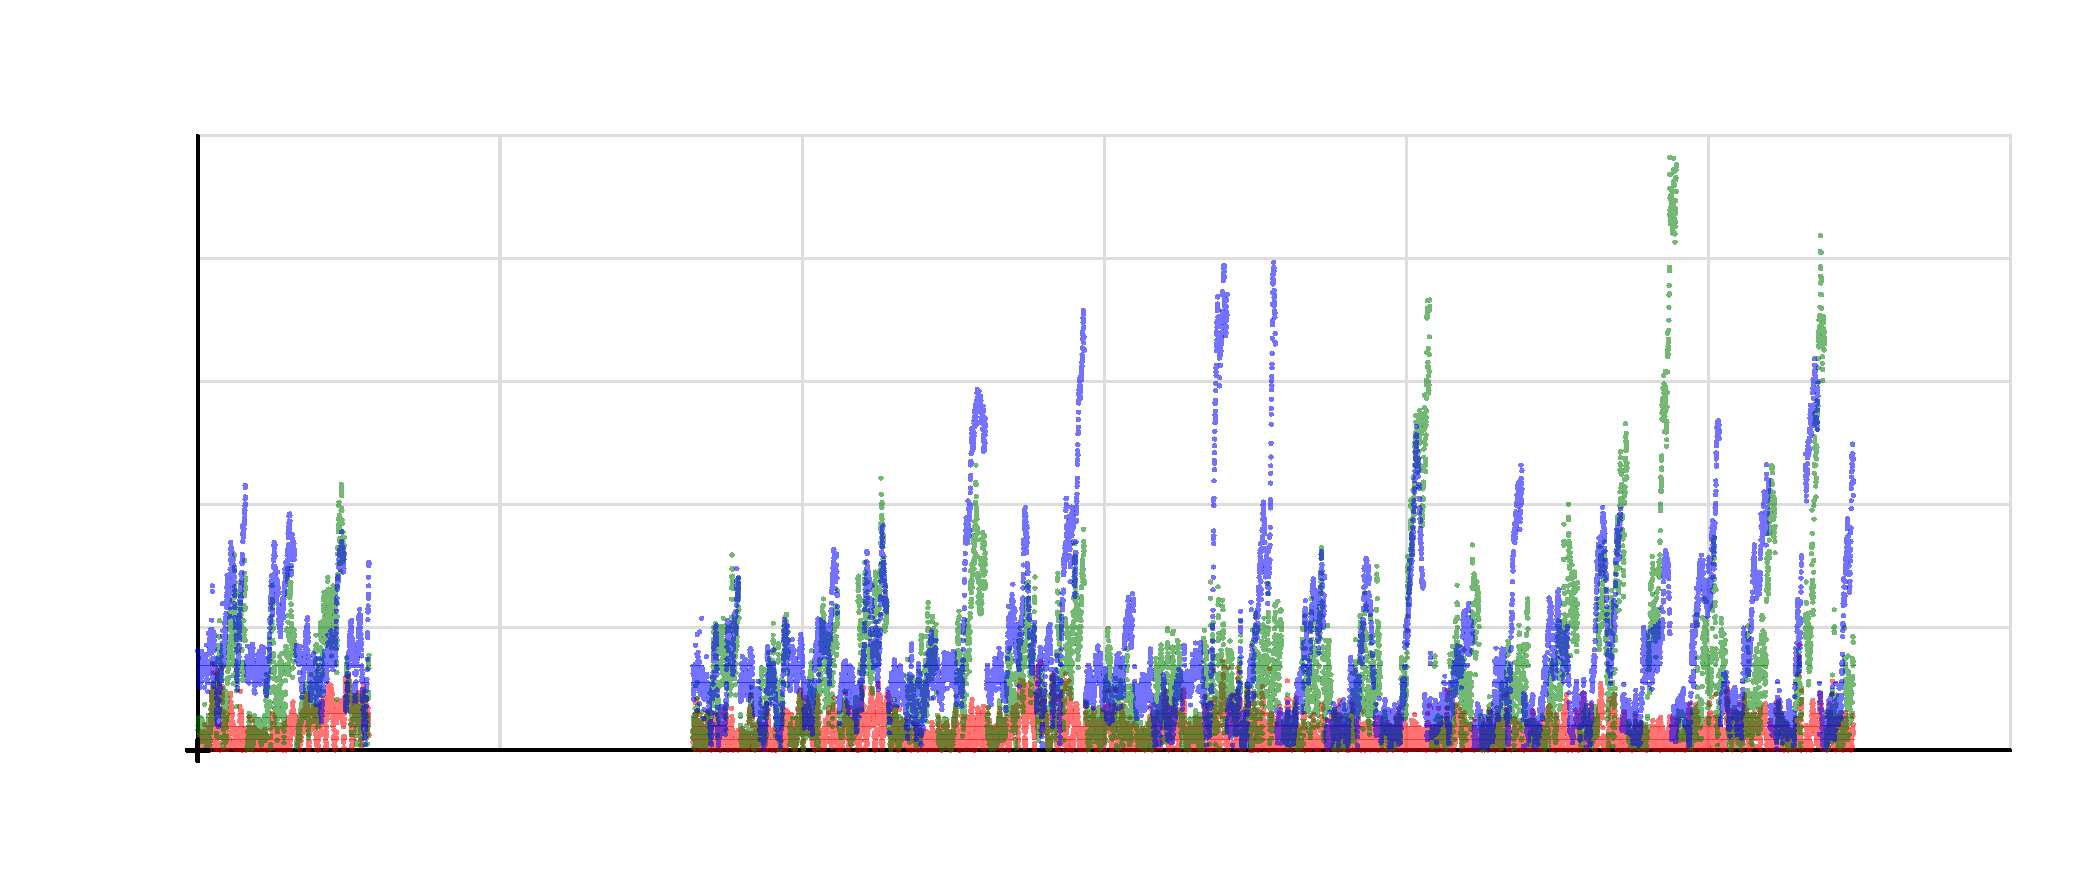
\includegraphics[width=1000.0bp,height=430.0bp]{bericht/abbildungen/horizontal_zeit_zh.pdf}}
\put(95.0,407.0){\makebox(0,0)[lb]{\color{black}\sffamily\fontsize{16}{16}\selectfont {\cjkfont 水}\allowbreak{}{\cjkfont 平}\allowbreak{}{\cjkfont 误}\allowbreak{}{\cjkfont 差}\allowbreak{}{\cjkfont 随}\allowbreak{}{\cjkfont 时}\allowbreak{}{\cjkfont 间}\allowbreak{}{\cjkfont 的}\allowbreak{}{\cjkfont 变}\allowbreak{}{\cjkfont 化}\allowbreak{}}}
\put(95.0,50.0){\makebox(0,0)[cb]{\color{black}\sffamily\fontsize{12}{12}\selectfont -10.96}}
\put(87.0,66.0){\makebox(0,0)[rb]{\color{black}\sffamily\fontsize{12}{12}\selectfont -0.007717}}
\put(269.0,50.0){\makebox(0,0)[cb]{\color{black}\sffamily\fontsize{12}{12}\selectfont 48.22}}
\put(87.0,125.0){\makebox(0,0)[rb]{\color{black}\sffamily\fontsize{12}{12}\selectfont 0.01466}}
\put(442.99999999999994,50.0){\makebox(0,0)[cb]{\color{black}\sffamily\fontsize{12}{12}\selectfont 107.4}}
\put(87.0,184.0){\makebox(0,0)[rb]{\color{black}\sffamily\fontsize{12}{12}\selectfont 0.03705}}
\put(617.0000000000001,50.0){\makebox(0,0)[cb]{\color{black}\sffamily\fontsize{12}{12}\selectfont 166.6}}
\put(87.0,243.0){\makebox(0,0)[rb]{\color{black}\sffamily\fontsize{12}{12}\selectfont 0.05943}}
\put(790.9999999999999,50.0){\makebox(0,0)[cb]{\color{black}\sffamily\fontsize{12}{12}\selectfont 225.8}}
\put(87.0,302.0){\makebox(0,0)[rb]{\color{black}\sffamily\fontsize{12}{12}\selectfont 0.08181}}
\put(965.0,50.0){\makebox(0,0)[cb]{\color{black}\sffamily\fontsize{12}{12}\selectfont 284.9}}
\put(87.0,361.0){\makebox(0,0)[rb]{\color{black}\sffamily\fontsize{12}{12}\selectfont 0.1042}}
\put(95.0,385.0){\makebox(0,0)[lb]{\color{red}\sffamily\fontsize{12}{12}\selectfont P23A\_0}}
\put(265.0,385.0){\makebox(0,0)[lb]{\color{green}\sffamily\fontsize{12}{12}\selectfont P23A\_1}}
\put(435.0,385.0){\makebox(0,0)[lb]{\color{blue}\sffamily\fontsize{12}{12}\selectfont UM980}}
\put(530.0,12.0){\makebox(0,0)[cb]{\color{black}\sffamily\fontsize{12}{12}\selectfont {\cjkfont 自}\allowbreak{}{\cjkfont 共}\allowbreak{}{\cjkfont 同}\allowbreak{}{\cjkfont 起}\allowbreak{}{\cjkfont 始}\allowbreak{}{\cjkfont 时}\allowbreak{}{\cjkfont 刻}\allowbreak{}{\cjkfont 起}\allowbreak{}{\cjkfont 的}\allowbreak{}{\cjkfont 时}\allowbreak{}{\cjkfont 间}\allowbreak{} [min]}}
\put(19.0,217.5){\rotatebox{90}{\makebox(0,0)[b]{\color{black}\sffamily\fontsize{12}{12}\selectfont {\cjkfont 水}\allowbreak{}{\cjkfont 平}\allowbreak{}{\cjkfont 误}\allowbreak{}{\cjkfont 差}\allowbreak{} [m]}}}
\end{picture}}
\end{figure}\clearpage
\end{document}
